\documentclass{article}
\usepackage{fontspec,tikz,graphicx}
\setmainfont{Times New Roman}
\usepackage[a3paper,margin=1cm]{geometry}
\pagestyle{empty}
\begin{document}
\noindent\resizebox{!}{0.96\textheight}{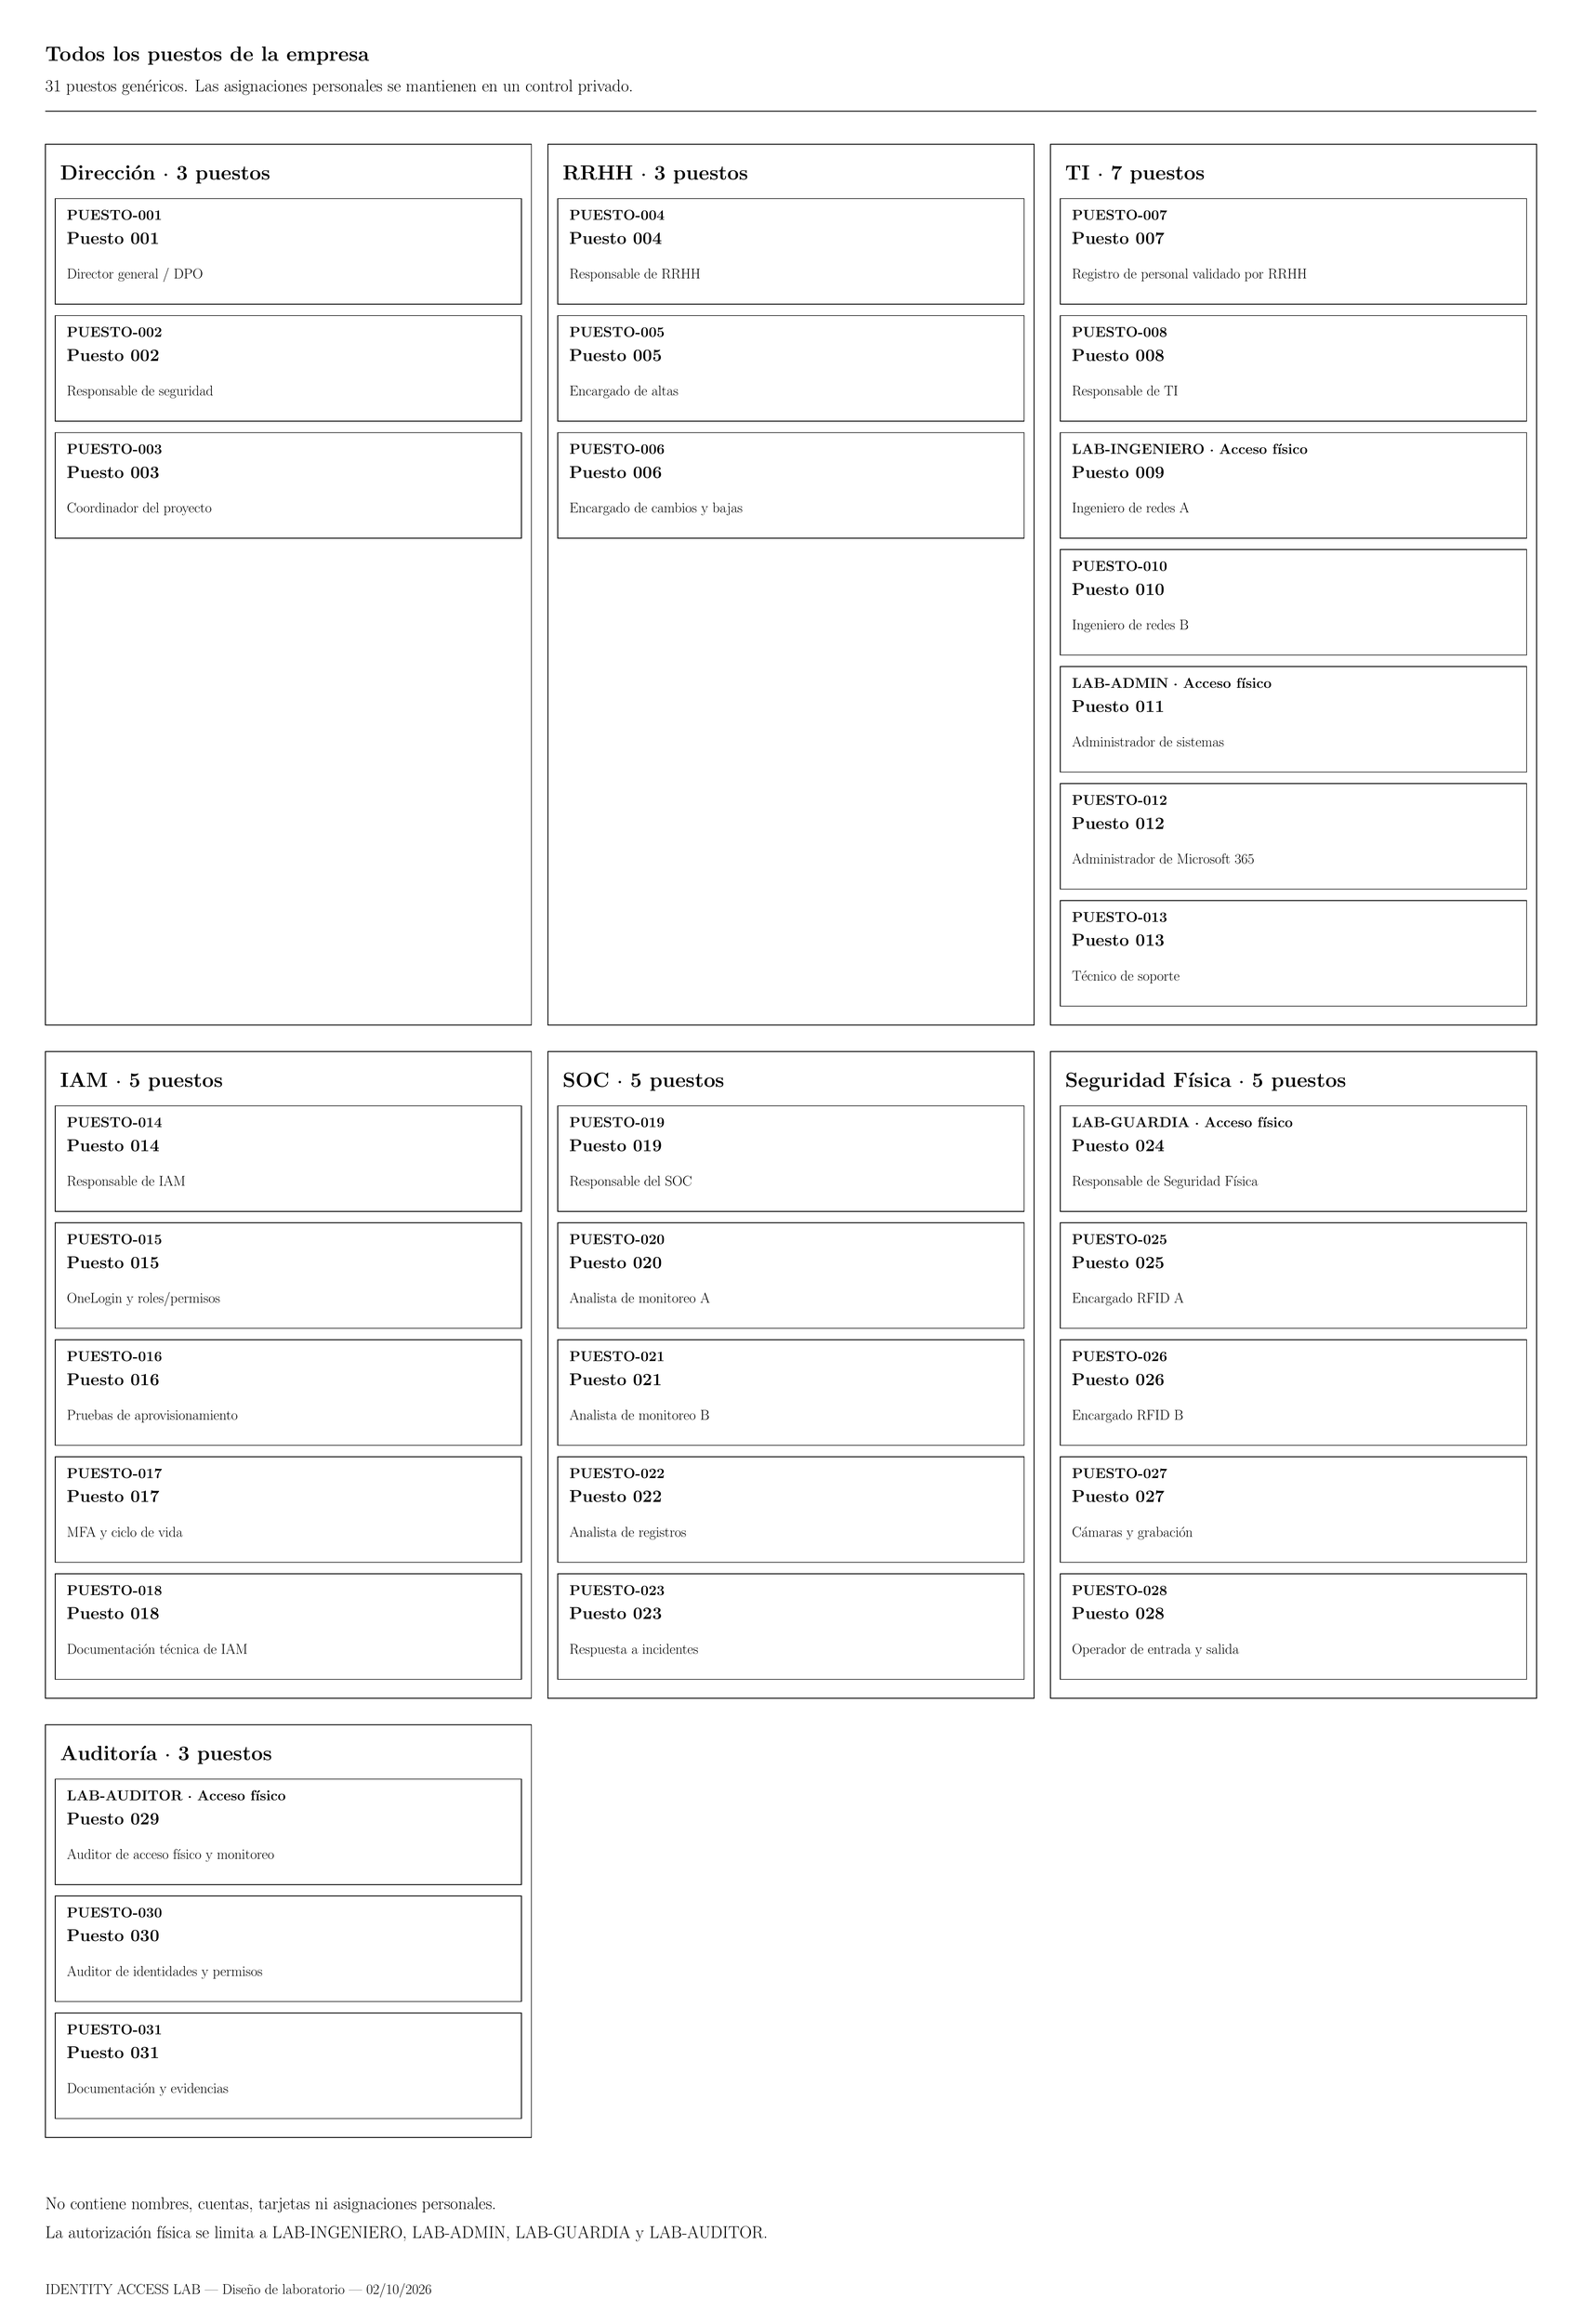
\begin{tikzpicture}[x=1pt,y=-1pt]
\path[use as bounding box] (0,0) rectangle (1900.0,2800.0);
\node[anchor=base west,inner sep=0pt,font=\fontsize{34.0}{40.8}\selectfont \bfseries ] at (45,64) {Todos los puestos de la empresa};
\node[anchor=base west,inner sep=0pt,font=\fontsize{21.0}{25.2}\selectfont ] at (45,101) {31 puestos genéricos. Las asignaciones personales se mantienen en un control privado.};
\draw[line width=1pt] (45,125) -- (1855,125);
\draw[line width=1pt] (45.0,165.0) rectangle (635.0,1234.0);
\node[anchor=base west,inner sep=0pt,font=\fontsize{25.0}{30.0}\selectfont \bfseries ] at (63,208) {Dirección · 3 puestos};
\draw[line width=1pt] (57.0,231.0) rectangle (623.0,359.0);
\node[anchor=base west,inner sep=0pt,font=\fontsize{18.0}{21.599999999999998}\selectfont \bfseries ] at (71,257) {PUESTO-001};
\node[anchor=base west,inner sep=0pt,font=\fontsize{20.0}{24.0}\selectfont \bfseries ] at (71,286) {Puesto 001};
\node[anchor=base west,inner sep=0pt,font=\fontsize{19.0}{22.8}\selectfont ] at (71,328) {Director general / DPO};
\draw[line width=1pt] (57.0,373.0) rectangle (623.0,501.0);
\node[anchor=base west,inner sep=0pt,font=\fontsize{18.0}{21.599999999999998}\selectfont \bfseries ] at (71,399) {PUESTO-002};
\node[anchor=base west,inner sep=0pt,font=\fontsize{20.0}{24.0}\selectfont \bfseries ] at (71,428) {Puesto 002};
\node[anchor=base west,inner sep=0pt,font=\fontsize{19.0}{22.8}\selectfont ] at (71,470) {Responsable de seguridad};
\draw[line width=1pt] (57.0,515.0) rectangle (623.0,643.0);
\node[anchor=base west,inner sep=0pt,font=\fontsize{18.0}{21.599999999999998}\selectfont \bfseries ] at (71,541) {PUESTO-003};
\node[anchor=base west,inner sep=0pt,font=\fontsize{20.0}{24.0}\selectfont \bfseries ] at (71,570) {Puesto 003};
\node[anchor=base west,inner sep=0pt,font=\fontsize{19.0}{22.8}\selectfont ] at (71,612) {Coordinador del proyecto};
\draw[line width=1pt] (655.0,165.0) rectangle (1245.0,1234.0);
\node[anchor=base west,inner sep=0pt,font=\fontsize{25.0}{30.0}\selectfont \bfseries ] at (673,208) {RRHH · 3 puestos};
\draw[line width=1pt] (667.0,231.0) rectangle (1233.0,359.0);
\node[anchor=base west,inner sep=0pt,font=\fontsize{18.0}{21.599999999999998}\selectfont \bfseries ] at (681,257) {PUESTO-004};
\node[anchor=base west,inner sep=0pt,font=\fontsize{20.0}{24.0}\selectfont \bfseries ] at (681,286) {Puesto 004};
\node[anchor=base west,inner sep=0pt,font=\fontsize{19.0}{22.8}\selectfont ] at (681,328) {Responsable de RRHH};
\draw[line width=1pt] (667.0,373.0) rectangle (1233.0,501.0);
\node[anchor=base west,inner sep=0pt,font=\fontsize{18.0}{21.599999999999998}\selectfont \bfseries ] at (681,399) {PUESTO-005};
\node[anchor=base west,inner sep=0pt,font=\fontsize{20.0}{24.0}\selectfont \bfseries ] at (681,428) {Puesto 005};
\node[anchor=base west,inner sep=0pt,font=\fontsize{19.0}{22.8}\selectfont ] at (681,470) {Encargado de altas};
\draw[line width=1pt] (667.0,515.0) rectangle (1233.0,643.0);
\node[anchor=base west,inner sep=0pt,font=\fontsize{18.0}{21.599999999999998}\selectfont \bfseries ] at (681,541) {PUESTO-006};
\node[anchor=base west,inner sep=0pt,font=\fontsize{20.0}{24.0}\selectfont \bfseries ] at (681,570) {Puesto 006};
\node[anchor=base west,inner sep=0pt,font=\fontsize{19.0}{22.8}\selectfont ] at (681,612) {Encargado de cambios y bajas};
\draw[line width=1pt] (1265.0,165.0) rectangle (1855.0,1234.0);
\node[anchor=base west,inner sep=0pt,font=\fontsize{25.0}{30.0}\selectfont \bfseries ] at (1283,208) {TI · 7 puestos};
\draw[line width=1pt] (1277.0,231.0) rectangle (1843.0,359.0);
\node[anchor=base west,inner sep=0pt,font=\fontsize{18.0}{21.599999999999998}\selectfont \bfseries ] at (1291,257) {PUESTO-007};
\node[anchor=base west,inner sep=0pt,font=\fontsize{20.0}{24.0}\selectfont \bfseries ] at (1291,286) {Puesto 007};
\node[anchor=base west,inner sep=0pt,font=\fontsize{19.0}{22.8}\selectfont ] at (1291,328) {Registro de personal validado por RRHH};
\draw[line width=1pt] (1277.0,373.0) rectangle (1843.0,501.0);
\node[anchor=base west,inner sep=0pt,font=\fontsize{18.0}{21.599999999999998}\selectfont \bfseries ] at (1291,399) {PUESTO-008};
\node[anchor=base west,inner sep=0pt,font=\fontsize{20.0}{24.0}\selectfont \bfseries ] at (1291,428) {Puesto 008};
\node[anchor=base west,inner sep=0pt,font=\fontsize{19.0}{22.8}\selectfont ] at (1291,470) {Responsable de TI};
\draw[line width=1pt] (1277.0,515.0) rectangle (1843.0,643.0);
\node[anchor=base west,inner sep=0pt,font=\fontsize{18.0}{21.599999999999998}\selectfont \bfseries ] at (1291,541) {LAB-INGENIERO · Acceso físico};
\node[anchor=base west,inner sep=0pt,font=\fontsize{20.0}{24.0}\selectfont \bfseries ] at (1291,570) {Puesto 009};
\node[anchor=base west,inner sep=0pt,font=\fontsize{19.0}{22.8}\selectfont ] at (1291,612) {Ingeniero de redes A};
\draw[line width=1pt] (1277.0,657.0) rectangle (1843.0,785.0);
\node[anchor=base west,inner sep=0pt,font=\fontsize{18.0}{21.599999999999998}\selectfont \bfseries ] at (1291,683) {PUESTO-010};
\node[anchor=base west,inner sep=0pt,font=\fontsize{20.0}{24.0}\selectfont \bfseries ] at (1291,712) {Puesto 010};
\node[anchor=base west,inner sep=0pt,font=\fontsize{19.0}{22.8}\selectfont ] at (1291,754) {Ingeniero de redes B};
\draw[line width=1pt] (1277.0,799.0) rectangle (1843.0,927.0);
\node[anchor=base west,inner sep=0pt,font=\fontsize{18.0}{21.599999999999998}\selectfont \bfseries ] at (1291,825) {LAB-ADMIN · Acceso físico};
\node[anchor=base west,inner sep=0pt,font=\fontsize{20.0}{24.0}\selectfont \bfseries ] at (1291,854) {Puesto 011};
\node[anchor=base west,inner sep=0pt,font=\fontsize{19.0}{22.8}\selectfont ] at (1291,896) {Administrador de sistemas};
\draw[line width=1pt] (1277.0,941.0) rectangle (1843.0,1069.0);
\node[anchor=base west,inner sep=0pt,font=\fontsize{18.0}{21.599999999999998}\selectfont \bfseries ] at (1291,967) {PUESTO-012};
\node[anchor=base west,inner sep=0pt,font=\fontsize{20.0}{24.0}\selectfont \bfseries ] at (1291,996) {Puesto 012};
\node[anchor=base west,inner sep=0pt,font=\fontsize{19.0}{22.8}\selectfont ] at (1291,1038) {Administrador de Microsoft 365};
\draw[line width=1pt] (1277.0,1083.0) rectangle (1843.0,1211.0);
\node[anchor=base west,inner sep=0pt,font=\fontsize{18.0}{21.599999999999998}\selectfont \bfseries ] at (1291,1109) {PUESTO-013};
\node[anchor=base west,inner sep=0pt,font=\fontsize{20.0}{24.0}\selectfont \bfseries ] at (1291,1138) {Puesto 013};
\node[anchor=base west,inner sep=0pt,font=\fontsize{19.0}{22.8}\selectfont ] at (1291,1180) {Técnico de soporte};
\draw[line width=1pt] (45.0,1266.0) rectangle (635.0,2051.0);
\node[anchor=base west,inner sep=0pt,font=\fontsize{25.0}{30.0}\selectfont \bfseries ] at (63,1309) {IAM · 5 puestos};
\draw[line width=1pt] (57.0,1332.0) rectangle (623.0,1460.0);
\node[anchor=base west,inner sep=0pt,font=\fontsize{18.0}{21.599999999999998}\selectfont \bfseries ] at (71,1358) {PUESTO-014};
\node[anchor=base west,inner sep=0pt,font=\fontsize{20.0}{24.0}\selectfont \bfseries ] at (71,1387) {Puesto 014};
\node[anchor=base west,inner sep=0pt,font=\fontsize{19.0}{22.8}\selectfont ] at (71,1429) {Responsable de IAM};
\draw[line width=1pt] (57.0,1474.0) rectangle (623.0,1602.0);
\node[anchor=base west,inner sep=0pt,font=\fontsize{18.0}{21.599999999999998}\selectfont \bfseries ] at (71,1500) {PUESTO-015};
\node[anchor=base west,inner sep=0pt,font=\fontsize{20.0}{24.0}\selectfont \bfseries ] at (71,1529) {Puesto 015};
\node[anchor=base west,inner sep=0pt,font=\fontsize{19.0}{22.8}\selectfont ] at (71,1571) {OneLogin y roles/permisos};
\draw[line width=1pt] (57.0,1616.0) rectangle (623.0,1744.0);
\node[anchor=base west,inner sep=0pt,font=\fontsize{18.0}{21.599999999999998}\selectfont \bfseries ] at (71,1642) {PUESTO-016};
\node[anchor=base west,inner sep=0pt,font=\fontsize{20.0}{24.0}\selectfont \bfseries ] at (71,1671) {Puesto 016};
\node[anchor=base west,inner sep=0pt,font=\fontsize{19.0}{22.8}\selectfont ] at (71,1713) {Pruebas de aprovisionamiento};
\draw[line width=1pt] (57.0,1758.0) rectangle (623.0,1886.0);
\node[anchor=base west,inner sep=0pt,font=\fontsize{18.0}{21.599999999999998}\selectfont \bfseries ] at (71,1784) {PUESTO-017};
\node[anchor=base west,inner sep=0pt,font=\fontsize{20.0}{24.0}\selectfont \bfseries ] at (71,1813) {Puesto 017};
\node[anchor=base west,inner sep=0pt,font=\fontsize{19.0}{22.8}\selectfont ] at (71,1855) {MFA y ciclo de vida};
\draw[line width=1pt] (57.0,1900.0) rectangle (623.0,2028.0);
\node[anchor=base west,inner sep=0pt,font=\fontsize{18.0}{21.599999999999998}\selectfont \bfseries ] at (71,1926) {PUESTO-018};
\node[anchor=base west,inner sep=0pt,font=\fontsize{20.0}{24.0}\selectfont \bfseries ] at (71,1955) {Puesto 018};
\node[anchor=base west,inner sep=0pt,font=\fontsize{19.0}{22.8}\selectfont ] at (71,1997) {Documentación técnica de IAM};
\draw[line width=1pt] (655.0,1266.0) rectangle (1245.0,2051.0);
\node[anchor=base west,inner sep=0pt,font=\fontsize{25.0}{30.0}\selectfont \bfseries ] at (673,1309) {SOC · 5 puestos};
\draw[line width=1pt] (667.0,1332.0) rectangle (1233.0,1460.0);
\node[anchor=base west,inner sep=0pt,font=\fontsize{18.0}{21.599999999999998}\selectfont \bfseries ] at (681,1358) {PUESTO-019};
\node[anchor=base west,inner sep=0pt,font=\fontsize{20.0}{24.0}\selectfont \bfseries ] at (681,1387) {Puesto 019};
\node[anchor=base west,inner sep=0pt,font=\fontsize{19.0}{22.8}\selectfont ] at (681,1429) {Responsable del SOC};
\draw[line width=1pt] (667.0,1474.0) rectangle (1233.0,1602.0);
\node[anchor=base west,inner sep=0pt,font=\fontsize{18.0}{21.599999999999998}\selectfont \bfseries ] at (681,1500) {PUESTO-020};
\node[anchor=base west,inner sep=0pt,font=\fontsize{20.0}{24.0}\selectfont \bfseries ] at (681,1529) {Puesto 020};
\node[anchor=base west,inner sep=0pt,font=\fontsize{19.0}{22.8}\selectfont ] at (681,1571) {Analista de monitoreo A};
\draw[line width=1pt] (667.0,1616.0) rectangle (1233.0,1744.0);
\node[anchor=base west,inner sep=0pt,font=\fontsize{18.0}{21.599999999999998}\selectfont \bfseries ] at (681,1642) {PUESTO-021};
\node[anchor=base west,inner sep=0pt,font=\fontsize{20.0}{24.0}\selectfont \bfseries ] at (681,1671) {Puesto 021};
\node[anchor=base west,inner sep=0pt,font=\fontsize{19.0}{22.8}\selectfont ] at (681,1713) {Analista de monitoreo B};
\draw[line width=1pt] (667.0,1758.0) rectangle (1233.0,1886.0);
\node[anchor=base west,inner sep=0pt,font=\fontsize{18.0}{21.599999999999998}\selectfont \bfseries ] at (681,1784) {PUESTO-022};
\node[anchor=base west,inner sep=0pt,font=\fontsize{20.0}{24.0}\selectfont \bfseries ] at (681,1813) {Puesto 022};
\node[anchor=base west,inner sep=0pt,font=\fontsize{19.0}{22.8}\selectfont ] at (681,1855) {Analista de registros};
\draw[line width=1pt] (667.0,1900.0) rectangle (1233.0,2028.0);
\node[anchor=base west,inner sep=0pt,font=\fontsize{18.0}{21.599999999999998}\selectfont \bfseries ] at (681,1926) {PUESTO-023};
\node[anchor=base west,inner sep=0pt,font=\fontsize{20.0}{24.0}\selectfont \bfseries ] at (681,1955) {Puesto 023};
\node[anchor=base west,inner sep=0pt,font=\fontsize{19.0}{22.8}\selectfont ] at (681,1997) {Respuesta a incidentes};
\draw[line width=1pt] (1265.0,1266.0) rectangle (1855.0,2051.0);
\node[anchor=base west,inner sep=0pt,font=\fontsize{25.0}{30.0}\selectfont \bfseries ] at (1283,1309) {Seguridad Física · 5 puestos};
\draw[line width=1pt] (1277.0,1332.0) rectangle (1843.0,1460.0);
\node[anchor=base west,inner sep=0pt,font=\fontsize{18.0}{21.599999999999998}\selectfont \bfseries ] at (1291,1358) {LAB-GUARDIA · Acceso físico};
\node[anchor=base west,inner sep=0pt,font=\fontsize{20.0}{24.0}\selectfont \bfseries ] at (1291,1387) {Puesto 024};
\node[anchor=base west,inner sep=0pt,font=\fontsize{19.0}{22.8}\selectfont ] at (1291,1429) {Responsable de Seguridad Física};
\draw[line width=1pt] (1277.0,1474.0) rectangle (1843.0,1602.0);
\node[anchor=base west,inner sep=0pt,font=\fontsize{18.0}{21.599999999999998}\selectfont \bfseries ] at (1291,1500) {PUESTO-025};
\node[anchor=base west,inner sep=0pt,font=\fontsize{20.0}{24.0}\selectfont \bfseries ] at (1291,1529) {Puesto 025};
\node[anchor=base west,inner sep=0pt,font=\fontsize{19.0}{22.8}\selectfont ] at (1291,1571) {Encargado RFID A};
\draw[line width=1pt] (1277.0,1616.0) rectangle (1843.0,1744.0);
\node[anchor=base west,inner sep=0pt,font=\fontsize{18.0}{21.599999999999998}\selectfont \bfseries ] at (1291,1642) {PUESTO-026};
\node[anchor=base west,inner sep=0pt,font=\fontsize{20.0}{24.0}\selectfont \bfseries ] at (1291,1671) {Puesto 026};
\node[anchor=base west,inner sep=0pt,font=\fontsize{19.0}{22.8}\selectfont ] at (1291,1713) {Encargado RFID B};
\draw[line width=1pt] (1277.0,1758.0) rectangle (1843.0,1886.0);
\node[anchor=base west,inner sep=0pt,font=\fontsize{18.0}{21.599999999999998}\selectfont \bfseries ] at (1291,1784) {PUESTO-027};
\node[anchor=base west,inner sep=0pt,font=\fontsize{20.0}{24.0}\selectfont \bfseries ] at (1291,1813) {Puesto 027};
\node[anchor=base west,inner sep=0pt,font=\fontsize{19.0}{22.8}\selectfont ] at (1291,1855) {Cámaras y grabación};
\draw[line width=1pt] (1277.0,1900.0) rectangle (1843.0,2028.0);
\node[anchor=base west,inner sep=0pt,font=\fontsize{18.0}{21.599999999999998}\selectfont \bfseries ] at (1291,1926) {PUESTO-028};
\node[anchor=base west,inner sep=0pt,font=\fontsize{20.0}{24.0}\selectfont \bfseries ] at (1291,1955) {Puesto 028};
\node[anchor=base west,inner sep=0pt,font=\fontsize{19.0}{22.8}\selectfont ] at (1291,1997) {Operador de entrada y salida};
\draw[line width=1pt] (45.0,2083.0) rectangle (635.0,2584.0);
\node[anchor=base west,inner sep=0pt,font=\fontsize{25.0}{30.0}\selectfont \bfseries ] at (63,2126) {Auditoría · 3 puestos};
\draw[line width=1pt] (57.0,2149.0) rectangle (623.0,2277.0);
\node[anchor=base west,inner sep=0pt,font=\fontsize{18.0}{21.599999999999998}\selectfont \bfseries ] at (71,2175) {LAB-AUDITOR · Acceso físico};
\node[anchor=base west,inner sep=0pt,font=\fontsize{20.0}{24.0}\selectfont \bfseries ] at (71,2204) {Puesto 029};
\node[anchor=base west,inner sep=0pt,font=\fontsize{19.0}{22.8}\selectfont ] at (71,2246) {Auditor de acceso físico y monitoreo};
\draw[line width=1pt] (57.0,2291.0) rectangle (623.0,2419.0);
\node[anchor=base west,inner sep=0pt,font=\fontsize{18.0}{21.599999999999998}\selectfont \bfseries ] at (71,2317) {PUESTO-030};
\node[anchor=base west,inner sep=0pt,font=\fontsize{20.0}{24.0}\selectfont \bfseries ] at (71,2346) {Puesto 030};
\node[anchor=base west,inner sep=0pt,font=\fontsize{19.0}{22.8}\selectfont ] at (71,2388) {Auditor de identidades y permisos};
\draw[line width=1pt] (57.0,2433.0) rectangle (623.0,2561.0);
\node[anchor=base west,inner sep=0pt,font=\fontsize{18.0}{21.599999999999998}\selectfont \bfseries ] at (71,2459) {PUESTO-031};
\node[anchor=base west,inner sep=0pt,font=\fontsize{20.0}{24.0}\selectfont \bfseries ] at (71,2488) {Puesto 031};
\node[anchor=base west,inner sep=0pt,font=\fontsize{19.0}{22.8}\selectfont ] at (71,2530) {Documentación y evidencias};
\node[anchor=base west,inner sep=0pt,font=\fontsize{21.0}{25.2}\selectfont ] at (45,2671) {No contiene nombres, cuentas, tarjetas ni asignaciones personales.};
\node[anchor=base west,inner sep=0pt,font=\fontsize{21.0}{25.2}\selectfont ] at (45,2706) {La autorización física se limita a LAB-INGENIERO, LAB-ADMIN, LAB-GUARDIA y LAB-AUDITOR.};
\node[anchor=base west,inner sep=0pt,font=\fontsize{18.0}{21.599999999999998}\selectfont ] at (45,2774) {IDENTITY ACCESS LAB | Diseño de laboratorio | 02/10/2026};
\end{tikzpicture}}
\clearpage
\noindent\resizebox{\textwidth}{!}{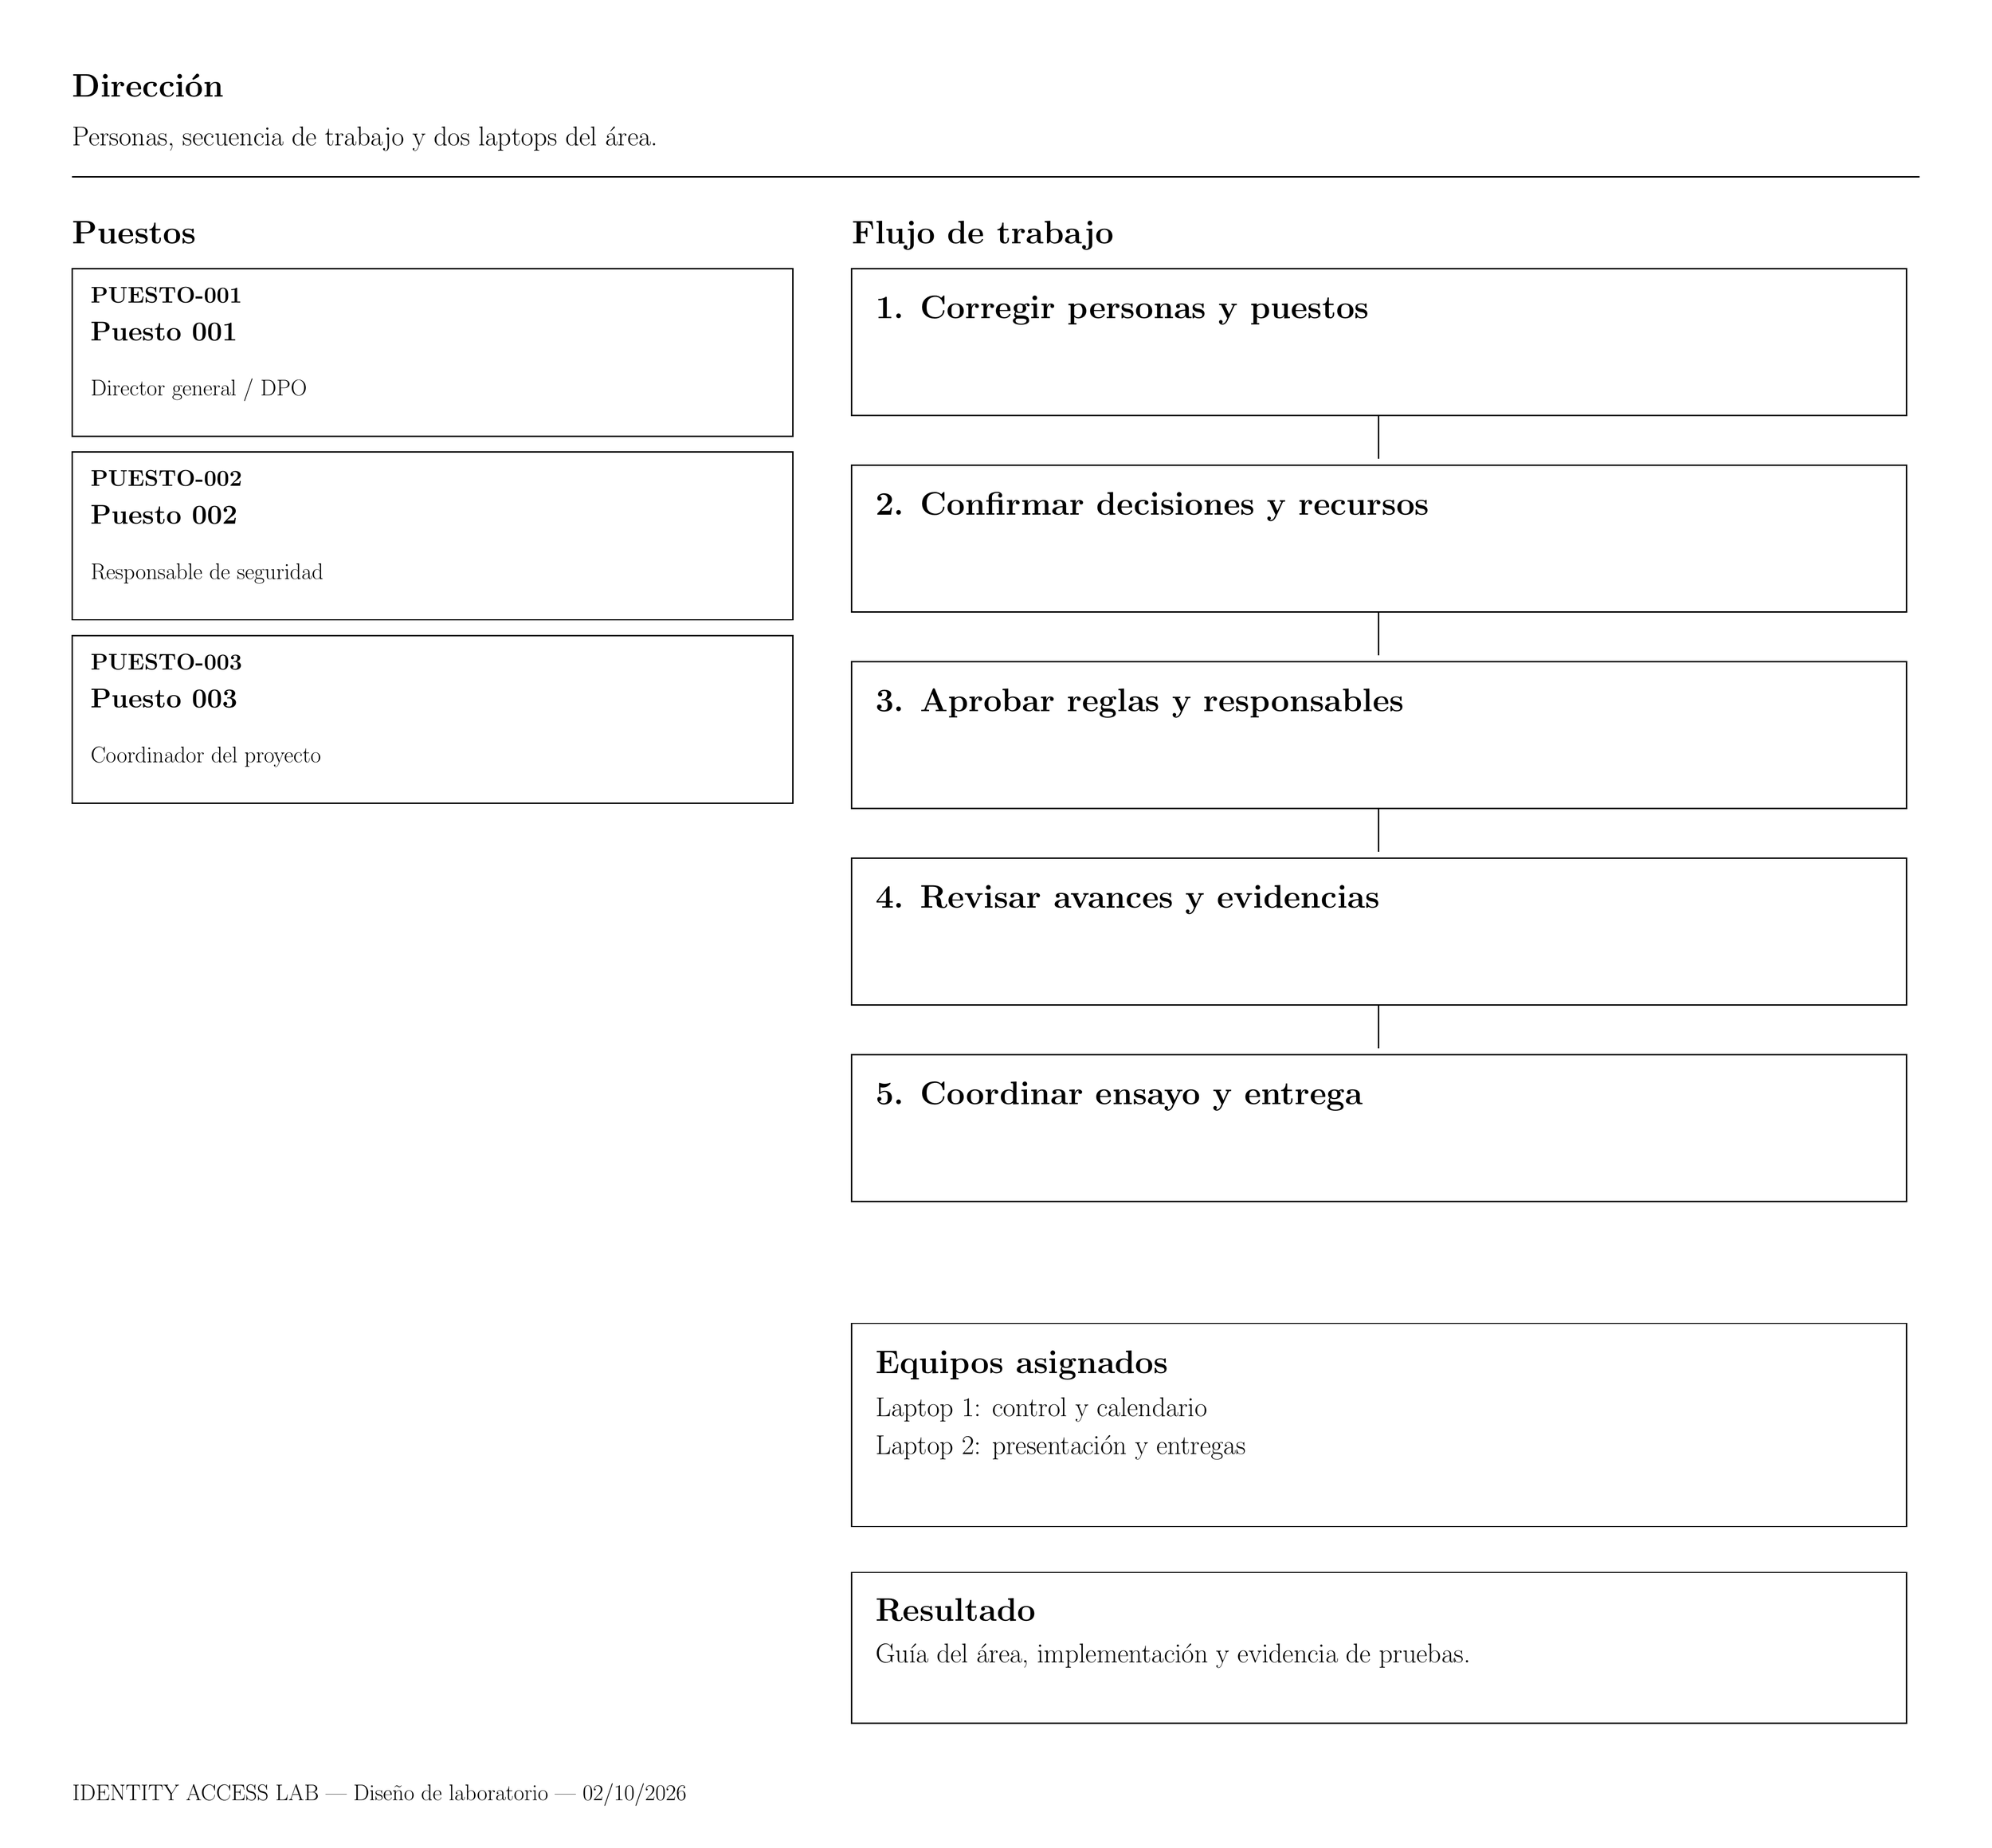
\begin{tikzpicture}[x=1pt,y=-1pt]
\path[use as bounding box] (0,0) rectangle (1500.0,1390.0);
\node[anchor=base west,inner sep=0pt,font=\fontsize{34.0}{40.8}\selectfont \bfseries ] at (45,64) {Dirección};
\node[anchor=base west,inner sep=0pt,font=\fontsize{21.0}{25.2}\selectfont ] at (45,101) {Personas, secuencia de trabajo y dos laptops del área.};
\draw[line width=1pt] (45,125) -- (1455,125);
\node[anchor=base west,inner sep=0pt,font=\fontsize{25.0}{30.0}\selectfont \bfseries ] at (45,176) {Puestos};
\node[anchor=base west,inner sep=0pt,font=\fontsize{25.0}{30.0}\selectfont \bfseries ] at (640,176) {Flujo de trabajo};
\draw[line width=1pt] (45.0,195.0) rectangle (595.0,323.0);
\node[anchor=base west,inner sep=0pt,font=\fontsize{18.0}{21.599999999999998}\selectfont \bfseries ] at (59,221) {PUESTO-001};
\node[anchor=base west,inner sep=0pt,font=\fontsize{20.0}{24.0}\selectfont \bfseries ] at (59,250) {Puesto 001};
\node[anchor=base west,inner sep=0pt,font=\fontsize{19.0}{22.8}\selectfont ] at (59,292) {Director general / DPO};
\draw[line width=1pt] (45.0,335.0) rectangle (595.0,463.0);
\node[anchor=base west,inner sep=0pt,font=\fontsize{18.0}{21.599999999999998}\selectfont \bfseries ] at (59,361) {PUESTO-002};
\node[anchor=base west,inner sep=0pt,font=\fontsize{20.0}{24.0}\selectfont \bfseries ] at (59,390) {Puesto 002};
\node[anchor=base west,inner sep=0pt,font=\fontsize{19.0}{22.8}\selectfont ] at (59,432) {Responsable de seguridad};
\draw[line width=1pt] (45.0,475.0) rectangle (595.0,603.0);
\node[anchor=base west,inner sep=0pt,font=\fontsize{18.0}{21.599999999999998}\selectfont \bfseries ] at (59,501) {PUESTO-003};
\node[anchor=base west,inner sep=0pt,font=\fontsize{20.0}{24.0}\selectfont \bfseries ] at (59,530) {Puesto 003};
\node[anchor=base west,inner sep=0pt,font=\fontsize{19.0}{22.8}\selectfont ] at (59,572) {Coordinador del proyecto};
\draw[line width=1pt] (640.0,195.0) rectangle (1445.0,307.0);
\node[anchor=base west,inner sep=0pt,font=\fontsize{24.0}{28.799999999999997}\selectfont \bfseries ] at (658,233) {1. Corregir personas y puestos};
\draw[line width=1pt] (1042,307) -- (1042,340);
\draw[line width=1pt] (640.0,345.0) rectangle (1445.0,457.0);
\node[anchor=base west,inner sep=0pt,font=\fontsize{24.0}{28.799999999999997}\selectfont \bfseries ] at (658,383) {2. Confirmar decisiones y recursos};
\draw[line width=1pt] (1042,457) -- (1042,490);
\draw[line width=1pt] (640.0,495.0) rectangle (1445.0,607.0);
\node[anchor=base west,inner sep=0pt,font=\fontsize{24.0}{28.799999999999997}\selectfont \bfseries ] at (658,533) {3. Aprobar reglas y responsables};
\draw[line width=1pt] (1042,607) -- (1042,640);
\draw[line width=1pt] (640.0,645.0) rectangle (1445.0,757.0);
\node[anchor=base west,inner sep=0pt,font=\fontsize{24.0}{28.799999999999997}\selectfont \bfseries ] at (658,683) {4. Revisar avances y evidencias};
\draw[line width=1pt] (1042,757) -- (1042,790);
\draw[line width=1pt] (640.0,795.0) rectangle (1445.0,907.0);
\node[anchor=base west,inner sep=0pt,font=\fontsize{24.0}{28.799999999999997}\selectfont \bfseries ] at (658,833) {5. Coordinar ensayo y entrega};
\draw[line width=1pt] (640.0,1000.0) rectangle (1445.0,1155.0);
\node[anchor=base west,inner sep=0pt,font=\fontsize{24.0}{28.799999999999997}\selectfont \bfseries ] at (658,1038) {Equipos asignados};
\node[anchor=base west,inner sep=0pt,font=\fontsize{22.0}{26.4}\selectfont ] at (658,1071) {Laptop 1: control y calendario};
\node[anchor=base west,inner sep=0pt,font=\fontsize{22.0}{26.4}\selectfont ] at (658,1100) {Laptop 2: presentación y entregas};
\draw[line width=1pt] (640.0,1190.0) rectangle (1445.0,1305.0);
\node[anchor=base west,inner sep=0pt,font=\fontsize{23.0}{27.599999999999998}\selectfont \bfseries ] at (658,1227) {Resultado};
\node[anchor=base west,inner sep=0pt,font=\fontsize{21.0}{25.2}\selectfont ] at (658,1259) {Guía del área, implementación y evidencia de pruebas.};
\node[anchor=base west,inner sep=0pt,font=\fontsize{18.0}{21.599999999999998}\selectfont ] at (45,1364) {IDENTITY ACCESS LAB | Diseño de laboratorio | 02/10/2026};
\end{tikzpicture}}
\clearpage
\noindent\resizebox{\textwidth}{!}{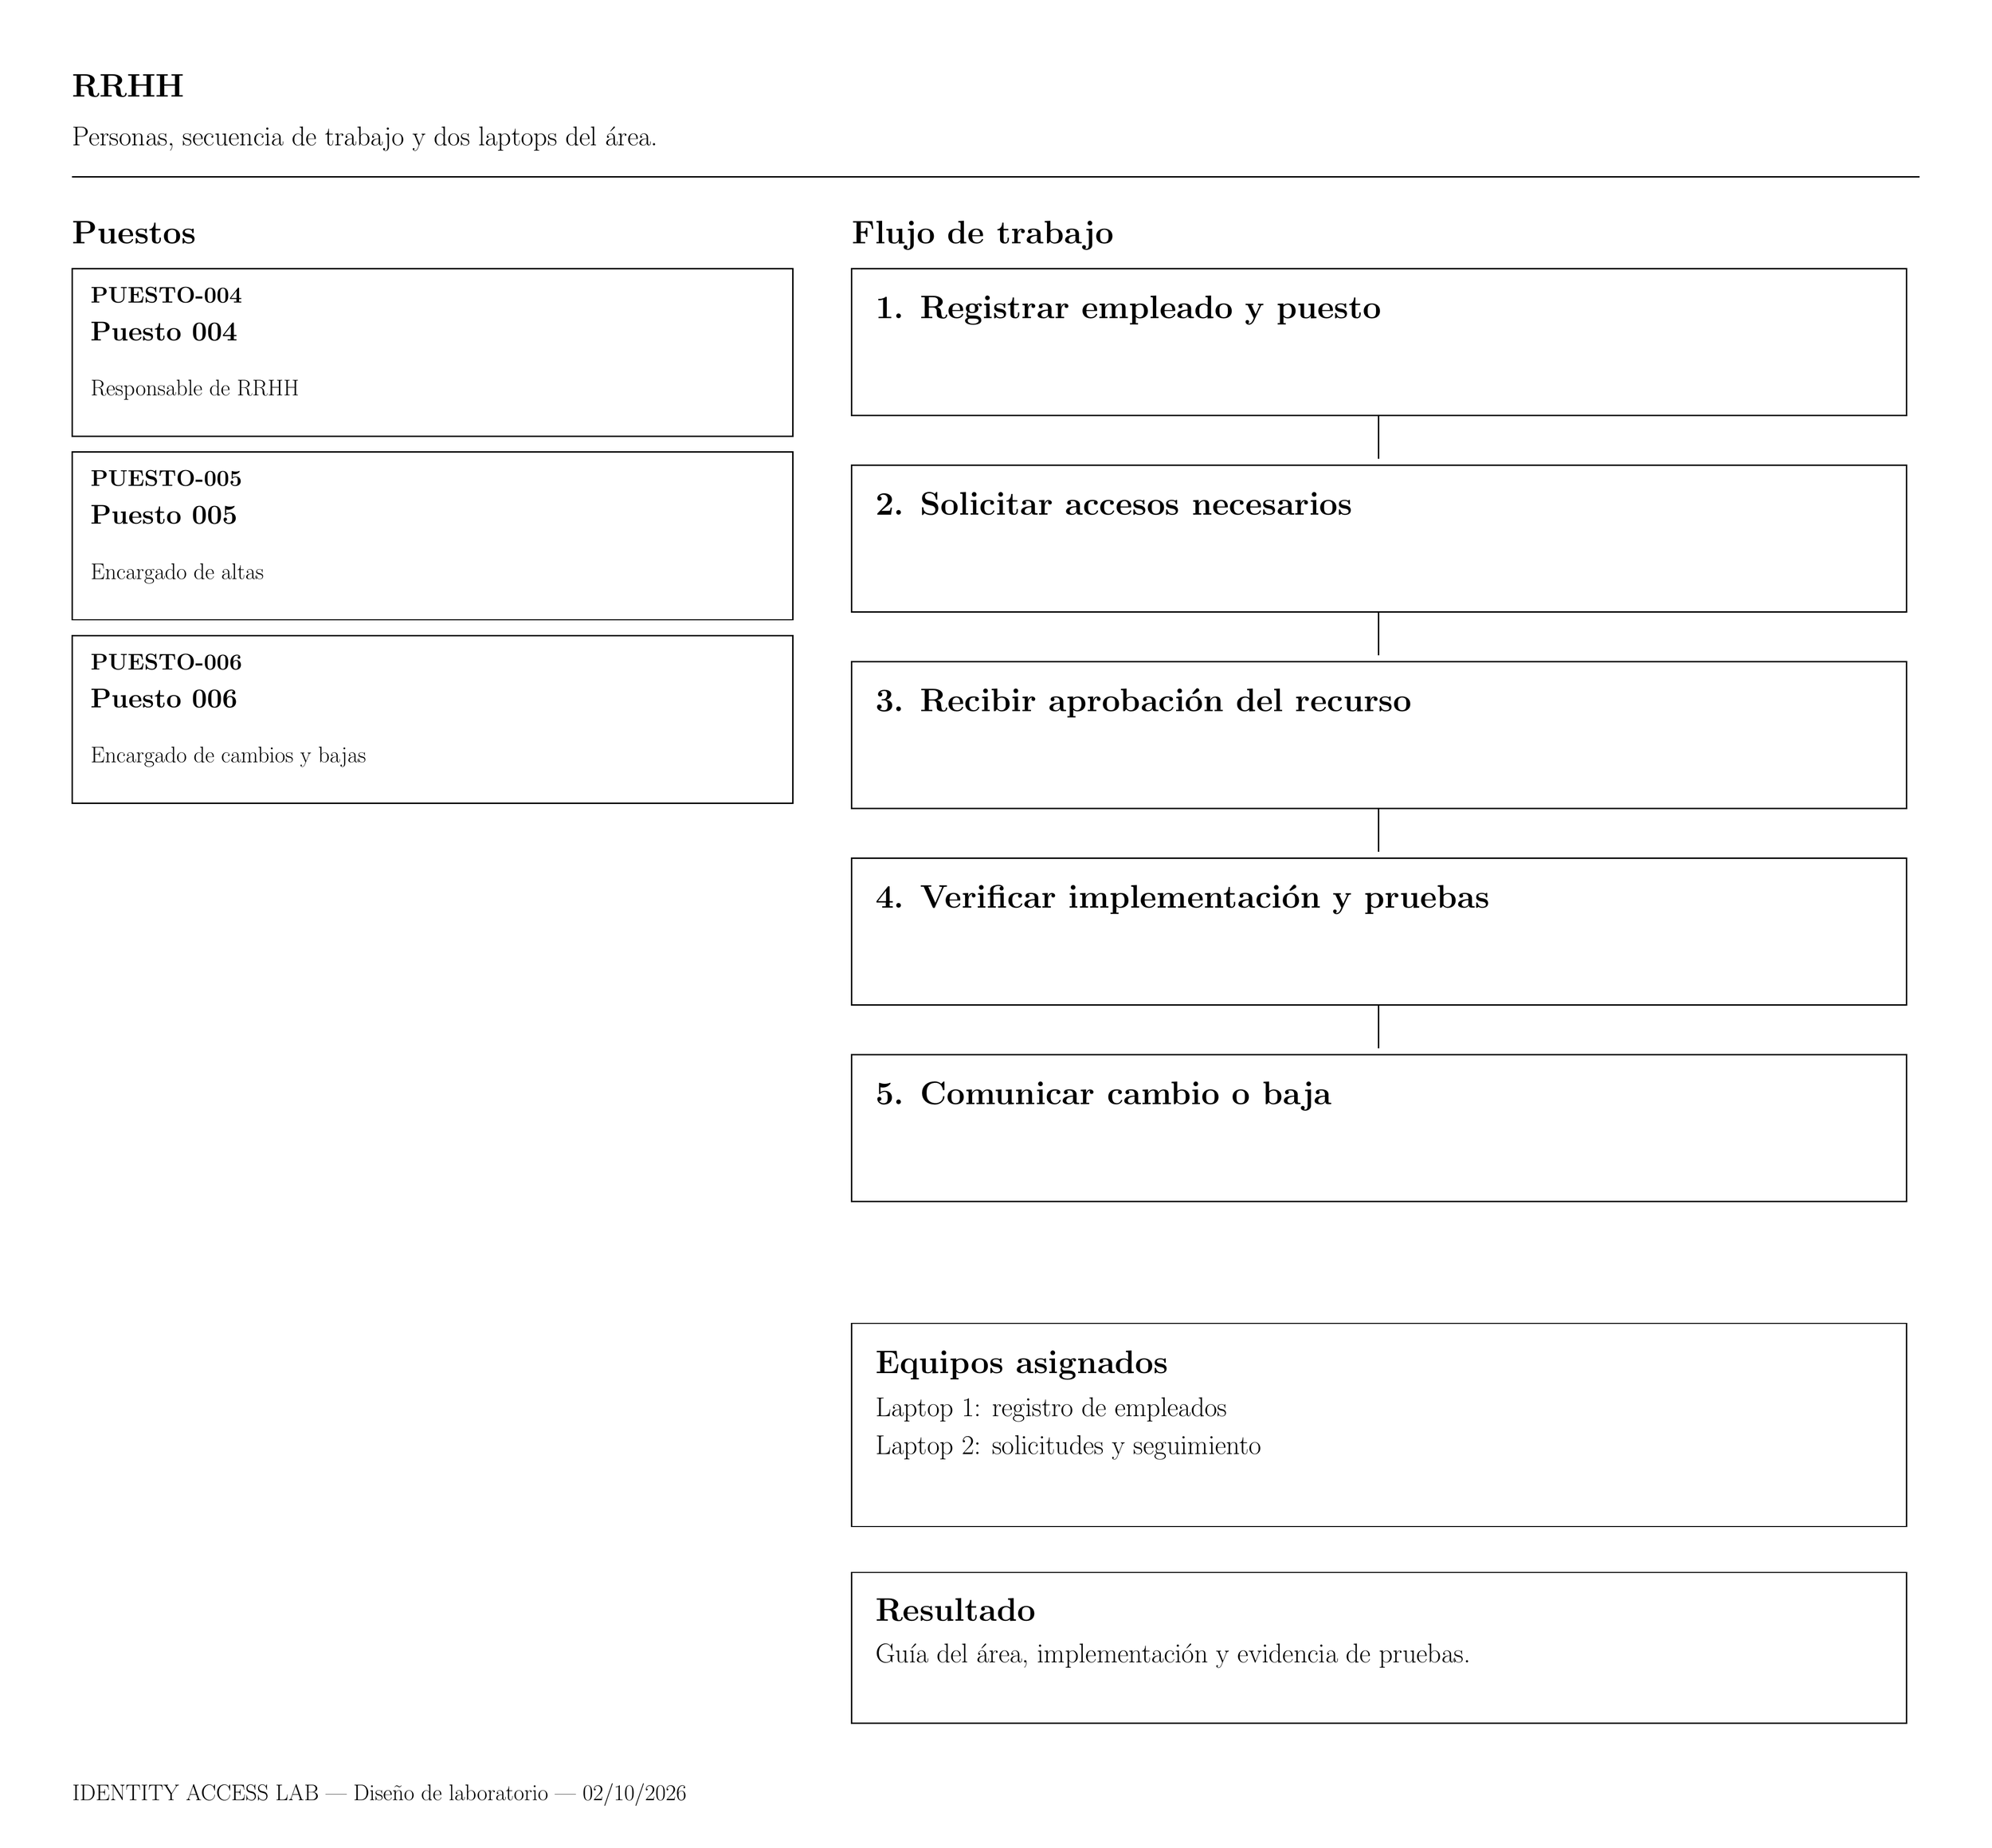
\begin{tikzpicture}[x=1pt,y=-1pt]
\path[use as bounding box] (0,0) rectangle (1500.0,1390.0);
\node[anchor=base west,inner sep=0pt,font=\fontsize{34.0}{40.8}\selectfont \bfseries ] at (45,64) {RRHH};
\node[anchor=base west,inner sep=0pt,font=\fontsize{21.0}{25.2}\selectfont ] at (45,101) {Personas, secuencia de trabajo y dos laptops del área.};
\draw[line width=1pt] (45,125) -- (1455,125);
\node[anchor=base west,inner sep=0pt,font=\fontsize{25.0}{30.0}\selectfont \bfseries ] at (45,176) {Puestos};
\node[anchor=base west,inner sep=0pt,font=\fontsize{25.0}{30.0}\selectfont \bfseries ] at (640,176) {Flujo de trabajo};
\draw[line width=1pt] (45.0,195.0) rectangle (595.0,323.0);
\node[anchor=base west,inner sep=0pt,font=\fontsize{18.0}{21.599999999999998}\selectfont \bfseries ] at (59,221) {PUESTO-004};
\node[anchor=base west,inner sep=0pt,font=\fontsize{20.0}{24.0}\selectfont \bfseries ] at (59,250) {Puesto 004};
\node[anchor=base west,inner sep=0pt,font=\fontsize{19.0}{22.8}\selectfont ] at (59,292) {Responsable de RRHH};
\draw[line width=1pt] (45.0,335.0) rectangle (595.0,463.0);
\node[anchor=base west,inner sep=0pt,font=\fontsize{18.0}{21.599999999999998}\selectfont \bfseries ] at (59,361) {PUESTO-005};
\node[anchor=base west,inner sep=0pt,font=\fontsize{20.0}{24.0}\selectfont \bfseries ] at (59,390) {Puesto 005};
\node[anchor=base west,inner sep=0pt,font=\fontsize{19.0}{22.8}\selectfont ] at (59,432) {Encargado de altas};
\draw[line width=1pt] (45.0,475.0) rectangle (595.0,603.0);
\node[anchor=base west,inner sep=0pt,font=\fontsize{18.0}{21.599999999999998}\selectfont \bfseries ] at (59,501) {PUESTO-006};
\node[anchor=base west,inner sep=0pt,font=\fontsize{20.0}{24.0}\selectfont \bfseries ] at (59,530) {Puesto 006};
\node[anchor=base west,inner sep=0pt,font=\fontsize{19.0}{22.8}\selectfont ] at (59,572) {Encargado de cambios y bajas};
\draw[line width=1pt] (640.0,195.0) rectangle (1445.0,307.0);
\node[anchor=base west,inner sep=0pt,font=\fontsize{24.0}{28.799999999999997}\selectfont \bfseries ] at (658,233) {1. Registrar empleado y puesto};
\draw[line width=1pt] (1042,307) -- (1042,340);
\draw[line width=1pt] (640.0,345.0) rectangle (1445.0,457.0);
\node[anchor=base west,inner sep=0pt,font=\fontsize{24.0}{28.799999999999997}\selectfont \bfseries ] at (658,383) {2. Solicitar accesos necesarios};
\draw[line width=1pt] (1042,457) -- (1042,490);
\draw[line width=1pt] (640.0,495.0) rectangle (1445.0,607.0);
\node[anchor=base west,inner sep=0pt,font=\fontsize{24.0}{28.799999999999997}\selectfont \bfseries ] at (658,533) {3. Recibir aprobación del recurso};
\draw[line width=1pt] (1042,607) -- (1042,640);
\draw[line width=1pt] (640.0,645.0) rectangle (1445.0,757.0);
\node[anchor=base west,inner sep=0pt,font=\fontsize{24.0}{28.799999999999997}\selectfont \bfseries ] at (658,683) {4. Verificar implementación y pruebas};
\draw[line width=1pt] (1042,757) -- (1042,790);
\draw[line width=1pt] (640.0,795.0) rectangle (1445.0,907.0);
\node[anchor=base west,inner sep=0pt,font=\fontsize{24.0}{28.799999999999997}\selectfont \bfseries ] at (658,833) {5. Comunicar cambio o baja};
\draw[line width=1pt] (640.0,1000.0) rectangle (1445.0,1155.0);
\node[anchor=base west,inner sep=0pt,font=\fontsize{24.0}{28.799999999999997}\selectfont \bfseries ] at (658,1038) {Equipos asignados};
\node[anchor=base west,inner sep=0pt,font=\fontsize{22.0}{26.4}\selectfont ] at (658,1071) {Laptop 1: registro de empleados};
\node[anchor=base west,inner sep=0pt,font=\fontsize{22.0}{26.4}\selectfont ] at (658,1100) {Laptop 2: solicitudes y seguimiento};
\draw[line width=1pt] (640.0,1190.0) rectangle (1445.0,1305.0);
\node[anchor=base west,inner sep=0pt,font=\fontsize{23.0}{27.599999999999998}\selectfont \bfseries ] at (658,1227) {Resultado};
\node[anchor=base west,inner sep=0pt,font=\fontsize{21.0}{25.2}\selectfont ] at (658,1259) {Guía del área, implementación y evidencia de pruebas.};
\node[anchor=base west,inner sep=0pt,font=\fontsize{18.0}{21.599999999999998}\selectfont ] at (45,1364) {IDENTITY ACCESS LAB | Diseño de laboratorio | 02/10/2026};
\end{tikzpicture}}
\clearpage
\noindent\resizebox{\textwidth}{!}{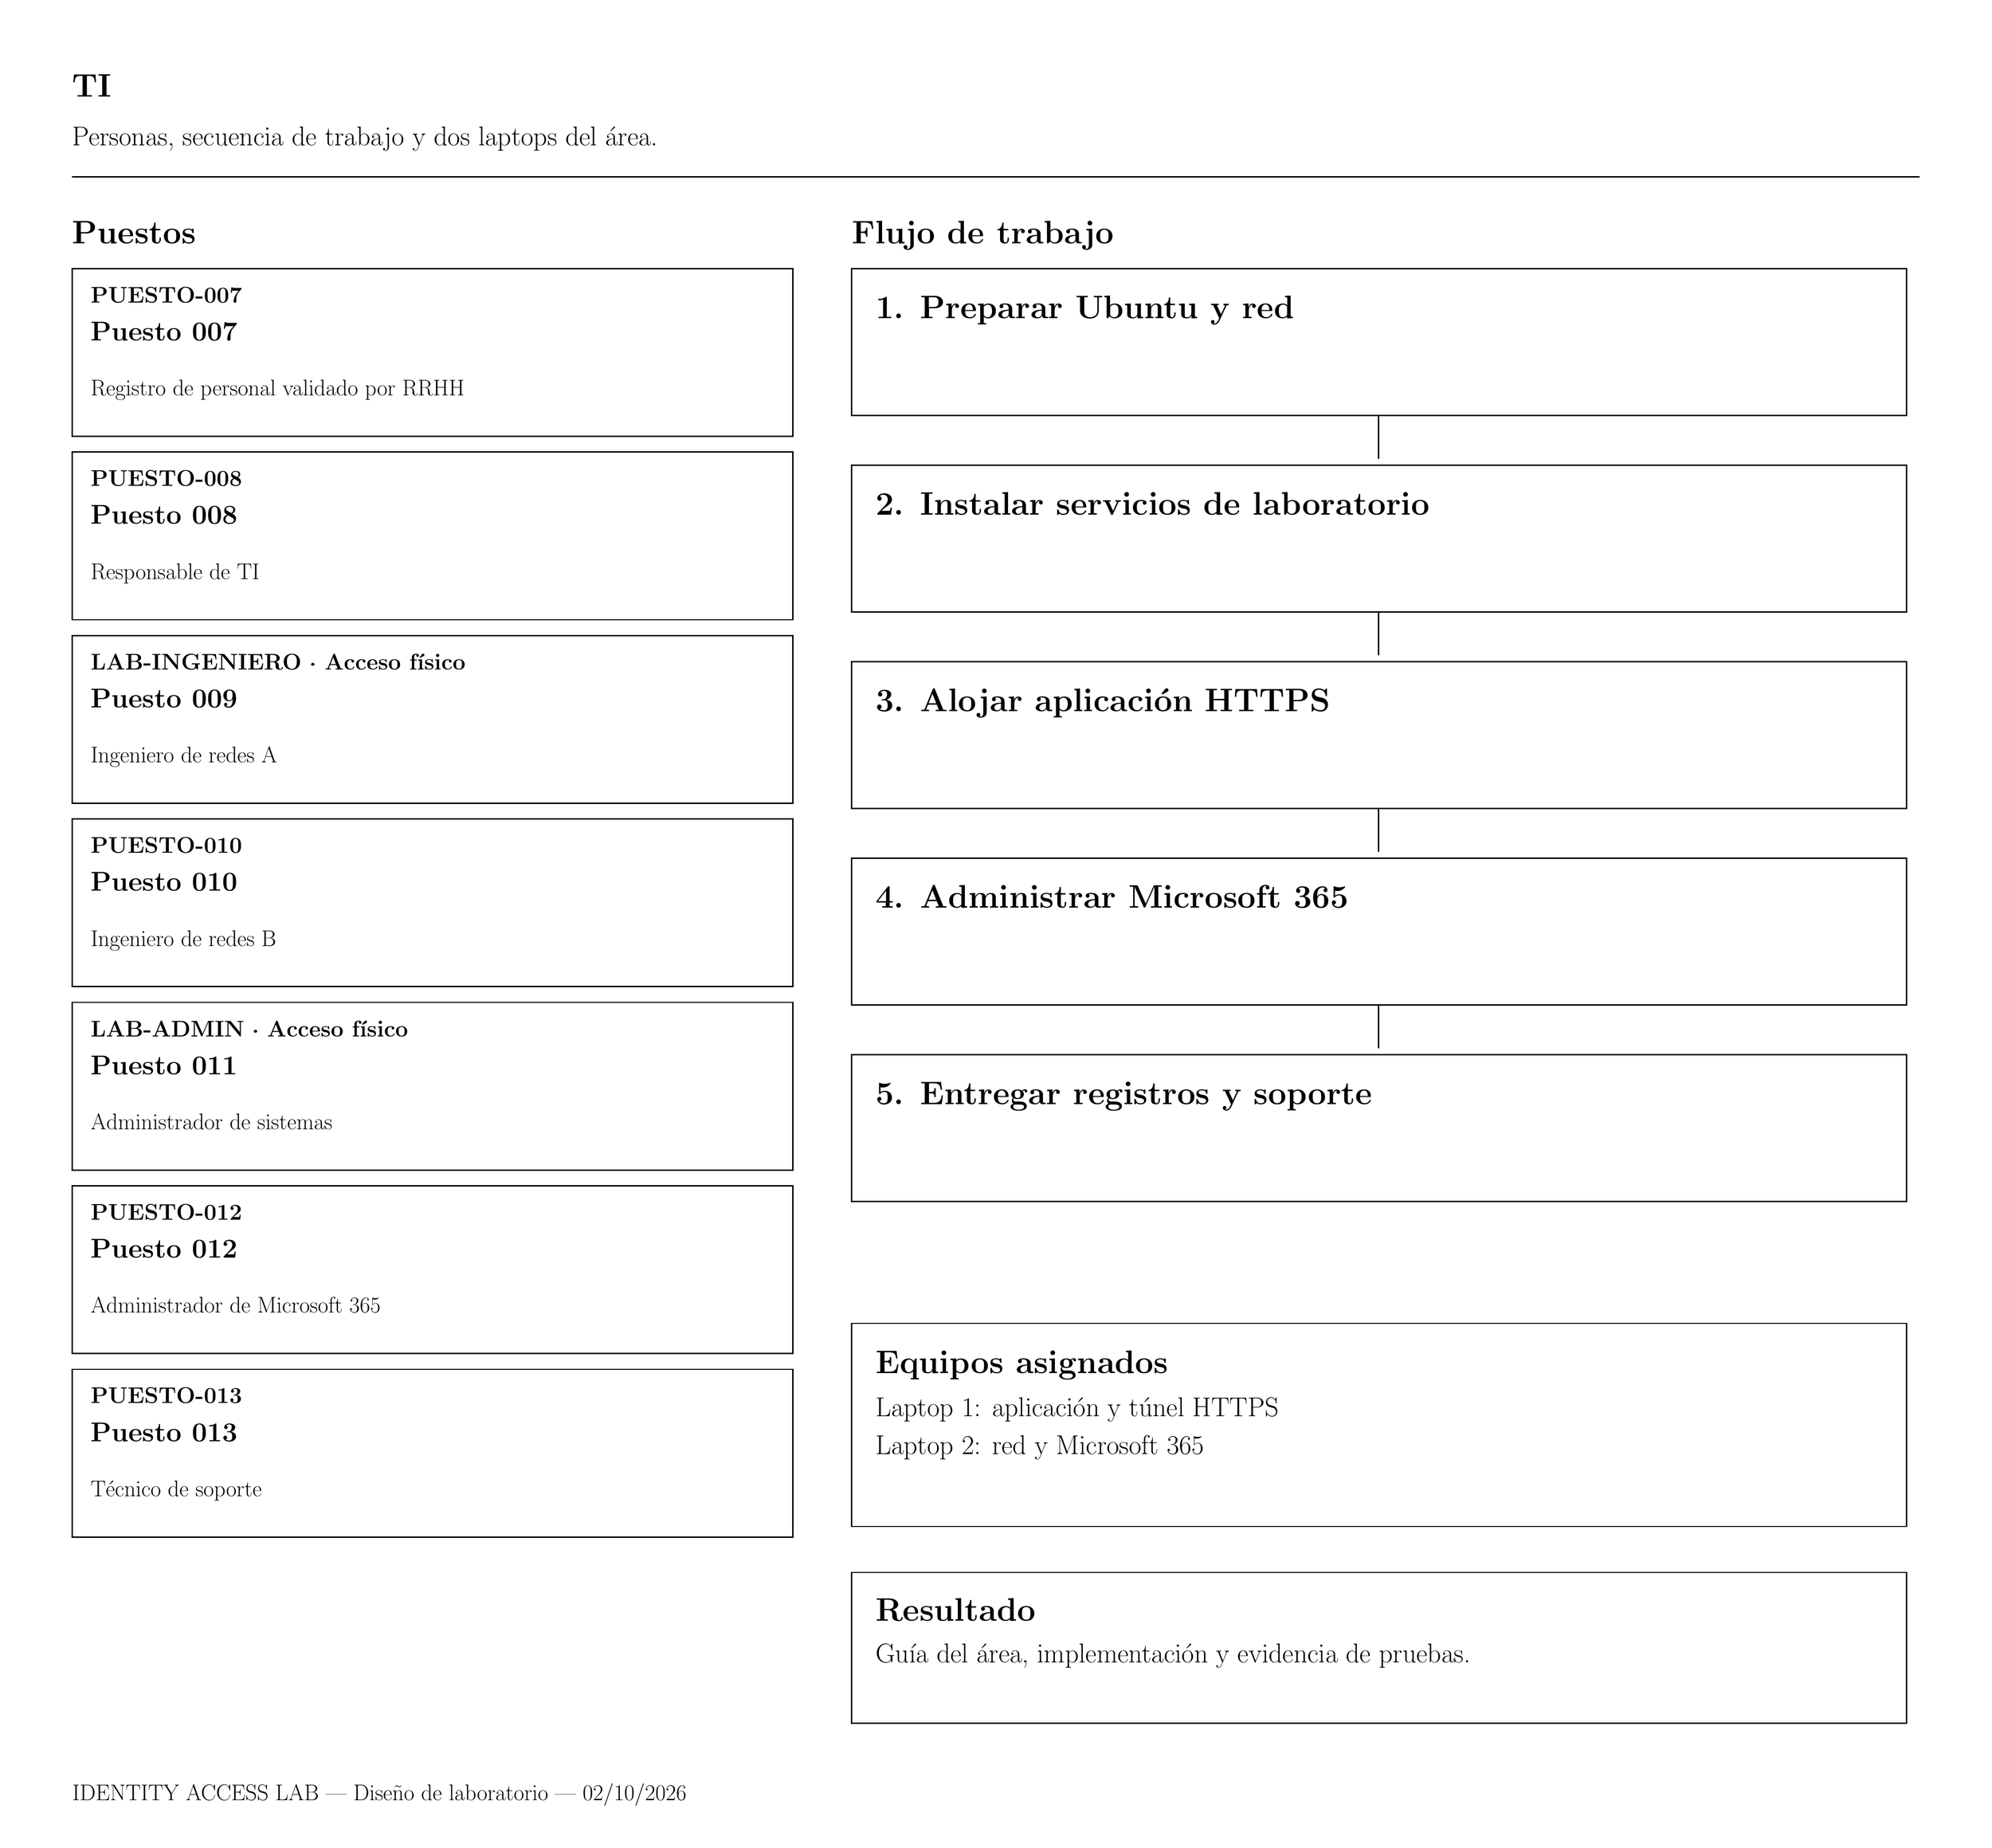
\begin{tikzpicture}[x=1pt,y=-1pt]
\path[use as bounding box] (0,0) rectangle (1500.0,1390.0);
\node[anchor=base west,inner sep=0pt,font=\fontsize{34.0}{40.8}\selectfont \bfseries ] at (45,64) {TI};
\node[anchor=base west,inner sep=0pt,font=\fontsize{21.0}{25.2}\selectfont ] at (45,101) {Personas, secuencia de trabajo y dos laptops del área.};
\draw[line width=1pt] (45,125) -- (1455,125);
\node[anchor=base west,inner sep=0pt,font=\fontsize{25.0}{30.0}\selectfont \bfseries ] at (45,176) {Puestos};
\node[anchor=base west,inner sep=0pt,font=\fontsize{25.0}{30.0}\selectfont \bfseries ] at (640,176) {Flujo de trabajo};
\draw[line width=1pt] (45.0,195.0) rectangle (595.0,323.0);
\node[anchor=base west,inner sep=0pt,font=\fontsize{18.0}{21.599999999999998}\selectfont \bfseries ] at (59,221) {PUESTO-007};
\node[anchor=base west,inner sep=0pt,font=\fontsize{20.0}{24.0}\selectfont \bfseries ] at (59,250) {Puesto 007};
\node[anchor=base west,inner sep=0pt,font=\fontsize{19.0}{22.8}\selectfont ] at (59,292) {Registro de personal validado por RRHH};
\draw[line width=1pt] (45.0,335.0) rectangle (595.0,463.0);
\node[anchor=base west,inner sep=0pt,font=\fontsize{18.0}{21.599999999999998}\selectfont \bfseries ] at (59,361) {PUESTO-008};
\node[anchor=base west,inner sep=0pt,font=\fontsize{20.0}{24.0}\selectfont \bfseries ] at (59,390) {Puesto 008};
\node[anchor=base west,inner sep=0pt,font=\fontsize{19.0}{22.8}\selectfont ] at (59,432) {Responsable de TI};
\draw[line width=1pt] (45.0,475.0) rectangle (595.0,603.0);
\node[anchor=base west,inner sep=0pt,font=\fontsize{18.0}{21.599999999999998}\selectfont \bfseries ] at (59,501) {LAB-INGENIERO · Acceso físico};
\node[anchor=base west,inner sep=0pt,font=\fontsize{20.0}{24.0}\selectfont \bfseries ] at (59,530) {Puesto 009};
\node[anchor=base west,inner sep=0pt,font=\fontsize{19.0}{22.8}\selectfont ] at (59,572) {Ingeniero de redes A};
\draw[line width=1pt] (45.0,615.0) rectangle (595.0,743.0);
\node[anchor=base west,inner sep=0pt,font=\fontsize{18.0}{21.599999999999998}\selectfont \bfseries ] at (59,641) {PUESTO-010};
\node[anchor=base west,inner sep=0pt,font=\fontsize{20.0}{24.0}\selectfont \bfseries ] at (59,670) {Puesto 010};
\node[anchor=base west,inner sep=0pt,font=\fontsize{19.0}{22.8}\selectfont ] at (59,712) {Ingeniero de redes B};
\draw[line width=1pt] (45.0,755.0) rectangle (595.0,883.0);
\node[anchor=base west,inner sep=0pt,font=\fontsize{18.0}{21.599999999999998}\selectfont \bfseries ] at (59,781) {LAB-ADMIN · Acceso físico};
\node[anchor=base west,inner sep=0pt,font=\fontsize{20.0}{24.0}\selectfont \bfseries ] at (59,810) {Puesto 011};
\node[anchor=base west,inner sep=0pt,font=\fontsize{19.0}{22.8}\selectfont ] at (59,852) {Administrador de sistemas};
\draw[line width=1pt] (45.0,895.0) rectangle (595.0,1023.0);
\node[anchor=base west,inner sep=0pt,font=\fontsize{18.0}{21.599999999999998}\selectfont \bfseries ] at (59,921) {PUESTO-012};
\node[anchor=base west,inner sep=0pt,font=\fontsize{20.0}{24.0}\selectfont \bfseries ] at (59,950) {Puesto 012};
\node[anchor=base west,inner sep=0pt,font=\fontsize{19.0}{22.8}\selectfont ] at (59,992) {Administrador de Microsoft 365};
\draw[line width=1pt] (45.0,1035.0) rectangle (595.0,1163.0);
\node[anchor=base west,inner sep=0pt,font=\fontsize{18.0}{21.599999999999998}\selectfont \bfseries ] at (59,1061) {PUESTO-013};
\node[anchor=base west,inner sep=0pt,font=\fontsize{20.0}{24.0}\selectfont \bfseries ] at (59,1090) {Puesto 013};
\node[anchor=base west,inner sep=0pt,font=\fontsize{19.0}{22.8}\selectfont ] at (59,1132) {Técnico de soporte};
\draw[line width=1pt] (640.0,195.0) rectangle (1445.0,307.0);
\node[anchor=base west,inner sep=0pt,font=\fontsize{24.0}{28.799999999999997}\selectfont \bfseries ] at (658,233) {1. Preparar Ubuntu y red};
\draw[line width=1pt] (1042,307) -- (1042,340);
\draw[line width=1pt] (640.0,345.0) rectangle (1445.0,457.0);
\node[anchor=base west,inner sep=0pt,font=\fontsize{24.0}{28.799999999999997}\selectfont \bfseries ] at (658,383) {2. Instalar servicios de laboratorio};
\draw[line width=1pt] (1042,457) -- (1042,490);
\draw[line width=1pt] (640.0,495.0) rectangle (1445.0,607.0);
\node[anchor=base west,inner sep=0pt,font=\fontsize{24.0}{28.799999999999997}\selectfont \bfseries ] at (658,533) {3. Alojar aplicación HTTPS};
\draw[line width=1pt] (1042,607) -- (1042,640);
\draw[line width=1pt] (640.0,645.0) rectangle (1445.0,757.0);
\node[anchor=base west,inner sep=0pt,font=\fontsize{24.0}{28.799999999999997}\selectfont \bfseries ] at (658,683) {4. Administrar Microsoft 365};
\draw[line width=1pt] (1042,757) -- (1042,790);
\draw[line width=1pt] (640.0,795.0) rectangle (1445.0,907.0);
\node[anchor=base west,inner sep=0pt,font=\fontsize{24.0}{28.799999999999997}\selectfont \bfseries ] at (658,833) {5. Entregar registros y soporte};
\draw[line width=1pt] (640.0,1000.0) rectangle (1445.0,1155.0);
\node[anchor=base west,inner sep=0pt,font=\fontsize{24.0}{28.799999999999997}\selectfont \bfseries ] at (658,1038) {Equipos asignados};
\node[anchor=base west,inner sep=0pt,font=\fontsize{22.0}{26.4}\selectfont ] at (658,1071) {Laptop 1: aplicación y túnel HTTPS};
\node[anchor=base west,inner sep=0pt,font=\fontsize{22.0}{26.4}\selectfont ] at (658,1100) {Laptop 2: red y Microsoft 365};
\draw[line width=1pt] (640.0,1190.0) rectangle (1445.0,1305.0);
\node[anchor=base west,inner sep=0pt,font=\fontsize{23.0}{27.599999999999998}\selectfont \bfseries ] at (658,1227) {Resultado};
\node[anchor=base west,inner sep=0pt,font=\fontsize{21.0}{25.2}\selectfont ] at (658,1259) {Guía del área, implementación y evidencia de pruebas.};
\node[anchor=base west,inner sep=0pt,font=\fontsize{18.0}{21.599999999999998}\selectfont ] at (45,1364) {IDENTITY ACCESS LAB | Diseño de laboratorio | 02/10/2026};
\end{tikzpicture}}
\clearpage
\noindent\resizebox{\textwidth}{!}{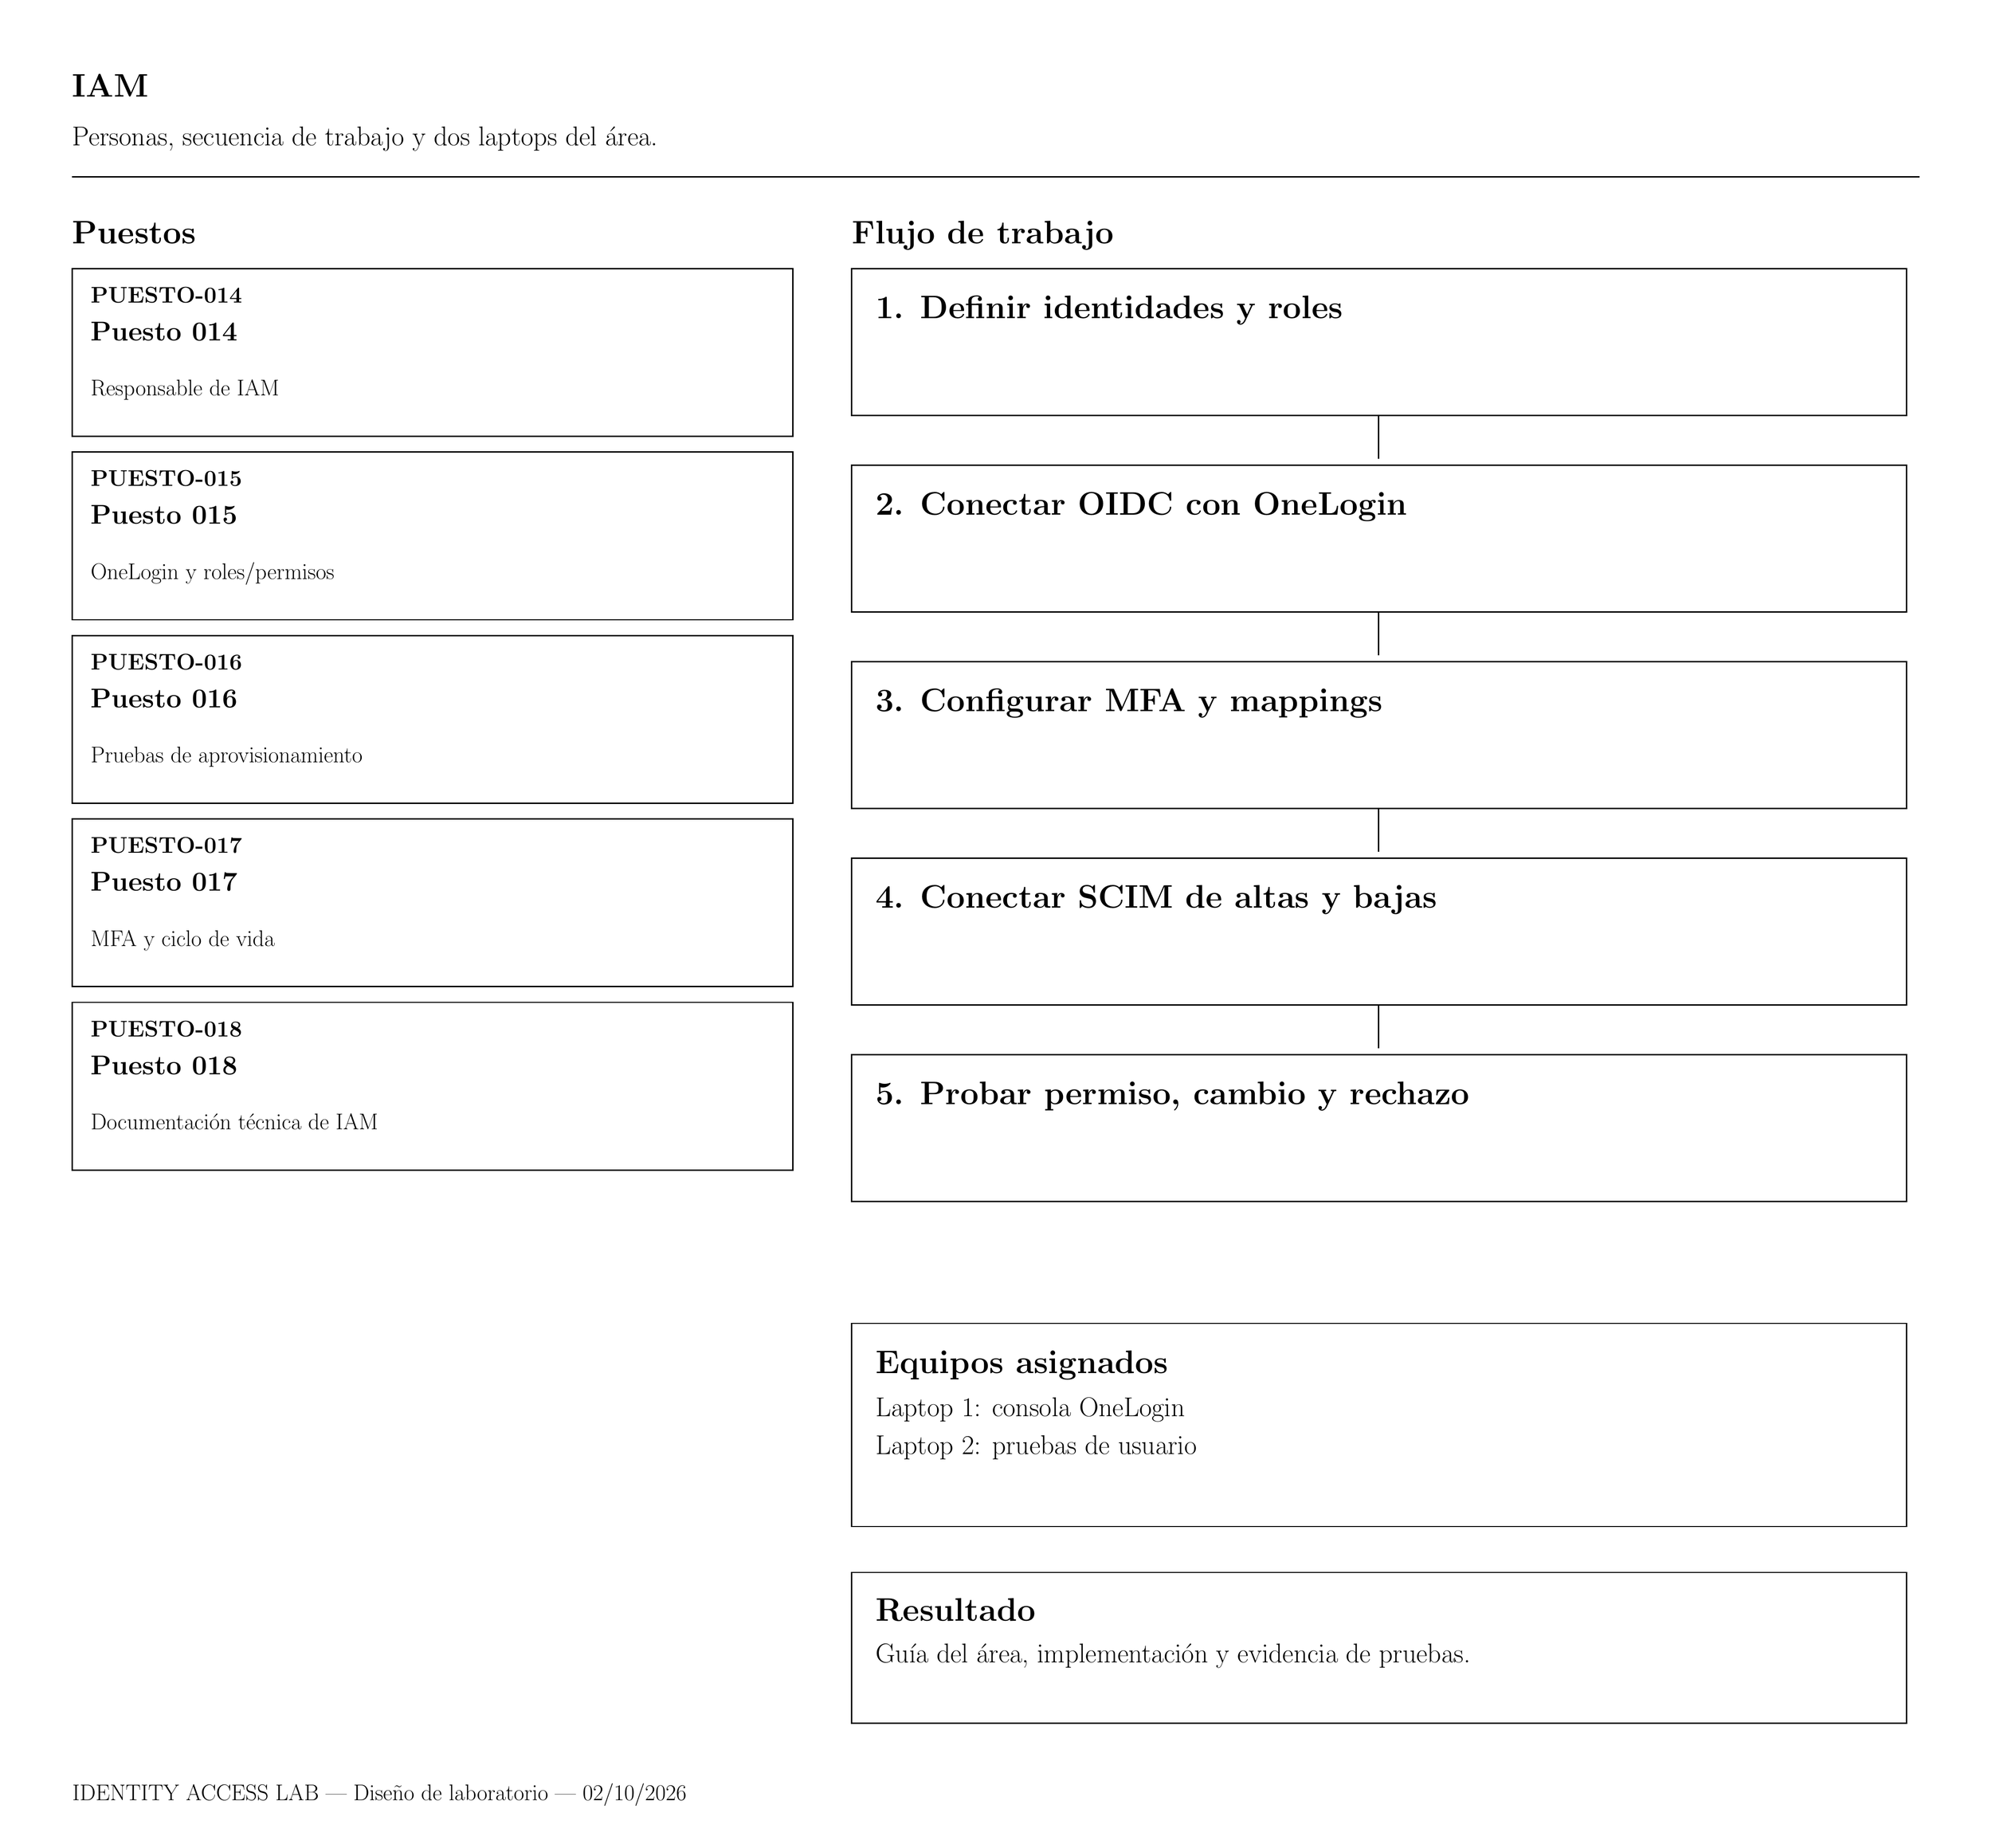
\begin{tikzpicture}[x=1pt,y=-1pt]
\path[use as bounding box] (0,0) rectangle (1500.0,1390.0);
\node[anchor=base west,inner sep=0pt,font=\fontsize{34.0}{40.8}\selectfont \bfseries ] at (45,64) {IAM};
\node[anchor=base west,inner sep=0pt,font=\fontsize{21.0}{25.2}\selectfont ] at (45,101) {Personas, secuencia de trabajo y dos laptops del área.};
\draw[line width=1pt] (45,125) -- (1455,125);
\node[anchor=base west,inner sep=0pt,font=\fontsize{25.0}{30.0}\selectfont \bfseries ] at (45,176) {Puestos};
\node[anchor=base west,inner sep=0pt,font=\fontsize{25.0}{30.0}\selectfont \bfseries ] at (640,176) {Flujo de trabajo};
\draw[line width=1pt] (45.0,195.0) rectangle (595.0,323.0);
\node[anchor=base west,inner sep=0pt,font=\fontsize{18.0}{21.599999999999998}\selectfont \bfseries ] at (59,221) {PUESTO-014};
\node[anchor=base west,inner sep=0pt,font=\fontsize{20.0}{24.0}\selectfont \bfseries ] at (59,250) {Puesto 014};
\node[anchor=base west,inner sep=0pt,font=\fontsize{19.0}{22.8}\selectfont ] at (59,292) {Responsable de IAM};
\draw[line width=1pt] (45.0,335.0) rectangle (595.0,463.0);
\node[anchor=base west,inner sep=0pt,font=\fontsize{18.0}{21.599999999999998}\selectfont \bfseries ] at (59,361) {PUESTO-015};
\node[anchor=base west,inner sep=0pt,font=\fontsize{20.0}{24.0}\selectfont \bfseries ] at (59,390) {Puesto 015};
\node[anchor=base west,inner sep=0pt,font=\fontsize{19.0}{22.8}\selectfont ] at (59,432) {OneLogin y roles/permisos};
\draw[line width=1pt] (45.0,475.0) rectangle (595.0,603.0);
\node[anchor=base west,inner sep=0pt,font=\fontsize{18.0}{21.599999999999998}\selectfont \bfseries ] at (59,501) {PUESTO-016};
\node[anchor=base west,inner sep=0pt,font=\fontsize{20.0}{24.0}\selectfont \bfseries ] at (59,530) {Puesto 016};
\node[anchor=base west,inner sep=0pt,font=\fontsize{19.0}{22.8}\selectfont ] at (59,572) {Pruebas de aprovisionamiento};
\draw[line width=1pt] (45.0,615.0) rectangle (595.0,743.0);
\node[anchor=base west,inner sep=0pt,font=\fontsize{18.0}{21.599999999999998}\selectfont \bfseries ] at (59,641) {PUESTO-017};
\node[anchor=base west,inner sep=0pt,font=\fontsize{20.0}{24.0}\selectfont \bfseries ] at (59,670) {Puesto 017};
\node[anchor=base west,inner sep=0pt,font=\fontsize{19.0}{22.8}\selectfont ] at (59,712) {MFA y ciclo de vida};
\draw[line width=1pt] (45.0,755.0) rectangle (595.0,883.0);
\node[anchor=base west,inner sep=0pt,font=\fontsize{18.0}{21.599999999999998}\selectfont \bfseries ] at (59,781) {PUESTO-018};
\node[anchor=base west,inner sep=0pt,font=\fontsize{20.0}{24.0}\selectfont \bfseries ] at (59,810) {Puesto 018};
\node[anchor=base west,inner sep=0pt,font=\fontsize{19.0}{22.8}\selectfont ] at (59,852) {Documentación técnica de IAM};
\draw[line width=1pt] (640.0,195.0) rectangle (1445.0,307.0);
\node[anchor=base west,inner sep=0pt,font=\fontsize{24.0}{28.799999999999997}\selectfont \bfseries ] at (658,233) {1. Definir identidades y roles};
\draw[line width=1pt] (1042,307) -- (1042,340);
\draw[line width=1pt] (640.0,345.0) rectangle (1445.0,457.0);
\node[anchor=base west,inner sep=0pt,font=\fontsize{24.0}{28.799999999999997}\selectfont \bfseries ] at (658,383) {2. Conectar OIDC con OneLogin};
\draw[line width=1pt] (1042,457) -- (1042,490);
\draw[line width=1pt] (640.0,495.0) rectangle (1445.0,607.0);
\node[anchor=base west,inner sep=0pt,font=\fontsize{24.0}{28.799999999999997}\selectfont \bfseries ] at (658,533) {3. Configurar MFA y mappings};
\draw[line width=1pt] (1042,607) -- (1042,640);
\draw[line width=1pt] (640.0,645.0) rectangle (1445.0,757.0);
\node[anchor=base west,inner sep=0pt,font=\fontsize{24.0}{28.799999999999997}\selectfont \bfseries ] at (658,683) {4. Conectar SCIM de altas y bajas};
\draw[line width=1pt] (1042,757) -- (1042,790);
\draw[line width=1pt] (640.0,795.0) rectangle (1445.0,907.0);
\node[anchor=base west,inner sep=0pt,font=\fontsize{24.0}{28.799999999999997}\selectfont \bfseries ] at (658,833) {5. Probar permiso, cambio y rechazo};
\draw[line width=1pt] (640.0,1000.0) rectangle (1445.0,1155.0);
\node[anchor=base west,inner sep=0pt,font=\fontsize{24.0}{28.799999999999997}\selectfont \bfseries ] at (658,1038) {Equipos asignados};
\node[anchor=base west,inner sep=0pt,font=\fontsize{22.0}{26.4}\selectfont ] at (658,1071) {Laptop 1: consola OneLogin};
\node[anchor=base west,inner sep=0pt,font=\fontsize{22.0}{26.4}\selectfont ] at (658,1100) {Laptop 2: pruebas de usuario};
\draw[line width=1pt] (640.0,1190.0) rectangle (1445.0,1305.0);
\node[anchor=base west,inner sep=0pt,font=\fontsize{23.0}{27.599999999999998}\selectfont \bfseries ] at (658,1227) {Resultado};
\node[anchor=base west,inner sep=0pt,font=\fontsize{21.0}{25.2}\selectfont ] at (658,1259) {Guía del área, implementación y evidencia de pruebas.};
\node[anchor=base west,inner sep=0pt,font=\fontsize{18.0}{21.599999999999998}\selectfont ] at (45,1364) {IDENTITY ACCESS LAB | Diseño de laboratorio | 02/10/2026};
\end{tikzpicture}}
\clearpage
\noindent\resizebox{\textwidth}{!}{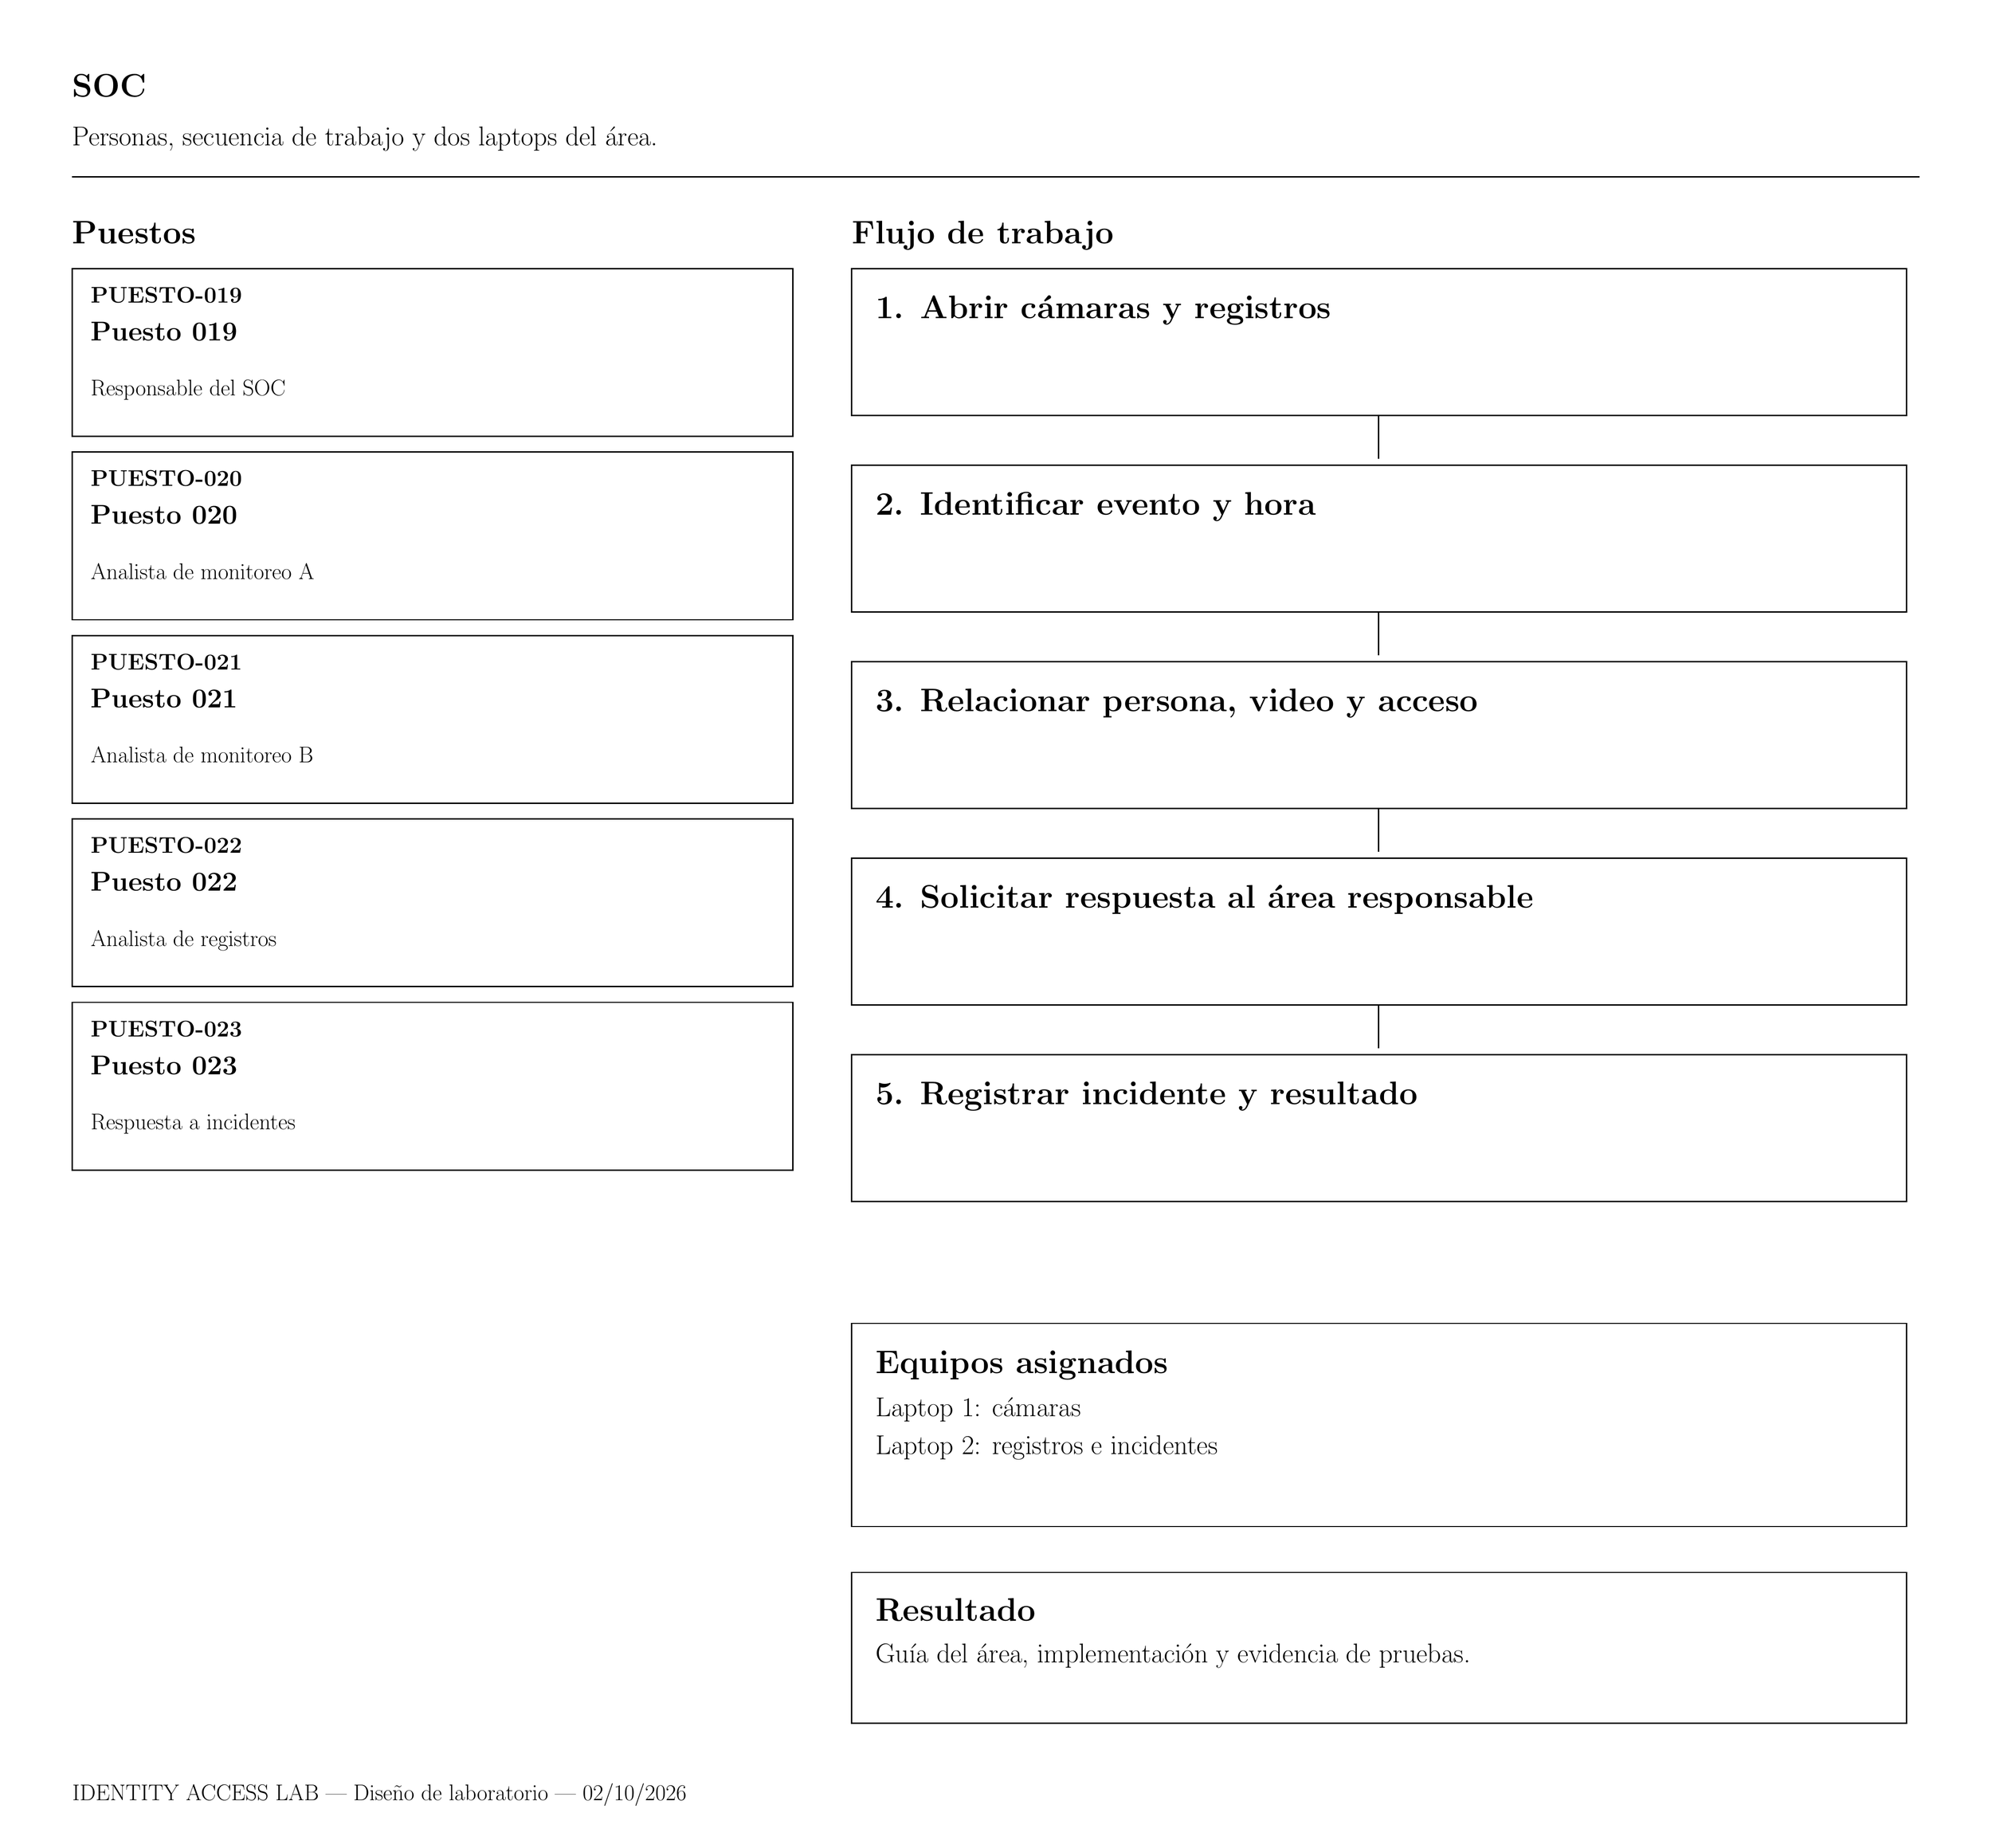
\begin{tikzpicture}[x=1pt,y=-1pt]
\path[use as bounding box] (0,0) rectangle (1500.0,1390.0);
\node[anchor=base west,inner sep=0pt,font=\fontsize{34.0}{40.8}\selectfont \bfseries ] at (45,64) {SOC};
\node[anchor=base west,inner sep=0pt,font=\fontsize{21.0}{25.2}\selectfont ] at (45,101) {Personas, secuencia de trabajo y dos laptops del área.};
\draw[line width=1pt] (45,125) -- (1455,125);
\node[anchor=base west,inner sep=0pt,font=\fontsize{25.0}{30.0}\selectfont \bfseries ] at (45,176) {Puestos};
\node[anchor=base west,inner sep=0pt,font=\fontsize{25.0}{30.0}\selectfont \bfseries ] at (640,176) {Flujo de trabajo};
\draw[line width=1pt] (45.0,195.0) rectangle (595.0,323.0);
\node[anchor=base west,inner sep=0pt,font=\fontsize{18.0}{21.599999999999998}\selectfont \bfseries ] at (59,221) {PUESTO-019};
\node[anchor=base west,inner sep=0pt,font=\fontsize{20.0}{24.0}\selectfont \bfseries ] at (59,250) {Puesto 019};
\node[anchor=base west,inner sep=0pt,font=\fontsize{19.0}{22.8}\selectfont ] at (59,292) {Responsable del SOC};
\draw[line width=1pt] (45.0,335.0) rectangle (595.0,463.0);
\node[anchor=base west,inner sep=0pt,font=\fontsize{18.0}{21.599999999999998}\selectfont \bfseries ] at (59,361) {PUESTO-020};
\node[anchor=base west,inner sep=0pt,font=\fontsize{20.0}{24.0}\selectfont \bfseries ] at (59,390) {Puesto 020};
\node[anchor=base west,inner sep=0pt,font=\fontsize{19.0}{22.8}\selectfont ] at (59,432) {Analista de monitoreo A};
\draw[line width=1pt] (45.0,475.0) rectangle (595.0,603.0);
\node[anchor=base west,inner sep=0pt,font=\fontsize{18.0}{21.599999999999998}\selectfont \bfseries ] at (59,501) {PUESTO-021};
\node[anchor=base west,inner sep=0pt,font=\fontsize{20.0}{24.0}\selectfont \bfseries ] at (59,530) {Puesto 021};
\node[anchor=base west,inner sep=0pt,font=\fontsize{19.0}{22.8}\selectfont ] at (59,572) {Analista de monitoreo B};
\draw[line width=1pt] (45.0,615.0) rectangle (595.0,743.0);
\node[anchor=base west,inner sep=0pt,font=\fontsize{18.0}{21.599999999999998}\selectfont \bfseries ] at (59,641) {PUESTO-022};
\node[anchor=base west,inner sep=0pt,font=\fontsize{20.0}{24.0}\selectfont \bfseries ] at (59,670) {Puesto 022};
\node[anchor=base west,inner sep=0pt,font=\fontsize{19.0}{22.8}\selectfont ] at (59,712) {Analista de registros};
\draw[line width=1pt] (45.0,755.0) rectangle (595.0,883.0);
\node[anchor=base west,inner sep=0pt,font=\fontsize{18.0}{21.599999999999998}\selectfont \bfseries ] at (59,781) {PUESTO-023};
\node[anchor=base west,inner sep=0pt,font=\fontsize{20.0}{24.0}\selectfont \bfseries ] at (59,810) {Puesto 023};
\node[anchor=base west,inner sep=0pt,font=\fontsize{19.0}{22.8}\selectfont ] at (59,852) {Respuesta a incidentes};
\draw[line width=1pt] (640.0,195.0) rectangle (1445.0,307.0);
\node[anchor=base west,inner sep=0pt,font=\fontsize{24.0}{28.799999999999997}\selectfont \bfseries ] at (658,233) {1. Abrir cámaras y registros};
\draw[line width=1pt] (1042,307) -- (1042,340);
\draw[line width=1pt] (640.0,345.0) rectangle (1445.0,457.0);
\node[anchor=base west,inner sep=0pt,font=\fontsize{24.0}{28.799999999999997}\selectfont \bfseries ] at (658,383) {2. Identificar evento y hora};
\draw[line width=1pt] (1042,457) -- (1042,490);
\draw[line width=1pt] (640.0,495.0) rectangle (1445.0,607.0);
\node[anchor=base west,inner sep=0pt,font=\fontsize{24.0}{28.799999999999997}\selectfont \bfseries ] at (658,533) {3. Relacionar persona, video y acceso};
\draw[line width=1pt] (1042,607) -- (1042,640);
\draw[line width=1pt] (640.0,645.0) rectangle (1445.0,757.0);
\node[anchor=base west,inner sep=0pt,font=\fontsize{24.0}{28.799999999999997}\selectfont \bfseries ] at (658,683) {4. Solicitar respuesta al área responsable};
\draw[line width=1pt] (1042,757) -- (1042,790);
\draw[line width=1pt] (640.0,795.0) rectangle (1445.0,907.0);
\node[anchor=base west,inner sep=0pt,font=\fontsize{24.0}{28.799999999999997}\selectfont \bfseries ] at (658,833) {5. Registrar incidente y resultado};
\draw[line width=1pt] (640.0,1000.0) rectangle (1445.0,1155.0);
\node[anchor=base west,inner sep=0pt,font=\fontsize{24.0}{28.799999999999997}\selectfont \bfseries ] at (658,1038) {Equipos asignados};
\node[anchor=base west,inner sep=0pt,font=\fontsize{22.0}{26.4}\selectfont ] at (658,1071) {Laptop 1: cámaras};
\node[anchor=base west,inner sep=0pt,font=\fontsize{22.0}{26.4}\selectfont ] at (658,1100) {Laptop 2: registros e incidentes};
\draw[line width=1pt] (640.0,1190.0) rectangle (1445.0,1305.0);
\node[anchor=base west,inner sep=0pt,font=\fontsize{23.0}{27.599999999999998}\selectfont \bfseries ] at (658,1227) {Resultado};
\node[anchor=base west,inner sep=0pt,font=\fontsize{21.0}{25.2}\selectfont ] at (658,1259) {Guía del área, implementación y evidencia de pruebas.};
\node[anchor=base west,inner sep=0pt,font=\fontsize{18.0}{21.599999999999998}\selectfont ] at (45,1364) {IDENTITY ACCESS LAB | Diseño de laboratorio | 02/10/2026};
\end{tikzpicture}}
\clearpage
\noindent\resizebox{\textwidth}{!}{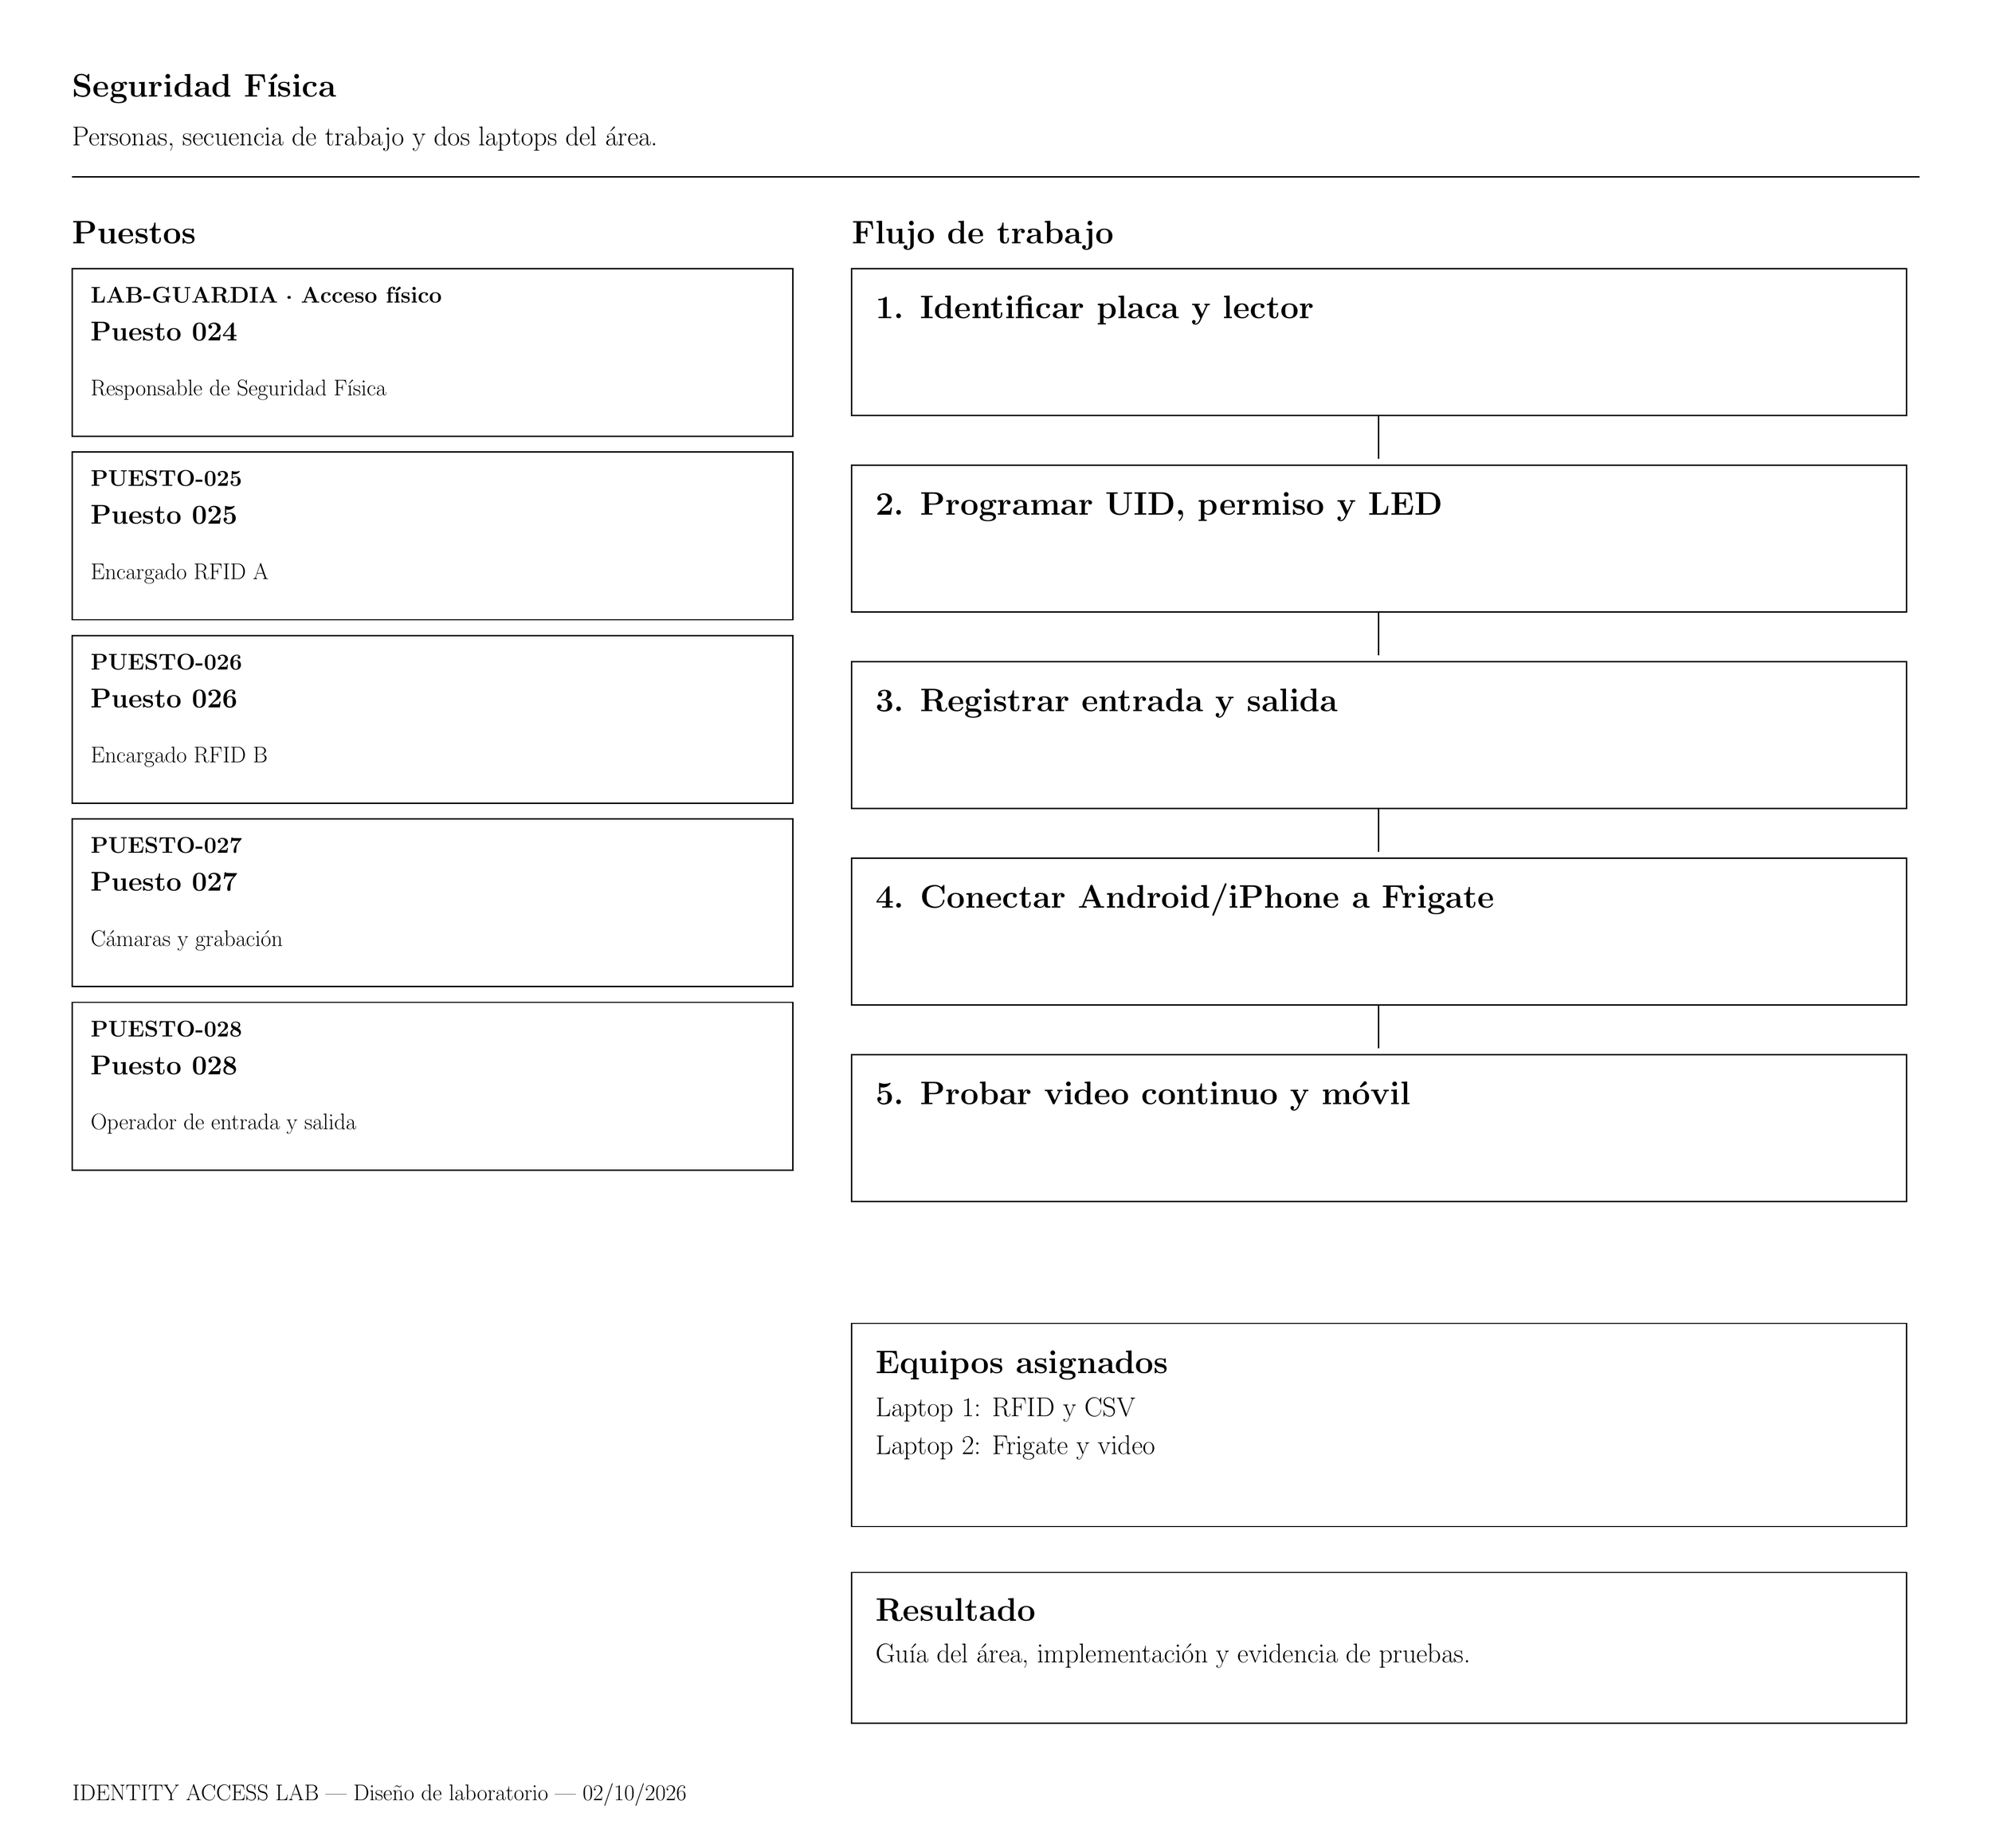
\begin{tikzpicture}[x=1pt,y=-1pt]
\path[use as bounding box] (0,0) rectangle (1500.0,1390.0);
\node[anchor=base west,inner sep=0pt,font=\fontsize{34.0}{40.8}\selectfont \bfseries ] at (45,64) {Seguridad Física};
\node[anchor=base west,inner sep=0pt,font=\fontsize{21.0}{25.2}\selectfont ] at (45,101) {Personas, secuencia de trabajo y dos laptops del área.};
\draw[line width=1pt] (45,125) -- (1455,125);
\node[anchor=base west,inner sep=0pt,font=\fontsize{25.0}{30.0}\selectfont \bfseries ] at (45,176) {Puestos};
\node[anchor=base west,inner sep=0pt,font=\fontsize{25.0}{30.0}\selectfont \bfseries ] at (640,176) {Flujo de trabajo};
\draw[line width=1pt] (45.0,195.0) rectangle (595.0,323.0);
\node[anchor=base west,inner sep=0pt,font=\fontsize{18.0}{21.599999999999998}\selectfont \bfseries ] at (59,221) {LAB-GUARDIA · Acceso físico};
\node[anchor=base west,inner sep=0pt,font=\fontsize{20.0}{24.0}\selectfont \bfseries ] at (59,250) {Puesto 024};
\node[anchor=base west,inner sep=0pt,font=\fontsize{19.0}{22.8}\selectfont ] at (59,292) {Responsable de Seguridad Física};
\draw[line width=1pt] (45.0,335.0) rectangle (595.0,463.0);
\node[anchor=base west,inner sep=0pt,font=\fontsize{18.0}{21.599999999999998}\selectfont \bfseries ] at (59,361) {PUESTO-025};
\node[anchor=base west,inner sep=0pt,font=\fontsize{20.0}{24.0}\selectfont \bfseries ] at (59,390) {Puesto 025};
\node[anchor=base west,inner sep=0pt,font=\fontsize{19.0}{22.8}\selectfont ] at (59,432) {Encargado RFID A};
\draw[line width=1pt] (45.0,475.0) rectangle (595.0,603.0);
\node[anchor=base west,inner sep=0pt,font=\fontsize{18.0}{21.599999999999998}\selectfont \bfseries ] at (59,501) {PUESTO-026};
\node[anchor=base west,inner sep=0pt,font=\fontsize{20.0}{24.0}\selectfont \bfseries ] at (59,530) {Puesto 026};
\node[anchor=base west,inner sep=0pt,font=\fontsize{19.0}{22.8}\selectfont ] at (59,572) {Encargado RFID B};
\draw[line width=1pt] (45.0,615.0) rectangle (595.0,743.0);
\node[anchor=base west,inner sep=0pt,font=\fontsize{18.0}{21.599999999999998}\selectfont \bfseries ] at (59,641) {PUESTO-027};
\node[anchor=base west,inner sep=0pt,font=\fontsize{20.0}{24.0}\selectfont \bfseries ] at (59,670) {Puesto 027};
\node[anchor=base west,inner sep=0pt,font=\fontsize{19.0}{22.8}\selectfont ] at (59,712) {Cámaras y grabación};
\draw[line width=1pt] (45.0,755.0) rectangle (595.0,883.0);
\node[anchor=base west,inner sep=0pt,font=\fontsize{18.0}{21.599999999999998}\selectfont \bfseries ] at (59,781) {PUESTO-028};
\node[anchor=base west,inner sep=0pt,font=\fontsize{20.0}{24.0}\selectfont \bfseries ] at (59,810) {Puesto 028};
\node[anchor=base west,inner sep=0pt,font=\fontsize{19.0}{22.8}\selectfont ] at (59,852) {Operador de entrada y salida};
\draw[line width=1pt] (640.0,195.0) rectangle (1445.0,307.0);
\node[anchor=base west,inner sep=0pt,font=\fontsize{24.0}{28.799999999999997}\selectfont \bfseries ] at (658,233) {1. Identificar placa y lector};
\draw[line width=1pt] (1042,307) -- (1042,340);
\draw[line width=1pt] (640.0,345.0) rectangle (1445.0,457.0);
\node[anchor=base west,inner sep=0pt,font=\fontsize{24.0}{28.799999999999997}\selectfont \bfseries ] at (658,383) {2. Programar UID, permiso y LED};
\draw[line width=1pt] (1042,457) -- (1042,490);
\draw[line width=1pt] (640.0,495.0) rectangle (1445.0,607.0);
\node[anchor=base west,inner sep=0pt,font=\fontsize{24.0}{28.799999999999997}\selectfont \bfseries ] at (658,533) {3. Registrar entrada y salida};
\draw[line width=1pt] (1042,607) -- (1042,640);
\draw[line width=1pt] (640.0,645.0) rectangle (1445.0,757.0);
\node[anchor=base west,inner sep=0pt,font=\fontsize{24.0}{28.799999999999997}\selectfont \bfseries ] at (658,683) {4. Conectar Android/iPhone a Frigate};
\draw[line width=1pt] (1042,757) -- (1042,790);
\draw[line width=1pt] (640.0,795.0) rectangle (1445.0,907.0);
\node[anchor=base west,inner sep=0pt,font=\fontsize{24.0}{28.799999999999997}\selectfont \bfseries ] at (658,833) {5. Probar video continuo y móvil};
\draw[line width=1pt] (640.0,1000.0) rectangle (1445.0,1155.0);
\node[anchor=base west,inner sep=0pt,font=\fontsize{24.0}{28.799999999999997}\selectfont \bfseries ] at (658,1038) {Equipos asignados};
\node[anchor=base west,inner sep=0pt,font=\fontsize{22.0}{26.4}\selectfont ] at (658,1071) {Laptop 1: RFID y CSV};
\node[anchor=base west,inner sep=0pt,font=\fontsize{22.0}{26.4}\selectfont ] at (658,1100) {Laptop 2: Frigate y video};
\draw[line width=1pt] (640.0,1190.0) rectangle (1445.0,1305.0);
\node[anchor=base west,inner sep=0pt,font=\fontsize{23.0}{27.599999999999998}\selectfont \bfseries ] at (658,1227) {Resultado};
\node[anchor=base west,inner sep=0pt,font=\fontsize{21.0}{25.2}\selectfont ] at (658,1259) {Guía del área, implementación y evidencia de pruebas.};
\node[anchor=base west,inner sep=0pt,font=\fontsize{18.0}{21.599999999999998}\selectfont ] at (45,1364) {IDENTITY ACCESS LAB | Diseño de laboratorio | 02/10/2026};
\end{tikzpicture}}
\clearpage
\noindent\resizebox{\textwidth}{!}{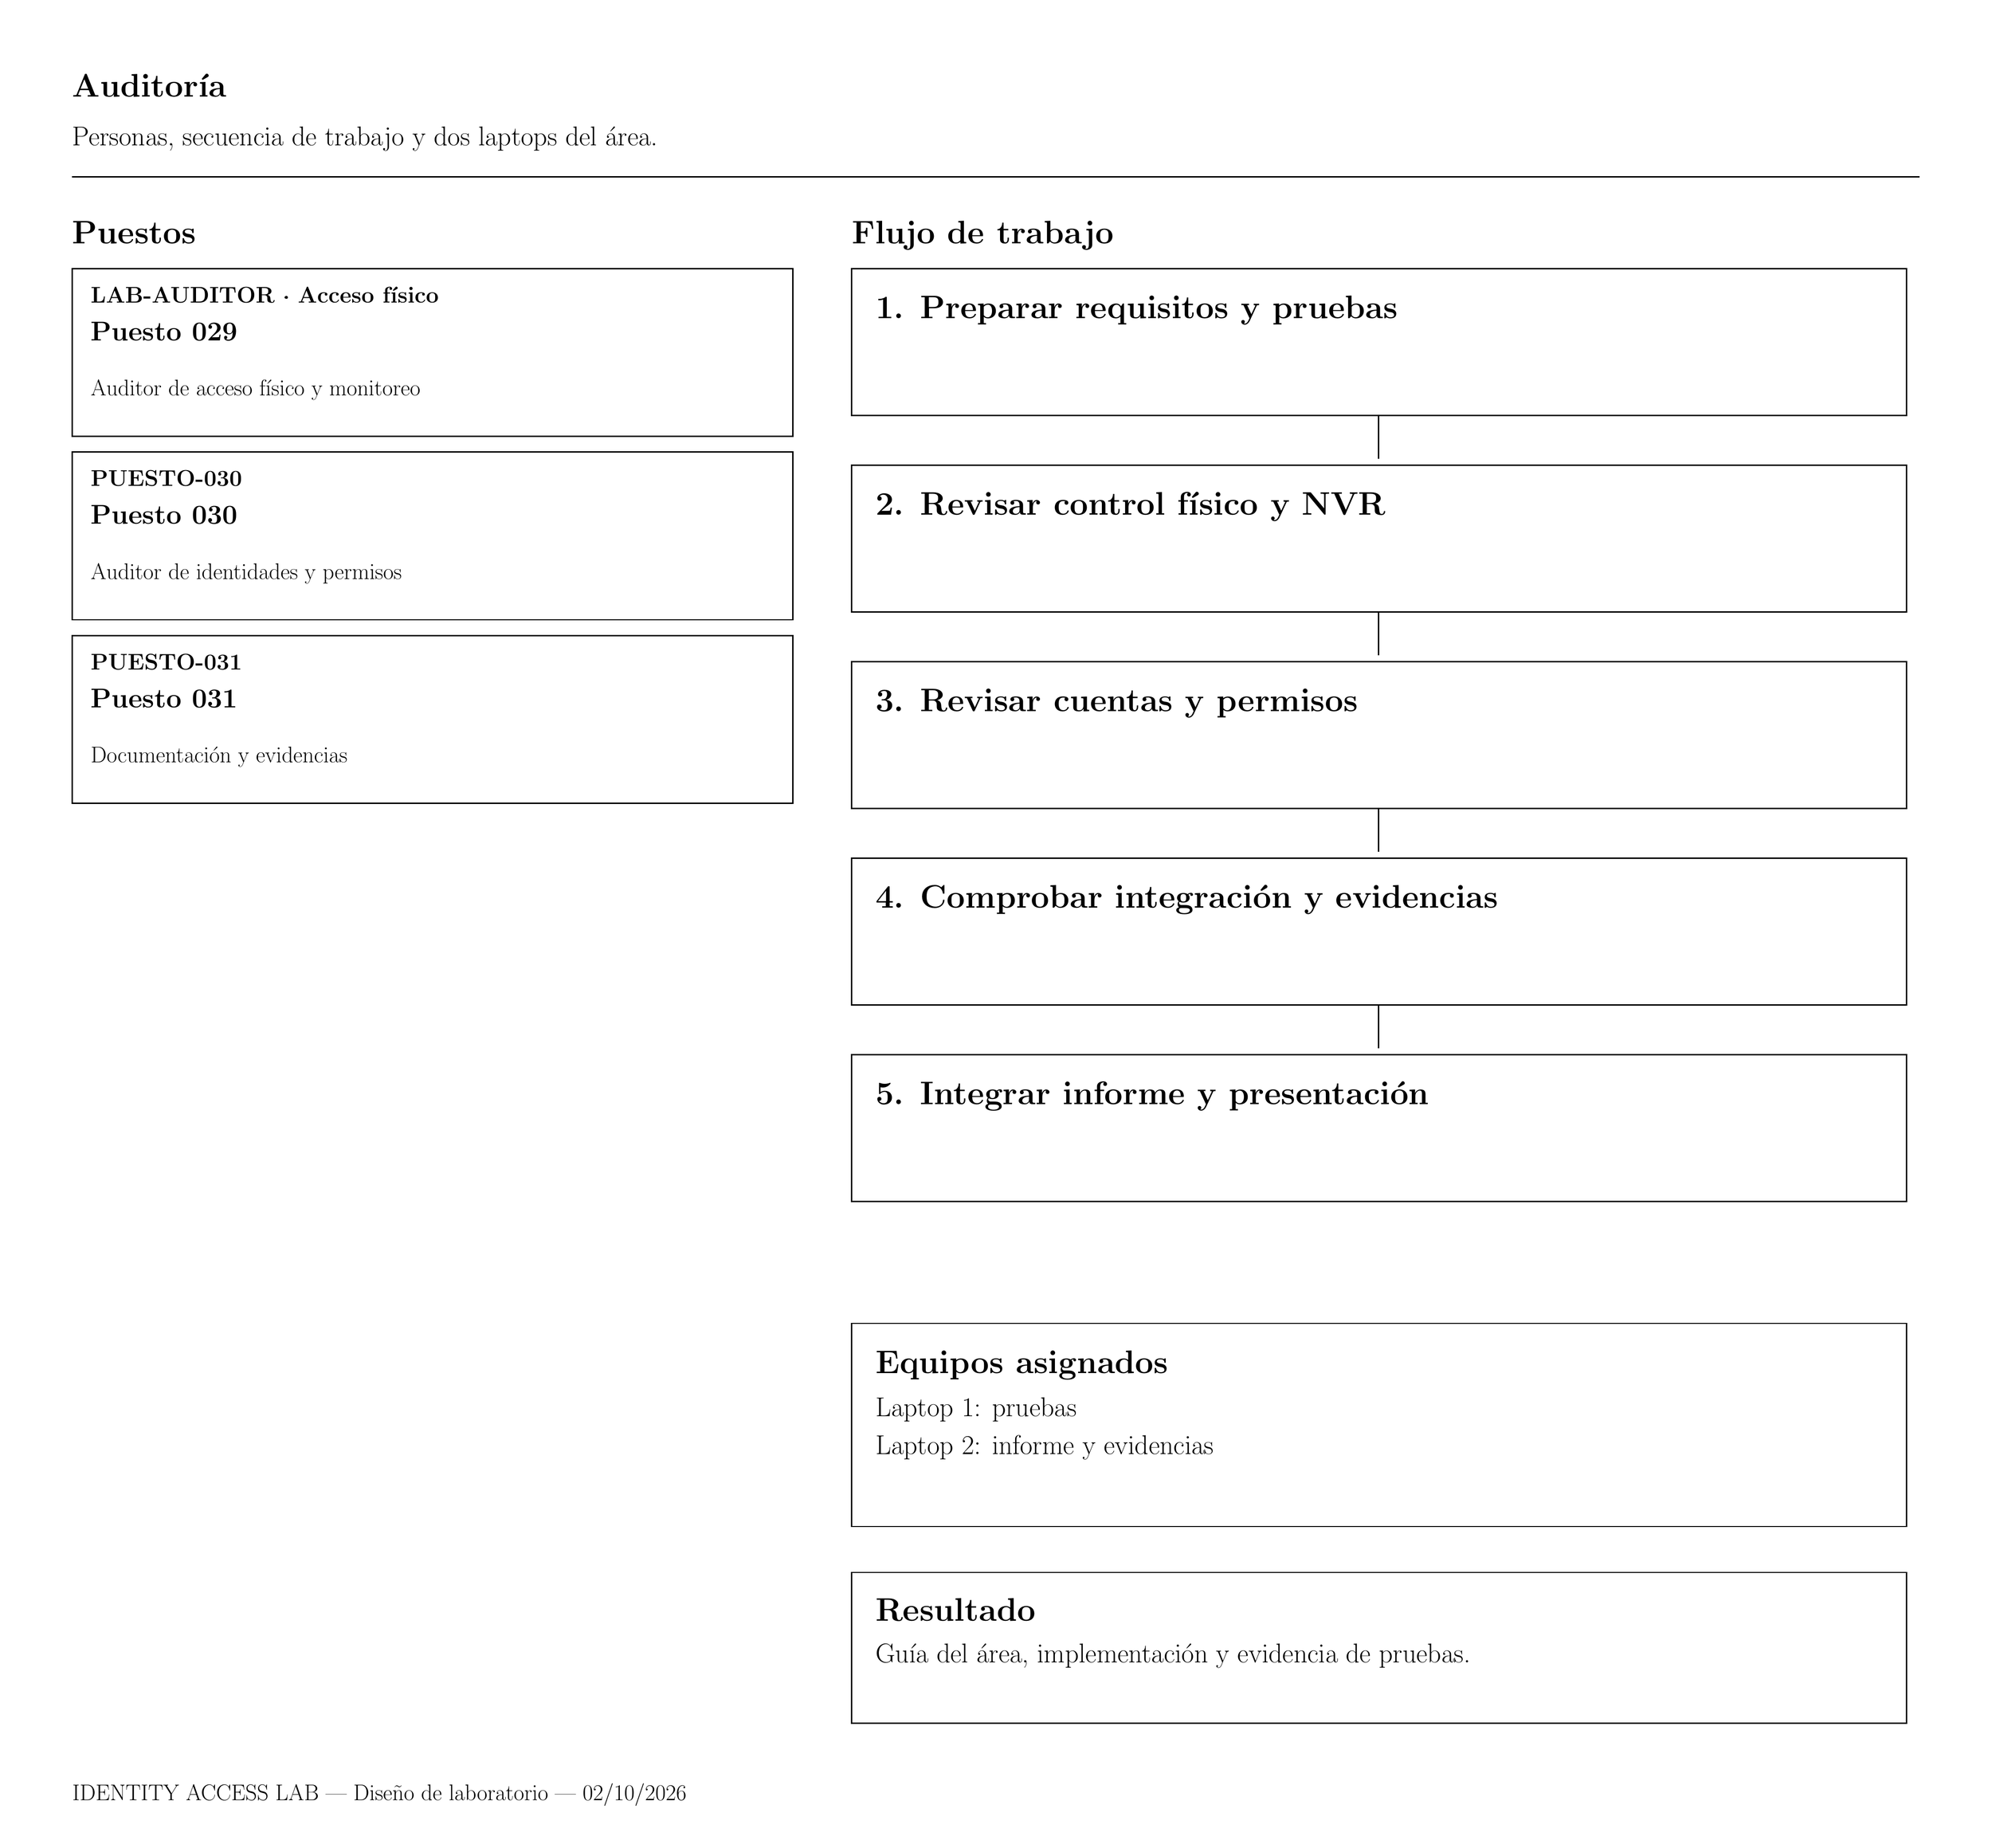
\begin{tikzpicture}[x=1pt,y=-1pt]
\path[use as bounding box] (0,0) rectangle (1500.0,1390.0);
\node[anchor=base west,inner sep=0pt,font=\fontsize{34.0}{40.8}\selectfont \bfseries ] at (45,64) {Auditoría};
\node[anchor=base west,inner sep=0pt,font=\fontsize{21.0}{25.2}\selectfont ] at (45,101) {Personas, secuencia de trabajo y dos laptops del área.};
\draw[line width=1pt] (45,125) -- (1455,125);
\node[anchor=base west,inner sep=0pt,font=\fontsize{25.0}{30.0}\selectfont \bfseries ] at (45,176) {Puestos};
\node[anchor=base west,inner sep=0pt,font=\fontsize{25.0}{30.0}\selectfont \bfseries ] at (640,176) {Flujo de trabajo};
\draw[line width=1pt] (45.0,195.0) rectangle (595.0,323.0);
\node[anchor=base west,inner sep=0pt,font=\fontsize{18.0}{21.599999999999998}\selectfont \bfseries ] at (59,221) {LAB-AUDITOR · Acceso físico};
\node[anchor=base west,inner sep=0pt,font=\fontsize{20.0}{24.0}\selectfont \bfseries ] at (59,250) {Puesto 029};
\node[anchor=base west,inner sep=0pt,font=\fontsize{19.0}{22.8}\selectfont ] at (59,292) {Auditor de acceso físico y monitoreo};
\draw[line width=1pt] (45.0,335.0) rectangle (595.0,463.0);
\node[anchor=base west,inner sep=0pt,font=\fontsize{18.0}{21.599999999999998}\selectfont \bfseries ] at (59,361) {PUESTO-030};
\node[anchor=base west,inner sep=0pt,font=\fontsize{20.0}{24.0}\selectfont \bfseries ] at (59,390) {Puesto 030};
\node[anchor=base west,inner sep=0pt,font=\fontsize{19.0}{22.8}\selectfont ] at (59,432) {Auditor de identidades y permisos};
\draw[line width=1pt] (45.0,475.0) rectangle (595.0,603.0);
\node[anchor=base west,inner sep=0pt,font=\fontsize{18.0}{21.599999999999998}\selectfont \bfseries ] at (59,501) {PUESTO-031};
\node[anchor=base west,inner sep=0pt,font=\fontsize{20.0}{24.0}\selectfont \bfseries ] at (59,530) {Puesto 031};
\node[anchor=base west,inner sep=0pt,font=\fontsize{19.0}{22.8}\selectfont ] at (59,572) {Documentación y evidencias};
\draw[line width=1pt] (640.0,195.0) rectangle (1445.0,307.0);
\node[anchor=base west,inner sep=0pt,font=\fontsize{24.0}{28.799999999999997}\selectfont \bfseries ] at (658,233) {1. Preparar requisitos y pruebas};
\draw[line width=1pt] (1042,307) -- (1042,340);
\draw[line width=1pt] (640.0,345.0) rectangle (1445.0,457.0);
\node[anchor=base west,inner sep=0pt,font=\fontsize{24.0}{28.799999999999997}\selectfont \bfseries ] at (658,383) {2. Revisar control físico y NVR};
\draw[line width=1pt] (1042,457) -- (1042,490);
\draw[line width=1pt] (640.0,495.0) rectangle (1445.0,607.0);
\node[anchor=base west,inner sep=0pt,font=\fontsize{24.0}{28.799999999999997}\selectfont \bfseries ] at (658,533) {3. Revisar cuentas y permisos};
\draw[line width=1pt] (1042,607) -- (1042,640);
\draw[line width=1pt] (640.0,645.0) rectangle (1445.0,757.0);
\node[anchor=base west,inner sep=0pt,font=\fontsize{24.0}{28.799999999999997}\selectfont \bfseries ] at (658,683) {4. Comprobar integración y evidencias};
\draw[line width=1pt] (1042,757) -- (1042,790);
\draw[line width=1pt] (640.0,795.0) rectangle (1445.0,907.0);
\node[anchor=base west,inner sep=0pt,font=\fontsize{24.0}{28.799999999999997}\selectfont \bfseries ] at (658,833) {5. Integrar informe y presentación};
\draw[line width=1pt] (640.0,1000.0) rectangle (1445.0,1155.0);
\node[anchor=base west,inner sep=0pt,font=\fontsize{24.0}{28.799999999999997}\selectfont \bfseries ] at (658,1038) {Equipos asignados};
\node[anchor=base west,inner sep=0pt,font=\fontsize{22.0}{26.4}\selectfont ] at (658,1071) {Laptop 1: pruebas};
\node[anchor=base west,inner sep=0pt,font=\fontsize{22.0}{26.4}\selectfont ] at (658,1100) {Laptop 2: informe y evidencias};
\draw[line width=1pt] (640.0,1190.0) rectangle (1445.0,1305.0);
\node[anchor=base west,inner sep=0pt,font=\fontsize{23.0}{27.599999999999998}\selectfont \bfseries ] at (658,1227) {Resultado};
\node[anchor=base west,inner sep=0pt,font=\fontsize{21.0}{25.2}\selectfont ] at (658,1259) {Guía del área, implementación y evidencia de pruebas.};
\node[anchor=base west,inner sep=0pt,font=\fontsize{18.0}{21.599999999999998}\selectfont ] at (45,1364) {IDENTITY ACCESS LAB | Diseño de laboratorio | 02/10/2026};
\end{tikzpicture}}
\clearpage
\noindent\resizebox{\textwidth}{!}{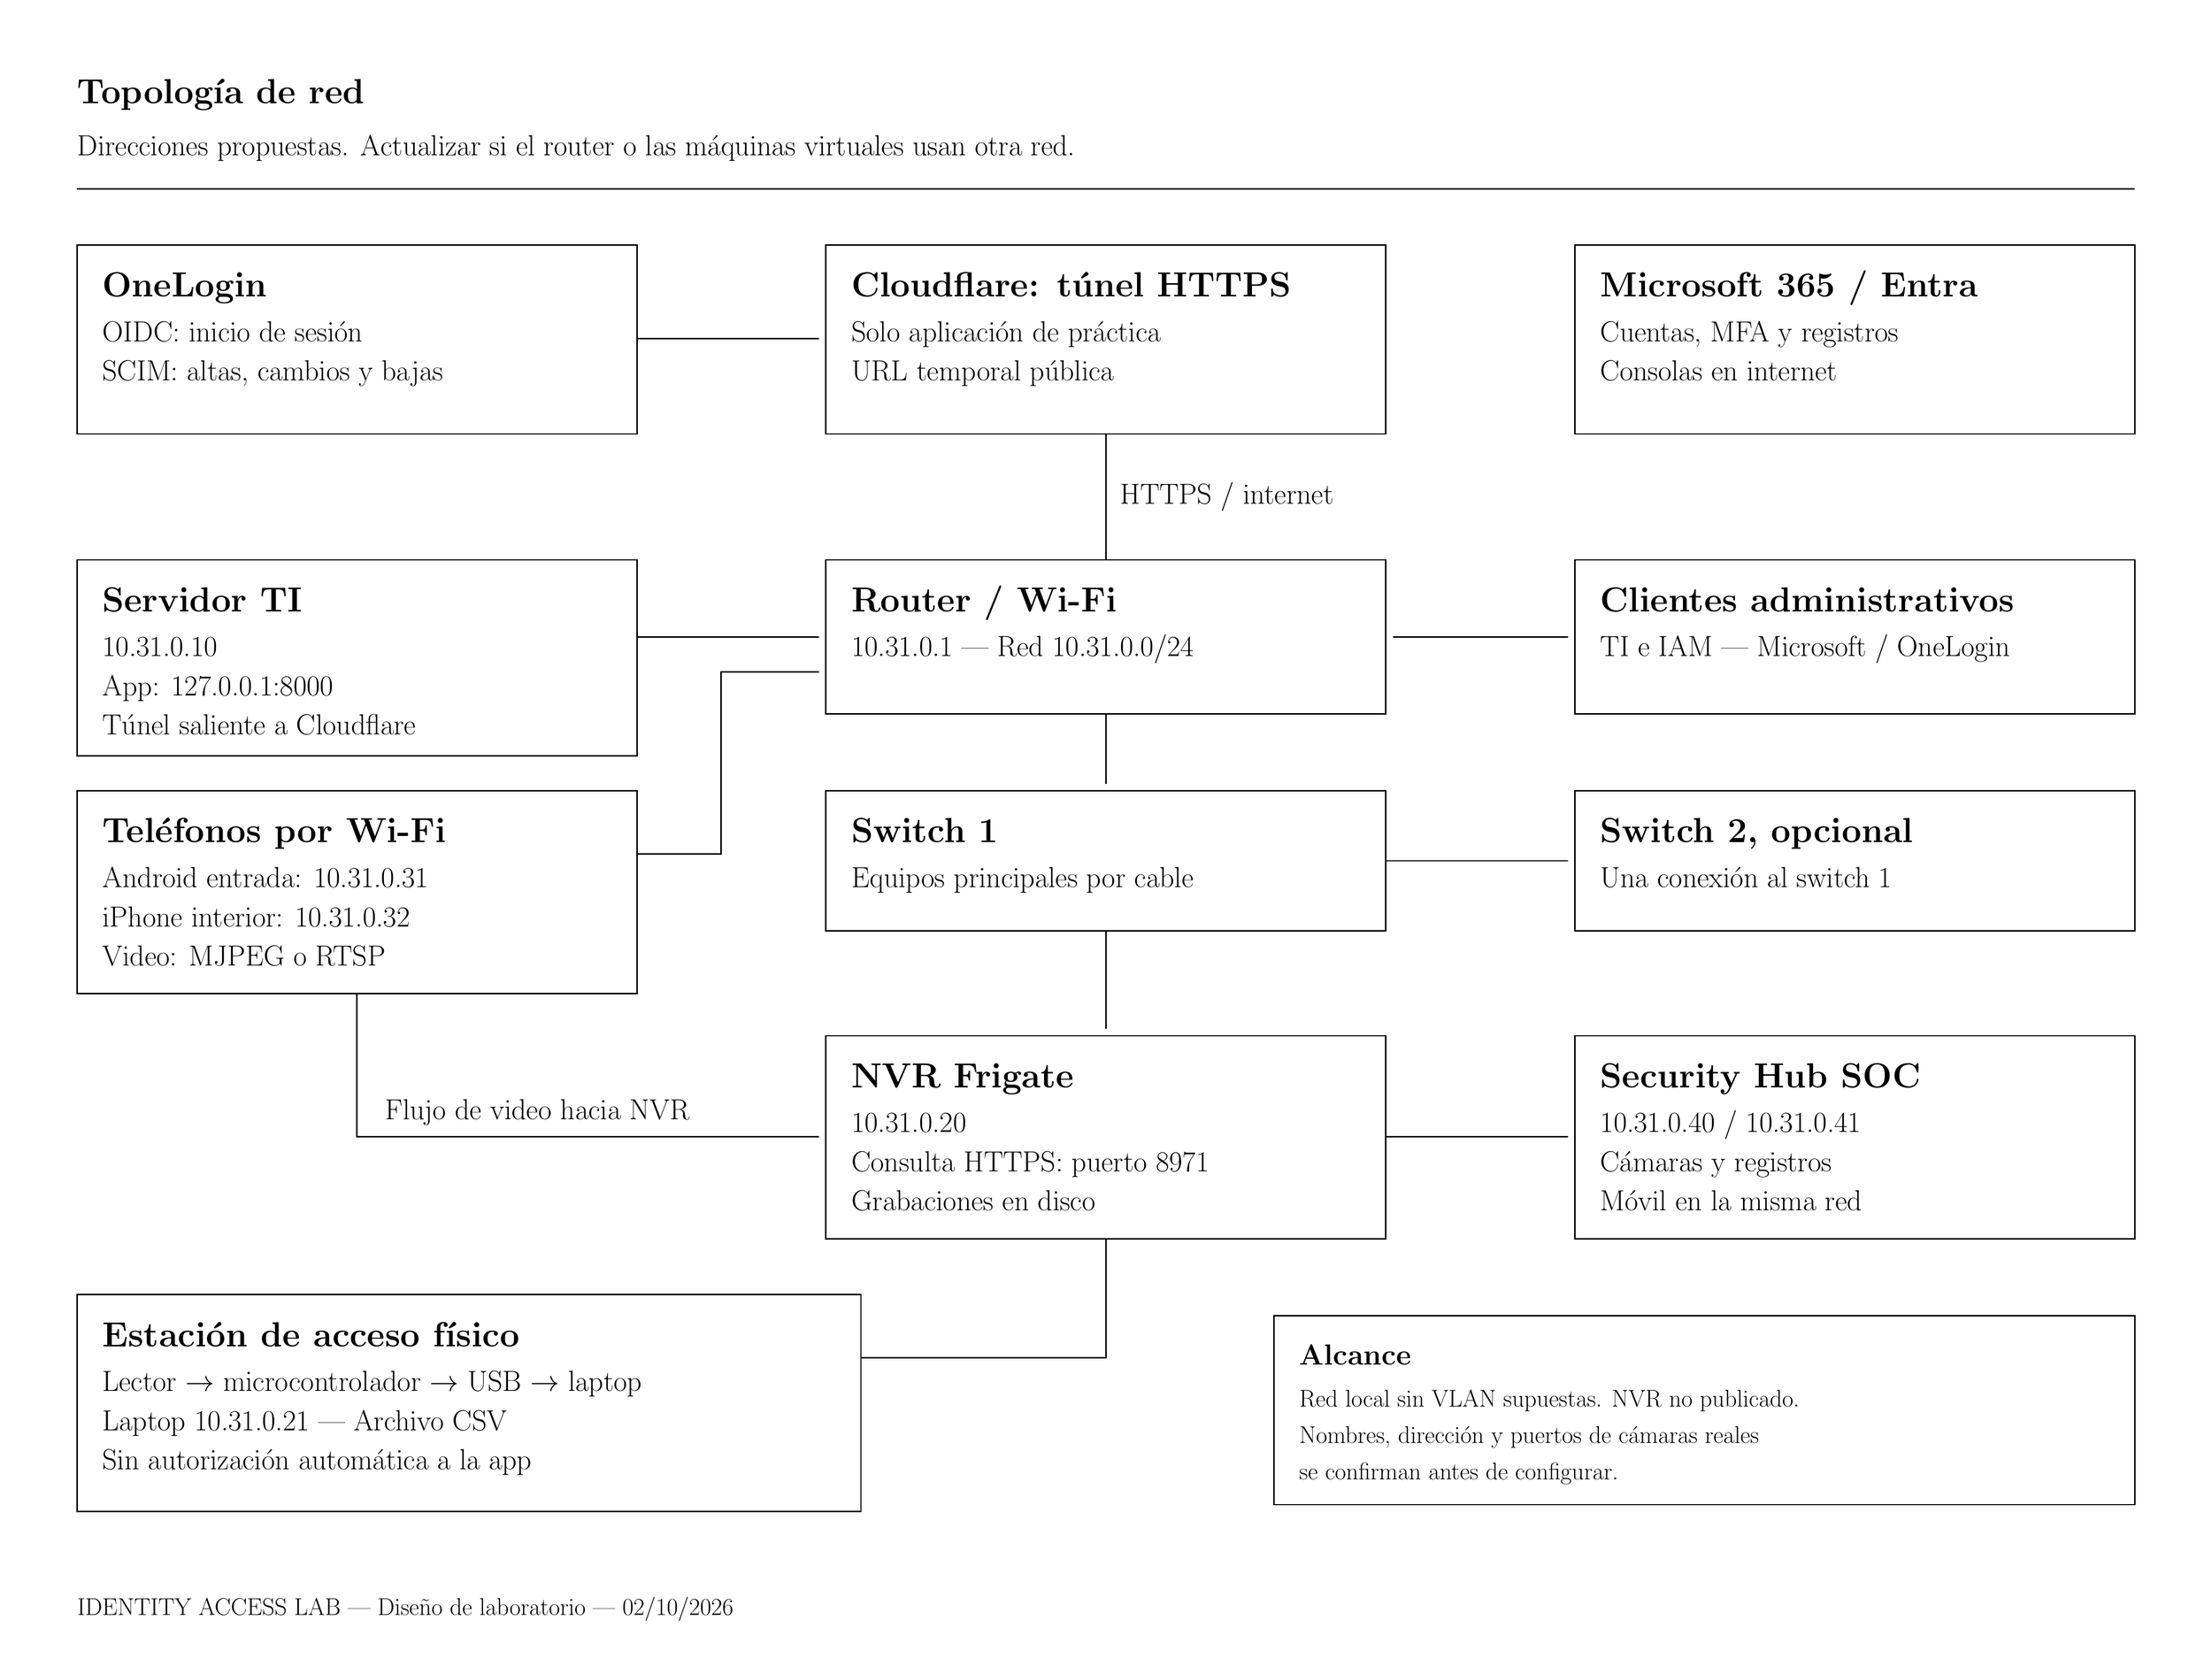
\begin{tikzpicture}[x=1pt,y=-1pt]
\path[use as bounding box] (0,0) rectangle (1560.0,1170.0);
\node[anchor=base west,inner sep=0pt,font=\fontsize{34.0}{40.8}\selectfont \bfseries ] at (45,64) {Topología de red};
\node[anchor=base west,inner sep=0pt,font=\fontsize{21.0}{25.2}\selectfont ] at (45,101) {Direcciones propuestas. Actualizar si el router o las máquinas virtuales usan otra red.};
\draw[line width=1pt] (45,125) -- (1515,125);
\draw[line width=1pt] (45.0,165.0) rectangle (445.0,300.0);
\node[anchor=base west,inner sep=0pt,font=\fontsize{23.0}{27.599999999999998}\selectfont \bfseries ] at (63,202) {OneLogin};
\node[anchor=base west,inner sep=0pt,font=\fontsize{21.0}{25.2}\selectfont ] at (63,234) {OIDC: inicio de sesión};
\node[anchor=base west,inner sep=0pt,font=\fontsize{21.0}{25.2}\selectfont ] at (63,262) {SCIM: altas, cambios y bajas};
\draw[line width=1pt] (580.0,165.0) rectangle (980.0,300.0);
\node[anchor=base west,inner sep=0pt,font=\fontsize{23.0}{27.599999999999998}\selectfont \bfseries ] at (598,202) {Cloudflare: túnel HTTPS};
\node[anchor=base west,inner sep=0pt,font=\fontsize{21.0}{25.2}\selectfont ] at (598,234) {Solo aplicación de práctica};
\node[anchor=base west,inner sep=0pt,font=\fontsize{21.0}{25.2}\selectfont ] at (598,262) {URL temporal pública};
\draw[line width=1pt] (1115.0,165.0) rectangle (1515.0,300.0);
\node[anchor=base west,inner sep=0pt,font=\fontsize{23.0}{27.599999999999998}\selectfont \bfseries ] at (1133,202) {Microsoft 365 / Entra};
\node[anchor=base west,inner sep=0pt,font=\fontsize{21.0}{25.2}\selectfont ] at (1133,234) {Cuentas, MFA y registros};
\node[anchor=base west,inner sep=0pt,font=\fontsize{21.0}{25.2}\selectfont ] at (1133,262) {Consolas en internet};
\draw[line width=1pt] (445,232) -- (575,232);
\draw[line width=1pt] (780,300) -- (780,390);
\node[anchor=base west,inner sep=0pt,font=\fontsize{20.0}{24.0}\selectfont ] at (790,350) {HTTPS / internet};
\draw[line width=1pt] (580.0,390.0) rectangle (980.0,500.0);
\node[anchor=base west,inner sep=0pt,font=\fontsize{23.0}{27.599999999999998}\selectfont \bfseries ] at (598,427) {Router / Wi-Fi};
\node[anchor=base west,inner sep=0pt,font=\fontsize{21.0}{25.2}\selectfont ] at (598,459) {10.31.0.1 | Red 10.31.0.0/24};
\draw[line width=1pt] (45.0,390.0) rectangle (445.0,530.0);
\node[anchor=base west,inner sep=0pt,font=\fontsize{23.0}{27.599999999999998}\selectfont \bfseries ] at (63,427) {Servidor TI};
\node[anchor=base west,inner sep=0pt,font=\fontsize{21.0}{25.2}\selectfont ] at (63,459) {10.31.0.10};
\node[anchor=base west,inner sep=0pt,font=\fontsize{21.0}{25.2}\selectfont ] at (63,487) {App: 127.0.0.1:8000};
\node[anchor=base west,inner sep=0pt,font=\fontsize{21.0}{25.2}\selectfont ] at (63,515) {Túnel saliente a Cloudflare};
\draw[line width=1pt] (445,445) -- (575,445);
\draw[line width=1pt] (1115.0,390.0) rectangle (1515.0,500.0);
\node[anchor=base west,inner sep=0pt,font=\fontsize{23.0}{27.599999999999998}\selectfont \bfseries ] at (1133,427) {Clientes administrativos};
\node[anchor=base west,inner sep=0pt,font=\fontsize{21.0}{25.2}\selectfont ] at (1133,459) {TI e IAM | Microsoft / OneLogin};
\draw[line width=1pt] (985,445) -- (1110,445);
\draw[line width=1pt] (580.0,555.0) rectangle (980.0,655.0);
\node[anchor=base west,inner sep=0pt,font=\fontsize{23.0}{27.599999999999998}\selectfont \bfseries ] at (598,592) {Switch 1};
\node[anchor=base west,inner sep=0pt,font=\fontsize{21.0}{25.2}\selectfont ] at (598,624) {Equipos principales por cable};
\draw[line width=1pt] (780,500) -- (780,550);
\draw[line width=1pt] (45.0,555.0) rectangle (445.0,700.0);
\node[anchor=base west,inner sep=0pt,font=\fontsize{23.0}{27.599999999999998}\selectfont \bfseries ] at (63,592) {Teléfonos por Wi-Fi};
\node[anchor=base west,inner sep=0pt,font=\fontsize{21.0}{25.2}\selectfont ] at (63,624) {Android entrada: 10.31.0.31};
\node[anchor=base west,inner sep=0pt,font=\fontsize{21.0}{25.2}\selectfont ] at (63,652) {iPhone interior: 10.31.0.32};
\node[anchor=base west,inner sep=0pt,font=\fontsize{21.0}{25.2}\selectfont ] at (63,680) {Video: MJPEG o RTSP};
\draw[line width=1pt] (445,600) -- (505,600) -- (505,470) -- (575,470);
\draw[line width=1pt] (1115.0,555.0) rectangle (1515.0,655.0);
\node[anchor=base west,inner sep=0pt,font=\fontsize{23.0}{27.599999999999998}\selectfont \bfseries ] at (1133,592) {Switch 2, opcional};
\node[anchor=base west,inner sep=0pt,font=\fontsize{21.0}{25.2}\selectfont ] at (1133,624) {Una conexión al switch 1};
\draw[line width=1pt] (980,605) -- (1110,605);
\draw[line width=1pt] (580.0,730.0) rectangle (980.0,875.0);
\node[anchor=base west,inner sep=0pt,font=\fontsize{23.0}{27.599999999999998}\selectfont \bfseries ] at (598,767) {NVR Frigate};
\node[anchor=base west,inner sep=0pt,font=\fontsize{21.0}{25.2}\selectfont ] at (598,799) {10.31.0.20};
\node[anchor=base west,inner sep=0pt,font=\fontsize{21.0}{25.2}\selectfont ] at (598,827) {Consulta HTTPS: puerto 8971};
\node[anchor=base west,inner sep=0pt,font=\fontsize{21.0}{25.2}\selectfont ] at (598,855) {Grabaciones en disco};
\draw[line width=1pt] (780,655) -- (780,725);
\draw[line width=1pt] (245,700) -- (245,802) -- (575,802);
\node[anchor=base west,inner sep=0pt,font=\fontsize{20.0}{24.0}\selectfont ] at (265,790) {Flujo de video hacia NVR};
\draw[line width=1pt] (1115.0,730.0) rectangle (1515.0,875.0);
\node[anchor=base west,inner sep=0pt,font=\fontsize{23.0}{27.599999999999998}\selectfont \bfseries ] at (1133,767) {Security Hub SOC};
\node[anchor=base west,inner sep=0pt,font=\fontsize{21.0}{25.2}\selectfont ] at (1133,799) {10.31.0.40 / 10.31.0.41};
\node[anchor=base west,inner sep=0pt,font=\fontsize{21.0}{25.2}\selectfont ] at (1133,827) {Cámaras y registros};
\node[anchor=base west,inner sep=0pt,font=\fontsize{21.0}{25.2}\selectfont ] at (1133,855) {Móvil en la misma red};
\draw[line width=1pt] (980,802) -- (1110,802);
\draw[line width=1pt] (45.0,915.0) rectangle (605.0,1070.0);
\node[anchor=base west,inner sep=0pt,font=\fontsize{23.0}{27.599999999999998}\selectfont \bfseries ] at (63,952) {Estación de acceso físico};
\node[anchor=base west,inner sep=0pt,font=\fontsize{21.0}{25.2}\selectfont ] at (63,984) {Lector \(\rightarrow\) microcontrolador \(\rightarrow\) USB \(\rightarrow\) laptop};
\node[anchor=base west,inner sep=0pt,font=\fontsize{21.0}{25.2}\selectfont ] at (63,1012) {Laptop 10.31.0.21 | Archivo CSV};
\node[anchor=base west,inner sep=0pt,font=\fontsize{21.0}{25.2}\selectfont ] at (63,1040) {Sin autorización automática a la app};
\draw[line width=1pt] (605,960) -- (780,960) -- (780,875);
\draw[line width=1pt] (900.0,930.0) rectangle (1515.0,1065.0);
\node[anchor=base west,inner sep=0pt,font=\fontsize{21.0}{25.2}\selectfont \bfseries ] at (918,965) {Alcance};
\node[anchor=base west,inner sep=0pt,font=\fontsize{19.0}{22.8}\selectfont ] at (918,995) {Red local sin VLAN supuestas. NVR no publicado.};
\node[anchor=base west,inner sep=0pt,font=\fontsize{19.0}{22.8}\selectfont ] at (918,1021) {Nombres, dirección y puertos de cámaras reales};
\node[anchor=base west,inner sep=0pt,font=\fontsize{19.0}{22.8}\selectfont ] at (918,1047) {se confirman antes de configurar.};
\node[anchor=base west,inner sep=0pt,font=\fontsize{18.0}{21.599999999999998}\selectfont ] at (45,1144) {IDENTITY ACCESS LAB | Diseño de laboratorio | 02/10/2026};
\end{tikzpicture}}
\clearpage
\noindent\resizebox{\textwidth}{!}{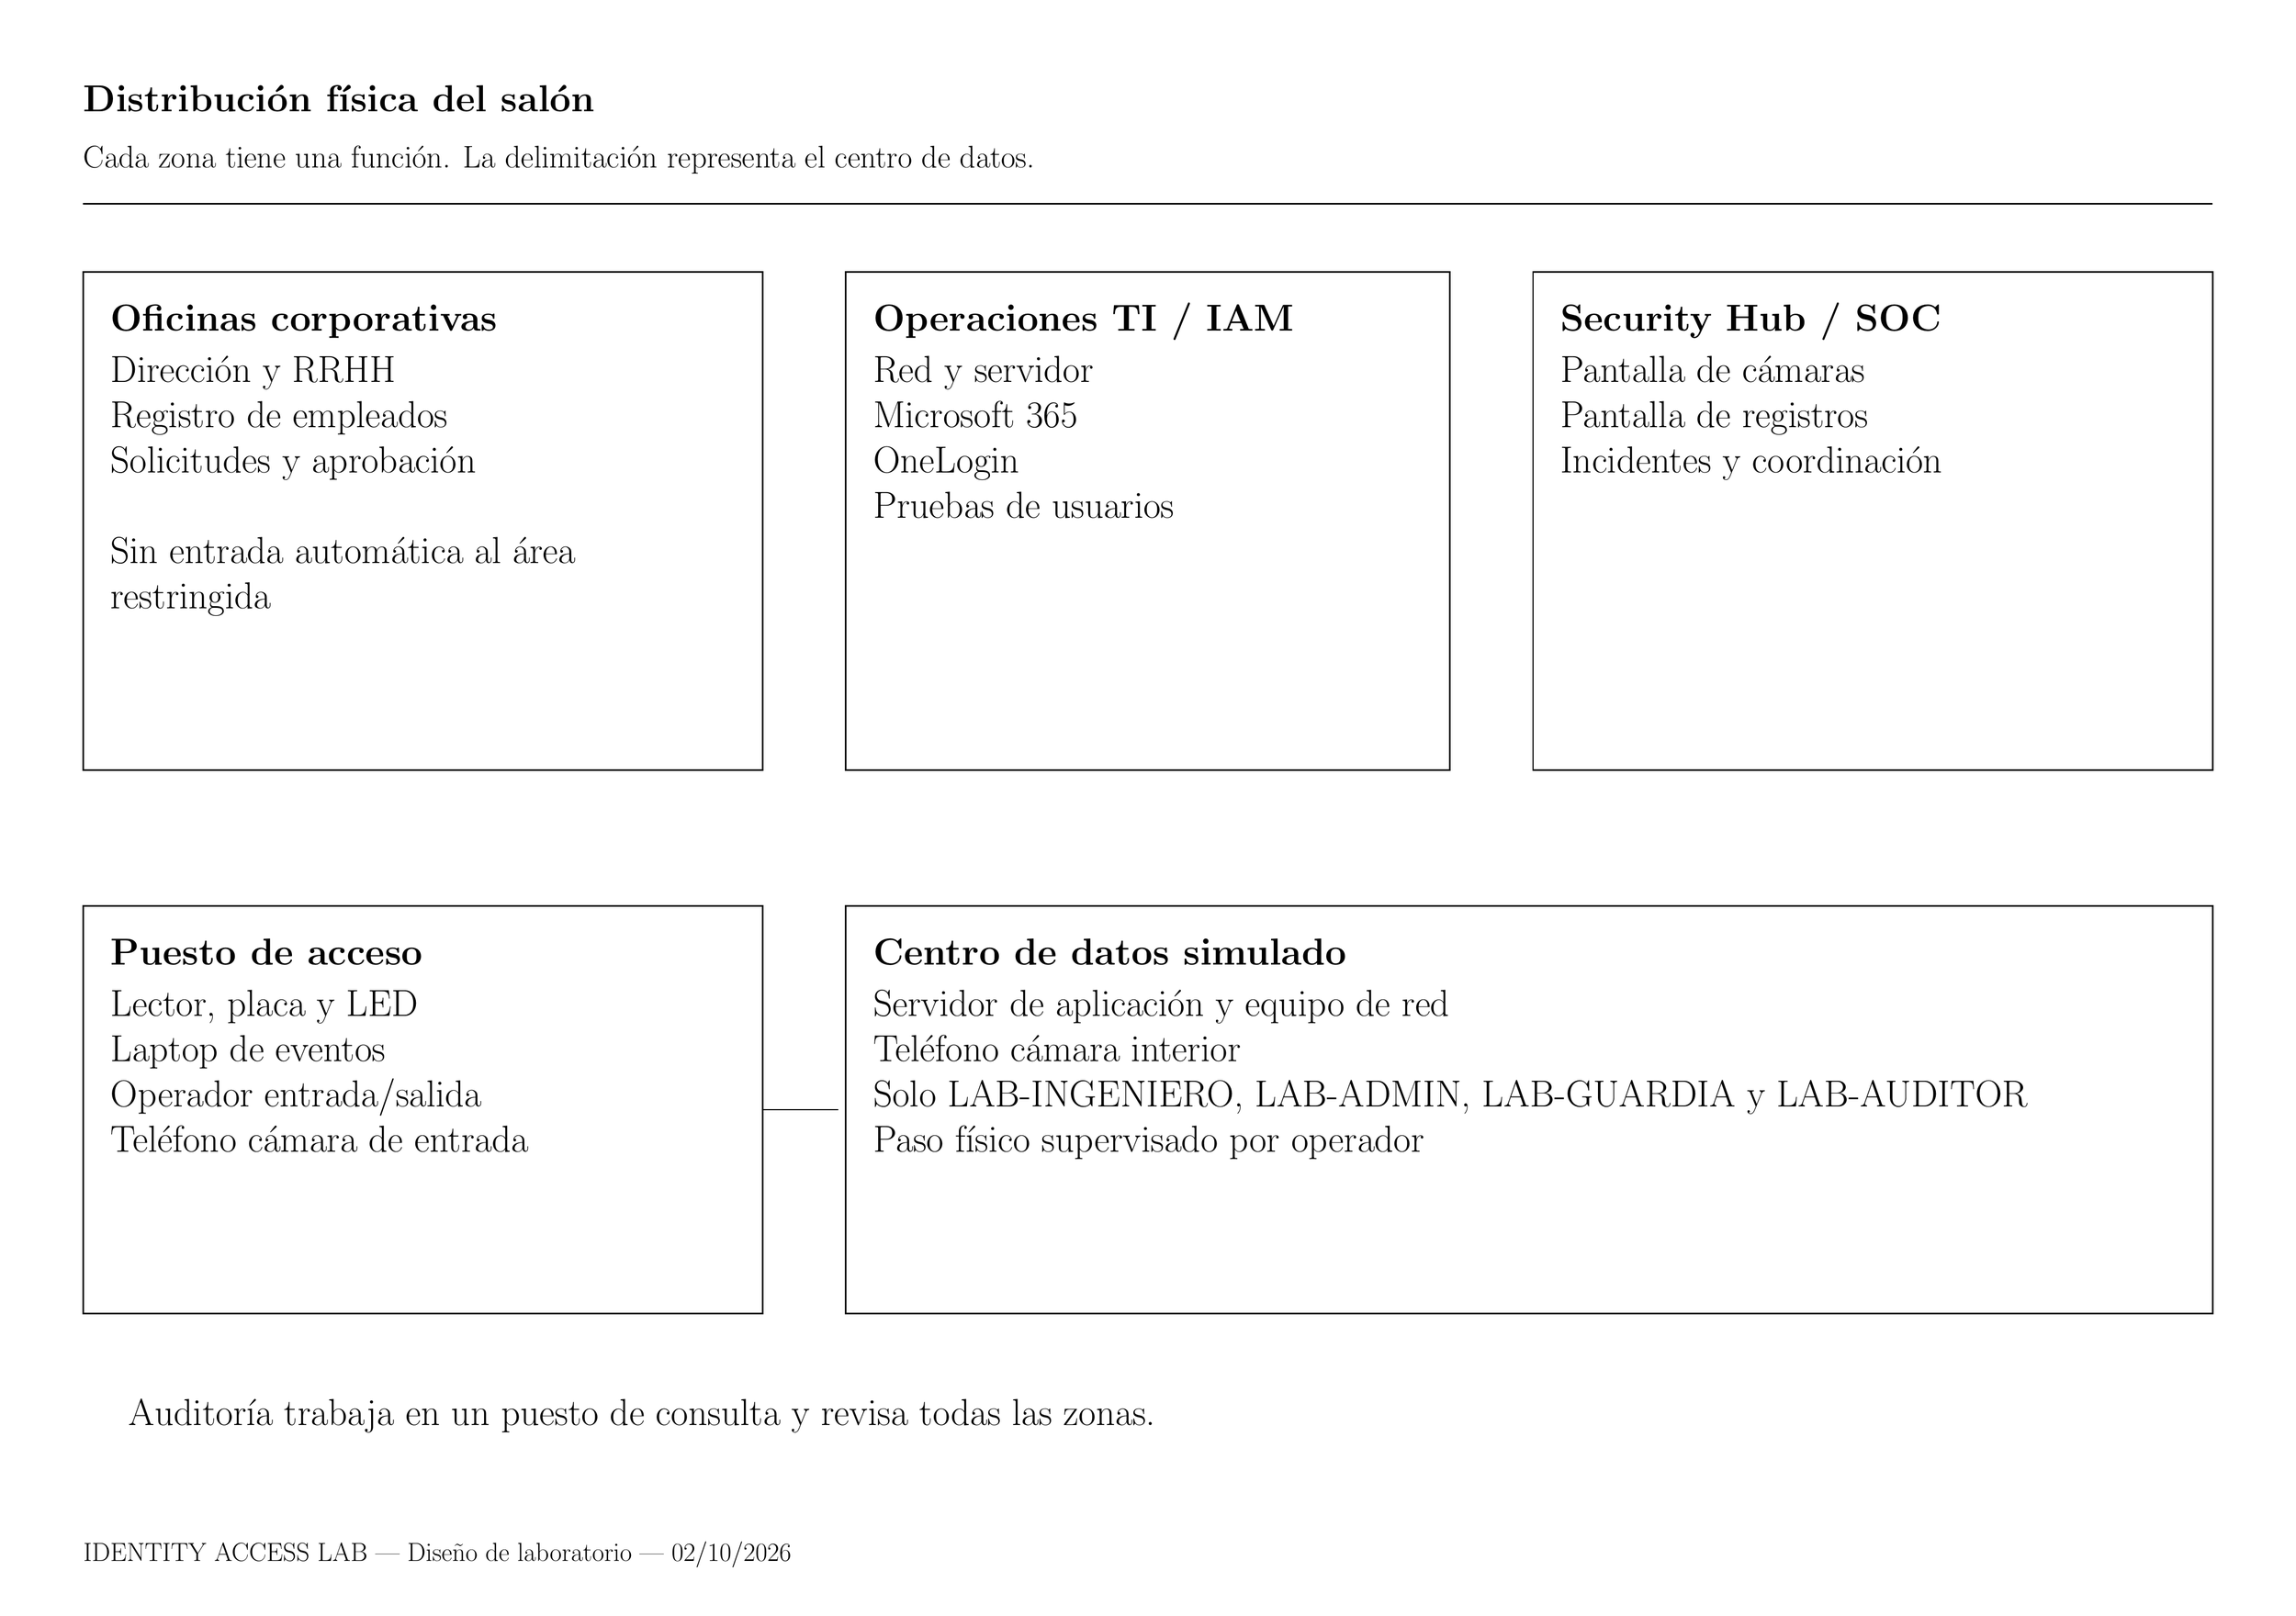
\begin{tikzpicture}[x=1pt,y=-1pt]
\path[use as bounding box] (0,0) rectangle (1500.0,1050.0);
\node[anchor=base west,inner sep=0pt,font=\fontsize{34.0}{40.8}\selectfont \bfseries ] at (45,64) {Distribución física del salón};
\node[anchor=base west,inner sep=0pt,font=\fontsize{21.0}{25.2}\selectfont ] at (45,101) {Cada zona tiene una función. La delimitación representa el centro de datos.};
\draw[line width=1pt] (45,125) -- (1455,125);
\draw[line width=1pt] (45.0,170.0) rectangle (495.0,500.0);
\node[anchor=base west,inner sep=0pt,font=\fontsize{25.0}{30.0}\selectfont \bfseries ] at (63,209) {Oficinas corporativas};
\node[anchor=base west,inner sep=0pt,font=\fontsize{23.0}{27.599999999999998}\selectfont ] at (63,243) {Dirección y RRHH};
\node[anchor=base west,inner sep=0pt,font=\fontsize{23.0}{27.599999999999998}\selectfont ] at (63,273) {Registro de empleados};
\node[anchor=base west,inner sep=0pt,font=\fontsize{23.0}{27.599999999999998}\selectfont ] at (63,303) {Solicitudes y aprobación};
\node[anchor=base west,inner sep=0pt,font=\fontsize{23.0}{27.599999999999998}\selectfont ] at (63,333) {};
\node[anchor=base west,inner sep=0pt,font=\fontsize{23.0}{27.599999999999998}\selectfont ] at (63,363) {Sin entrada automática al área};
\node[anchor=base west,inner sep=0pt,font=\fontsize{23.0}{27.599999999999998}\selectfont ] at (63,393) {restringida};
\draw[line width=1pt] (550.0,170.0) rectangle (950.0,500.0);
\node[anchor=base west,inner sep=0pt,font=\fontsize{25.0}{30.0}\selectfont \bfseries ] at (568,209) {Operaciones TI / IAM};
\node[anchor=base west,inner sep=0pt,font=\fontsize{23.0}{27.599999999999998}\selectfont ] at (568,243) {Red y servidor};
\node[anchor=base west,inner sep=0pt,font=\fontsize{23.0}{27.599999999999998}\selectfont ] at (568,273) {Microsoft 365};
\node[anchor=base west,inner sep=0pt,font=\fontsize{23.0}{27.599999999999998}\selectfont ] at (568,303) {OneLogin};
\node[anchor=base west,inner sep=0pt,font=\fontsize{23.0}{27.599999999999998}\selectfont ] at (568,333) {Pruebas de usuarios};
\draw[line width=1pt] (1005.0,170.0) rectangle (1455.0,500.0);
\node[anchor=base west,inner sep=0pt,font=\fontsize{25.0}{30.0}\selectfont \bfseries ] at (1023,209) {Security Hub / SOC};
\node[anchor=base west,inner sep=0pt,font=\fontsize{23.0}{27.599999999999998}\selectfont ] at (1023,243) {Pantalla de cámaras};
\node[anchor=base west,inner sep=0pt,font=\fontsize{23.0}{27.599999999999998}\selectfont ] at (1023,273) {Pantalla de registros};
\node[anchor=base west,inner sep=0pt,font=\fontsize{23.0}{27.599999999999998}\selectfont ] at (1023,303) {Incidentes y coordinación};
\draw[line width=1pt] (45.0,590.0) rectangle (495.0,860.0);
\node[anchor=base west,inner sep=0pt,font=\fontsize{25.0}{30.0}\selectfont \bfseries ] at (63,629) {Puesto de acceso};
\node[anchor=base west,inner sep=0pt,font=\fontsize{23.0}{27.599999999999998}\selectfont ] at (63,663) {Lector, placa y LED};
\node[anchor=base west,inner sep=0pt,font=\fontsize{23.0}{27.599999999999998}\selectfont ] at (63,693) {Laptop de eventos};
\node[anchor=base west,inner sep=0pt,font=\fontsize{23.0}{27.599999999999998}\selectfont ] at (63,723) {Operador entrada/salida};
\node[anchor=base west,inner sep=0pt,font=\fontsize{23.0}{27.599999999999998}\selectfont ] at (63,753) {Teléfono cámara de entrada};
\draw[line width=1pt] (550.0,590.0) rectangle (1455.0,860.0);
\node[anchor=base west,inner sep=0pt,font=\fontsize{25.0}{30.0}\selectfont \bfseries ] at (568,629) {Centro de datos simulado};
\node[anchor=base west,inner sep=0pt,font=\fontsize{23.0}{27.599999999999998}\selectfont ] at (568,663) {Servidor de aplicación y equipo de red};
\node[anchor=base west,inner sep=0pt,font=\fontsize{23.0}{27.599999999999998}\selectfont ] at (568,693) {Teléfono cámara interior};
\node[anchor=base west,inner sep=0pt,font=\fontsize{23.0}{27.599999999999998}\selectfont ] at (568,723) {Solo LAB-INGENIERO, LAB-ADMIN, LAB-GUARDIA y LAB-AUDITOR};
\node[anchor=base west,inner sep=0pt,font=\fontsize{23.0}{27.599999999999998}\selectfont ] at (568,753) {Paso físico supervisado por operador};
\draw[line width=1pt] (495,725) -- (545,725);
\node[anchor=base west,inner sep=0pt,font=\fontsize{24.0}{28.799999999999997}\selectfont ] at (75,934) {Auditoría trabaja en un puesto de consulta y revisa todas las zonas.};
\node[anchor=base west,inner sep=0pt,font=\fontsize{18.0}{21.599999999999998}\selectfont ] at (45,1024) {IDENTITY ACCESS LAB | Diseño de laboratorio | 02/10/2026};
\end{tikzpicture}}
\clearpage
\noindent\resizebox{\textwidth}{!}{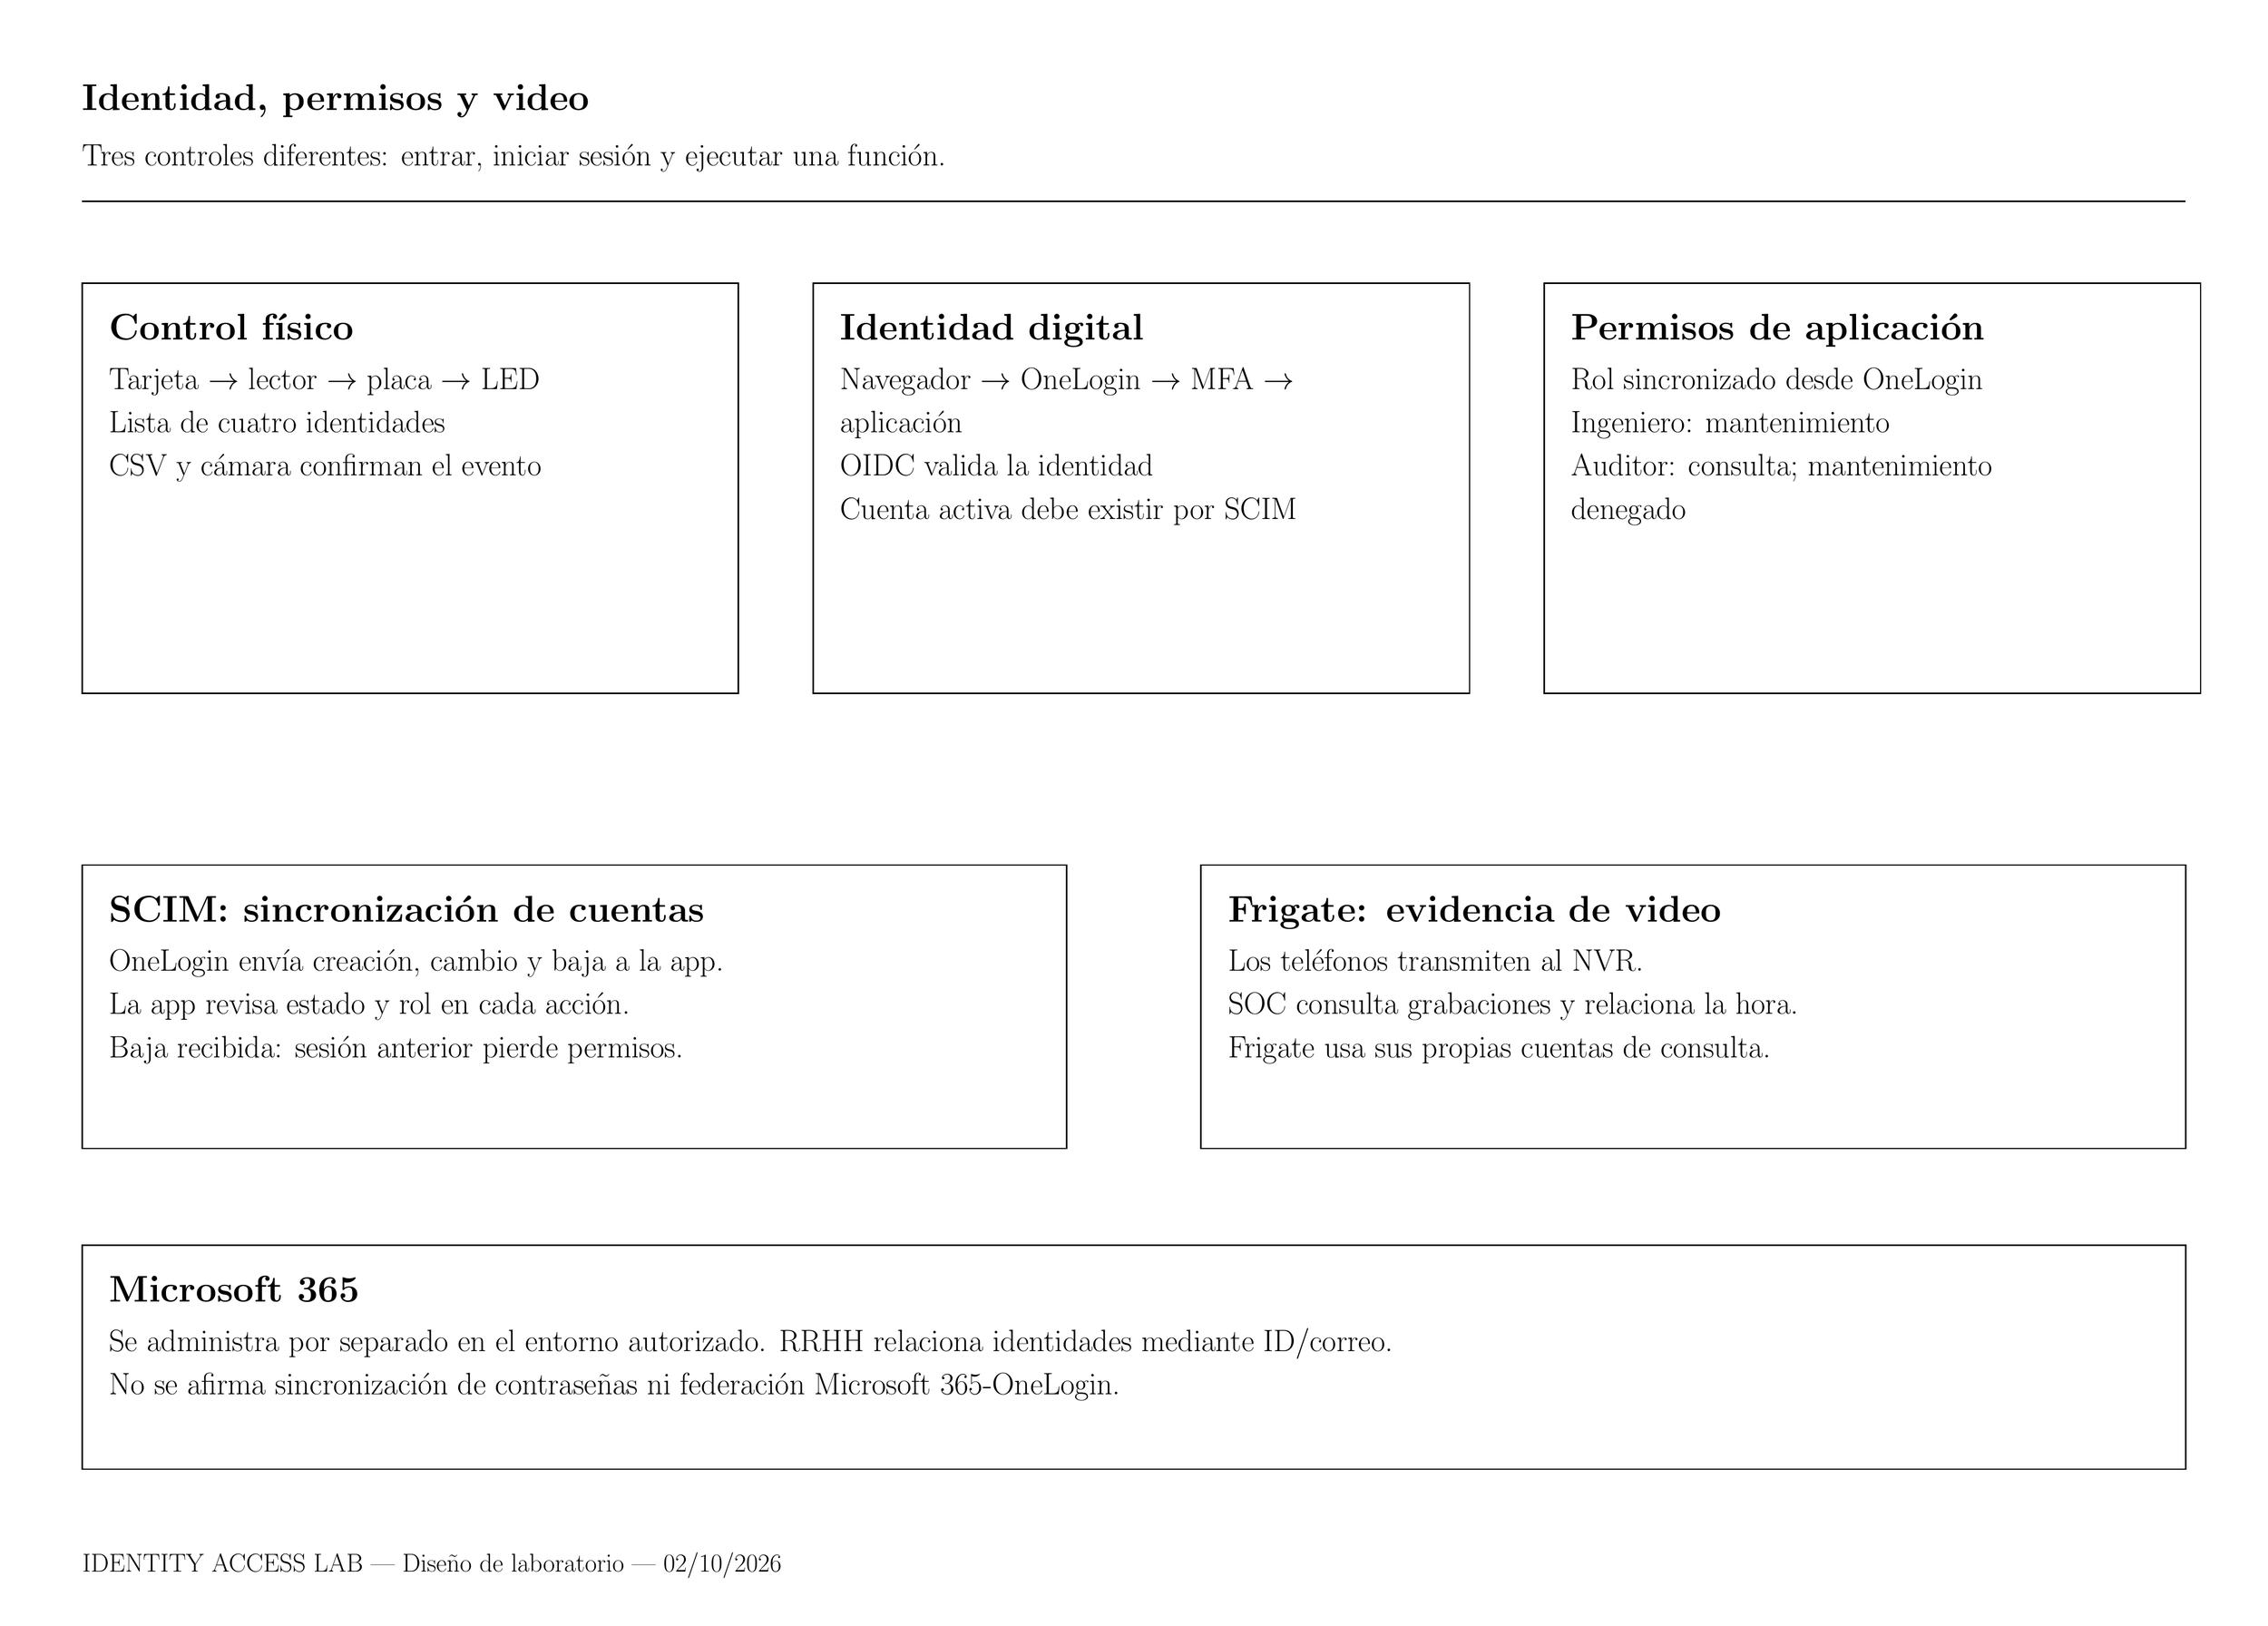
\begin{tikzpicture}[x=1pt,y=-1pt]
\path[use as bounding box] (0,0) rectangle (1500.0,1070.0);
\node[anchor=base west,inner sep=0pt,font=\fontsize{34.0}{40.8}\selectfont \bfseries ] at (45,64) {Identidad, permisos y video};
\node[anchor=base west,inner sep=0pt,font=\fontsize{21.0}{25.2}\selectfont ] at (45,101) {Tres controles diferentes: entrar, iniciar sesión y ejecutar una función.};
\draw[line width=1pt] (45,125) -- (1455,125);
\draw[line width=1pt] (45.0,180.0) rectangle (485.0,455.0);
\node[anchor=base west,inner sep=0pt,font=\fontsize{24.0}{28.799999999999997}\selectfont \bfseries ] at (63,218) {Control físico};
\node[anchor=base west,inner sep=0pt,font=\fontsize{22.0}{26.4}\selectfont ] at (63,251) {Tarjeta \(\rightarrow\) lector \(\rightarrow\) placa \(\rightarrow\) LED};
\node[anchor=base west,inner sep=0pt,font=\fontsize{22.0}{26.4}\selectfont ] at (63,280) {Lista de cuatro identidades};
\node[anchor=base west,inner sep=0pt,font=\fontsize{22.0}{26.4}\selectfont ] at (63,309) {CSV y cámara confirman el evento};
\draw[line width=1pt] (535.0,180.0) rectangle (975.0,455.0);
\node[anchor=base west,inner sep=0pt,font=\fontsize{24.0}{28.799999999999997}\selectfont \bfseries ] at (553,218) {Identidad digital};
\node[anchor=base west,inner sep=0pt,font=\fontsize{22.0}{26.4}\selectfont ] at (553,251) {Navegador \(\rightarrow\) OneLogin \(\rightarrow\) MFA \(\rightarrow\)};
\node[anchor=base west,inner sep=0pt,font=\fontsize{22.0}{26.4}\selectfont ] at (553,280) {aplicación};
\node[anchor=base west,inner sep=0pt,font=\fontsize{22.0}{26.4}\selectfont ] at (553,309) {OIDC valida la identidad};
\node[anchor=base west,inner sep=0pt,font=\fontsize{22.0}{26.4}\selectfont ] at (553,338) {Cuenta activa debe existir por SCIM};
\draw[line width=1pt] (1025.0,180.0) rectangle (1465.0,455.0);
\node[anchor=base west,inner sep=0pt,font=\fontsize{24.0}{28.799999999999997}\selectfont \bfseries ] at (1043,218) {Permisos de aplicación};
\node[anchor=base west,inner sep=0pt,font=\fontsize{22.0}{26.4}\selectfont ] at (1043,251) {Rol sincronizado desde OneLogin};
\node[anchor=base west,inner sep=0pt,font=\fontsize{22.0}{26.4}\selectfont ] at (1043,280) {Ingeniero: mantenimiento};
\node[anchor=base west,inner sep=0pt,font=\fontsize{22.0}{26.4}\selectfont ] at (1043,309) {Auditor: consulta; mantenimiento};
\node[anchor=base west,inner sep=0pt,font=\fontsize{22.0}{26.4}\selectfont ] at (1043,338) {denegado};
\draw[line width=1pt] (45.0,570.0) rectangle (705.0,760.0);
\node[anchor=base west,inner sep=0pt,font=\fontsize{24.0}{28.799999999999997}\selectfont \bfseries ] at (63,608) {SCIM: sincronización de cuentas};
\node[anchor=base west,inner sep=0pt,font=\fontsize{22.0}{26.4}\selectfont ] at (63,641) {OneLogin envía creación, cambio y baja a la app.};
\node[anchor=base west,inner sep=0pt,font=\fontsize{22.0}{26.4}\selectfont ] at (63,670) {La app revisa estado y rol en cada acción.};
\node[anchor=base west,inner sep=0pt,font=\fontsize{22.0}{26.4}\selectfont ] at (63,699) {Baja recibida: sesión anterior pierde permisos.};
\draw[line width=1pt] (795.0,570.0) rectangle (1455.0,760.0);
\node[anchor=base west,inner sep=0pt,font=\fontsize{24.0}{28.799999999999997}\selectfont \bfseries ] at (813,608) {Frigate: evidencia de video};
\node[anchor=base west,inner sep=0pt,font=\fontsize{22.0}{26.4}\selectfont ] at (813,641) {Los teléfonos transmiten al NVR.};
\node[anchor=base west,inner sep=0pt,font=\fontsize{22.0}{26.4}\selectfont ] at (813,670) {SOC consulta grabaciones y relaciona la hora.};
\node[anchor=base west,inner sep=0pt,font=\fontsize{22.0}{26.4}\selectfont ] at (813,699) {Frigate usa sus propias cuentas de consulta.};
\draw[line width=1pt] (45.0,825.0) rectangle (1455.0,975.0);
\node[anchor=base west,inner sep=0pt,font=\fontsize{24.0}{28.799999999999997}\selectfont \bfseries ] at (63,863) {Microsoft 365};
\node[anchor=base west,inner sep=0pt,font=\fontsize{22.0}{26.4}\selectfont ] at (63,896) {Se administra por separado en el entorno autorizado. RRHH relaciona identidades mediante ID/correo.};
\node[anchor=base west,inner sep=0pt,font=\fontsize{22.0}{26.4}\selectfont ] at (63,925) {No se afirma sincronización de contraseñas ni federación Microsoft 365-OneLogin.};
\node[anchor=base west,inner sep=0pt,font=\fontsize{18.0}{21.599999999999998}\selectfont ] at (45,1044) {IDENTITY ACCESS LAB | Diseño de laboratorio | 02/10/2026};
\end{tikzpicture}}
\clearpage
\noindent\resizebox{\textwidth}{!}{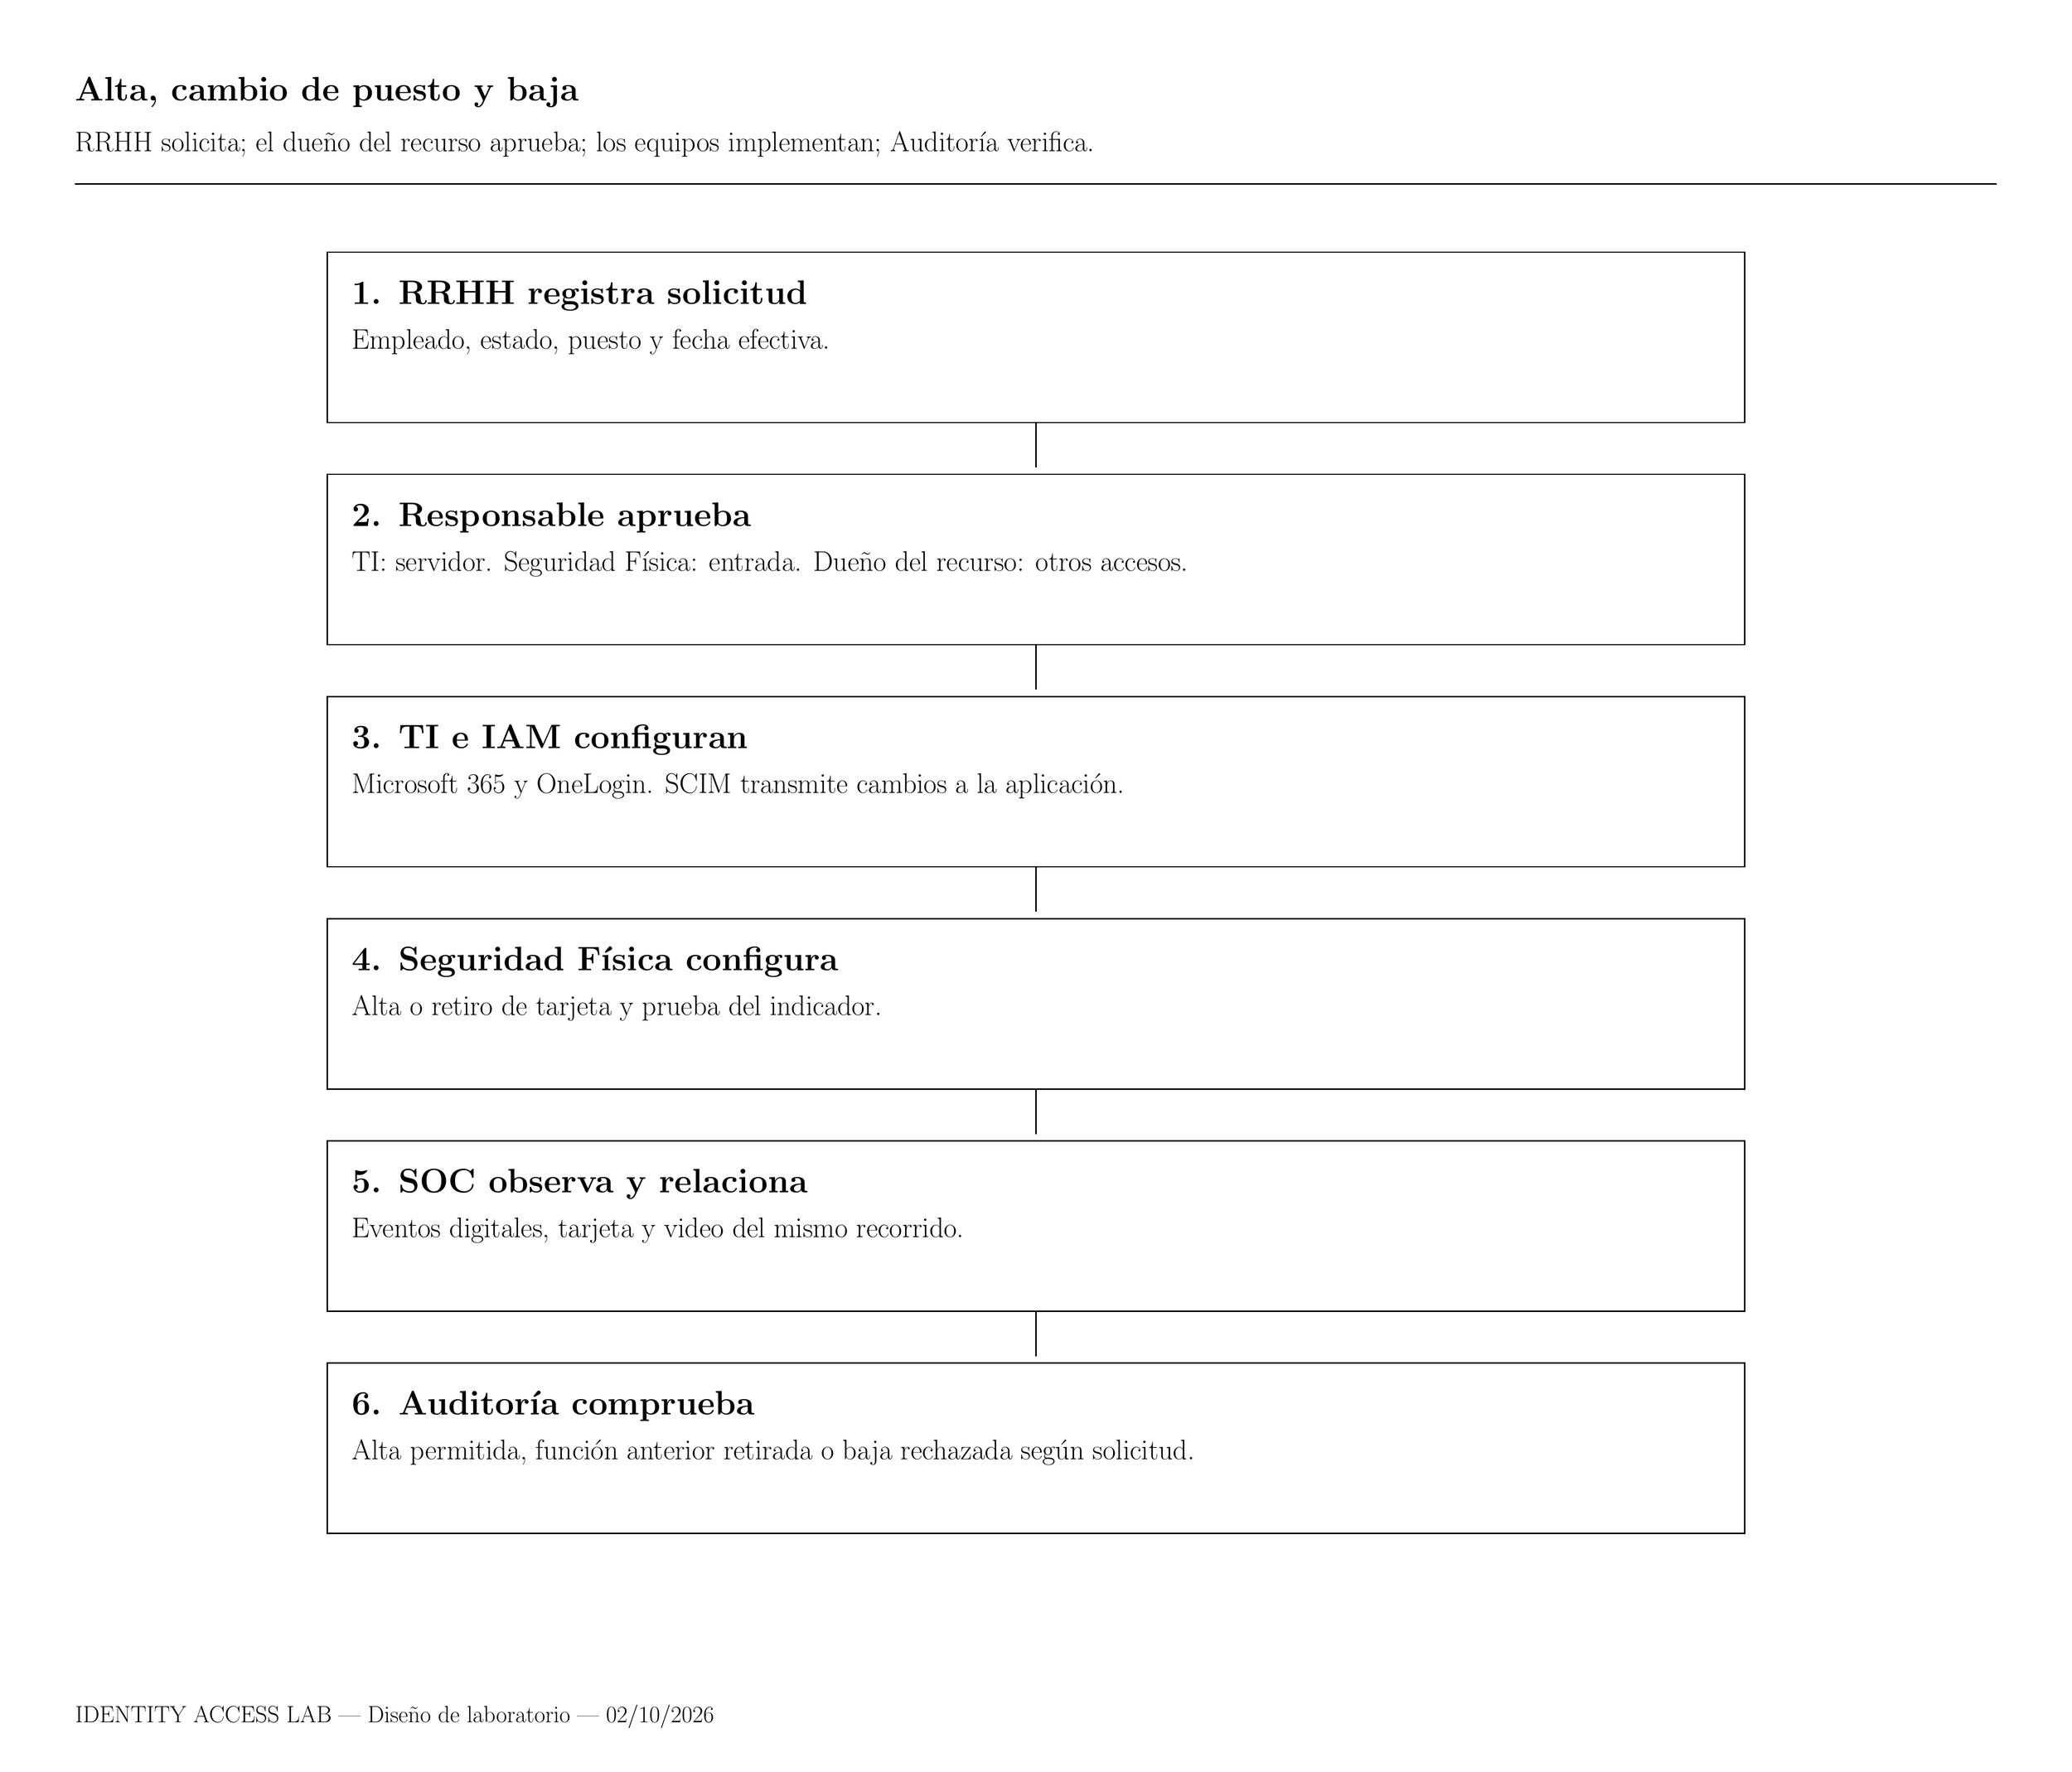
\begin{tikzpicture}[x=1pt,y=-1pt]
\path[use as bounding box] (0,0) rectangle (1500.0,1280.0);
\node[anchor=base west,inner sep=0pt,font=\fontsize{34.0}{40.8}\selectfont \bfseries ] at (45,64) {Alta, cambio de puesto y baja};
\node[anchor=base west,inner sep=0pt,font=\fontsize{21.0}{25.2}\selectfont ] at (45,101) {RRHH solicita; el dueño del recurso aprueba; los equipos implementan; Auditoría verifica.};
\draw[line width=1pt] (45,125) -- (1455,125);
\draw[line width=1pt] (230.0,175.0) rectangle (1270.0,300.0);
\node[anchor=base west,inner sep=0pt,font=\fontsize{24.0}{28.799999999999997}\selectfont \bfseries ] at (248,213) {1. RRHH registra solicitud};
\node[anchor=base west,inner sep=0pt,font=\fontsize{22.0}{26.4}\selectfont ] at (248,246) {Empleado, estado, puesto y fecha efectiva.};
\draw[line width=1pt] (750,300) -- (750,333);
\draw[line width=1pt] (230.0,338.0) rectangle (1270.0,463.0);
\node[anchor=base west,inner sep=0pt,font=\fontsize{24.0}{28.799999999999997}\selectfont \bfseries ] at (248,376) {2. Responsable aprueba};
\node[anchor=base west,inner sep=0pt,font=\fontsize{22.0}{26.4}\selectfont ] at (248,409) {TI: servidor. Seguridad Física: entrada. Dueño del recurso: otros accesos.};
\draw[line width=1pt] (750,463) -- (750,496);
\draw[line width=1pt] (230.0,501.0) rectangle (1270.0,626.0);
\node[anchor=base west,inner sep=0pt,font=\fontsize{24.0}{28.799999999999997}\selectfont \bfseries ] at (248,539) {3. TI e IAM configuran};
\node[anchor=base west,inner sep=0pt,font=\fontsize{22.0}{26.4}\selectfont ] at (248,572) {Microsoft 365 y OneLogin. SCIM transmite cambios a la aplicación.};
\draw[line width=1pt] (750,626) -- (750,659);
\draw[line width=1pt] (230.0,664.0) rectangle (1270.0,789.0);
\node[anchor=base west,inner sep=0pt,font=\fontsize{24.0}{28.799999999999997}\selectfont \bfseries ] at (248,702) {4. Seguridad Física configura};
\node[anchor=base west,inner sep=0pt,font=\fontsize{22.0}{26.4}\selectfont ] at (248,735) {Alta o retiro de tarjeta y prueba del indicador.};
\draw[line width=1pt] (750,789) -- (750,822);
\draw[line width=1pt] (230.0,827.0) rectangle (1270.0,952.0);
\node[anchor=base west,inner sep=0pt,font=\fontsize{24.0}{28.799999999999997}\selectfont \bfseries ] at (248,865) {5. SOC observa y relaciona};
\node[anchor=base west,inner sep=0pt,font=\fontsize{22.0}{26.4}\selectfont ] at (248,898) {Eventos digitales, tarjeta y video del mismo recorrido.};
\draw[line width=1pt] (750,952) -- (750,985);
\draw[line width=1pt] (230.0,990.0) rectangle (1270.0,1115.0);
\node[anchor=base west,inner sep=0pt,font=\fontsize{24.0}{28.799999999999997}\selectfont \bfseries ] at (248,1028) {6. Auditoría comprueba};
\node[anchor=base west,inner sep=0pt,font=\fontsize{22.0}{26.4}\selectfont ] at (248,1061) {Alta permitida, función anterior retirada o baja rechazada según solicitud.};
\node[anchor=base west,inner sep=0pt,font=\fontsize{18.0}{21.599999999999998}\selectfont ] at (45,1254) {IDENTITY ACCESS LAB | Diseño de laboratorio | 02/10/2026};
\end{tikzpicture}}
\clearpage
\noindent\resizebox{\textwidth}{!}{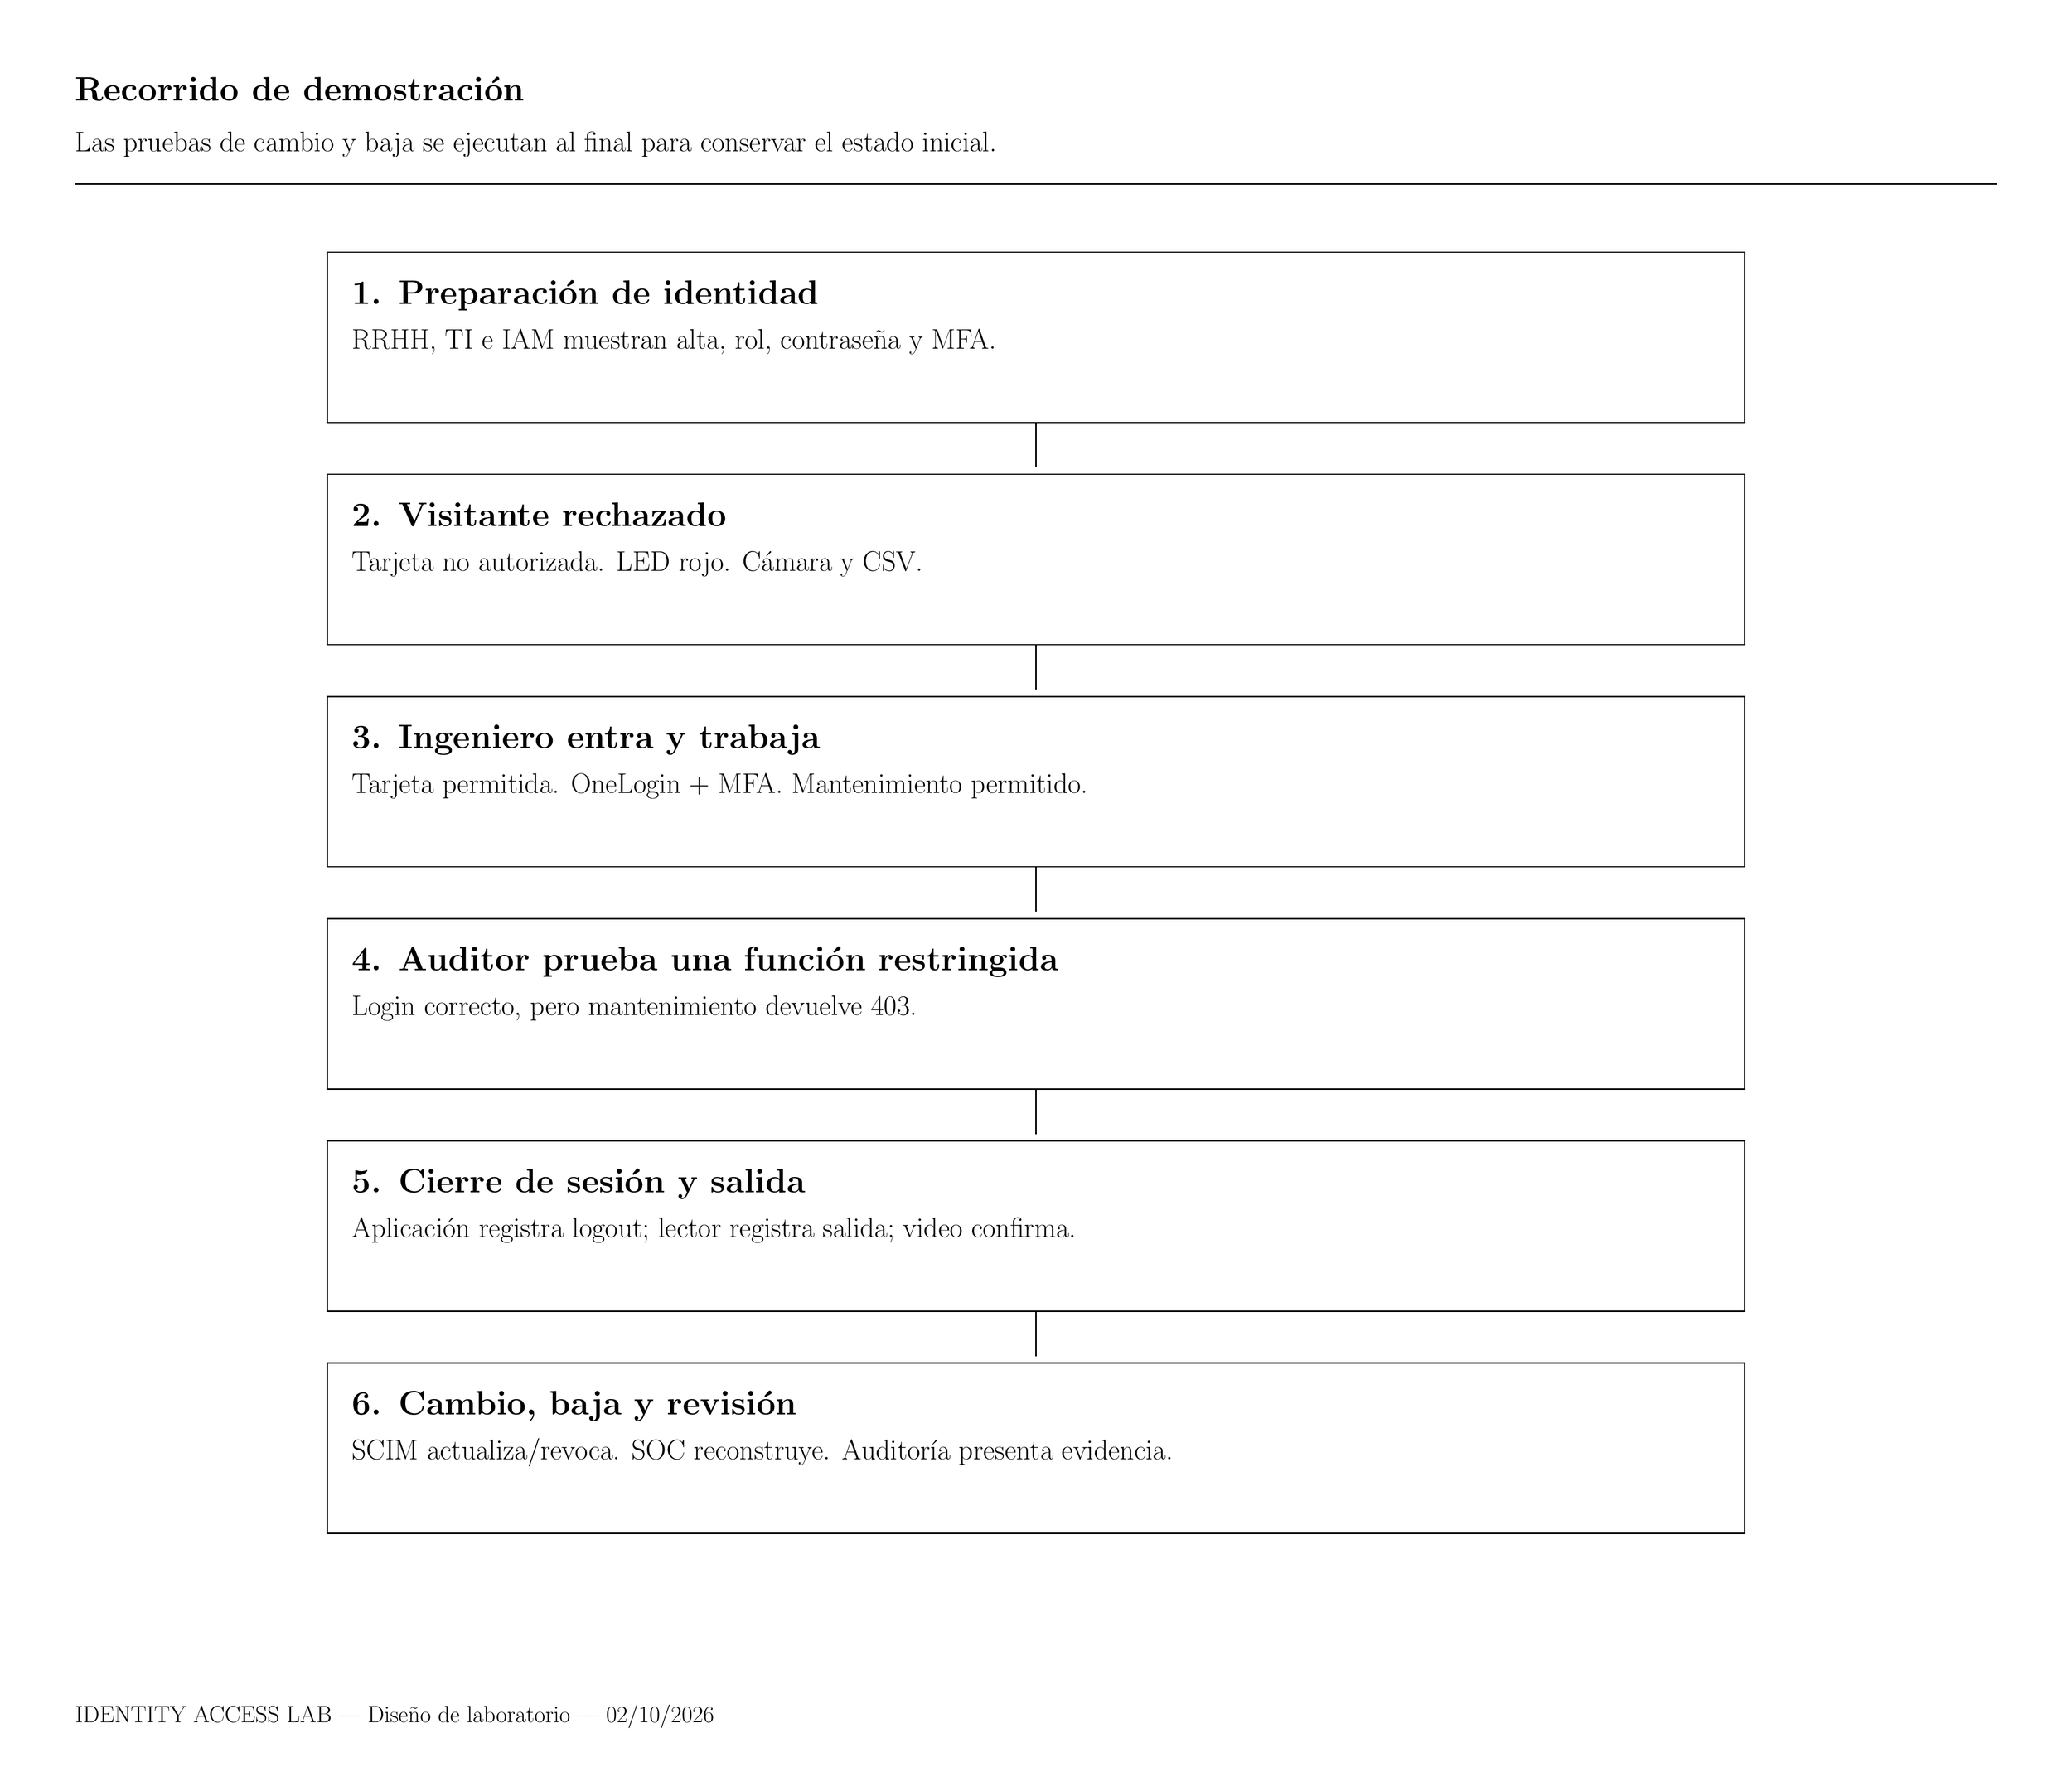
\begin{tikzpicture}[x=1pt,y=-1pt]
\path[use as bounding box] (0,0) rectangle (1500.0,1280.0);
\node[anchor=base west,inner sep=0pt,font=\fontsize{34.0}{40.8}\selectfont \bfseries ] at (45,64) {Recorrido de demostración};
\node[anchor=base west,inner sep=0pt,font=\fontsize{21.0}{25.2}\selectfont ] at (45,101) {Las pruebas de cambio y baja se ejecutan al final para conservar el estado inicial.};
\draw[line width=1pt] (45,125) -- (1455,125);
\draw[line width=1pt] (230.0,175.0) rectangle (1270.0,300.0);
\node[anchor=base west,inner sep=0pt,font=\fontsize{24.0}{28.799999999999997}\selectfont \bfseries ] at (248,213) {1. Preparación de identidad};
\node[anchor=base west,inner sep=0pt,font=\fontsize{22.0}{26.4}\selectfont ] at (248,246) {RRHH, TI e IAM muestran alta, rol, contraseña y MFA.};
\draw[line width=1pt] (750,300) -- (750,333);
\draw[line width=1pt] (230.0,338.0) rectangle (1270.0,463.0);
\node[anchor=base west,inner sep=0pt,font=\fontsize{24.0}{28.799999999999997}\selectfont \bfseries ] at (248,376) {2. Visitante rechazado};
\node[anchor=base west,inner sep=0pt,font=\fontsize{22.0}{26.4}\selectfont ] at (248,409) {Tarjeta no autorizada. LED rojo. Cámara y CSV.};
\draw[line width=1pt] (750,463) -- (750,496);
\draw[line width=1pt] (230.0,501.0) rectangle (1270.0,626.0);
\node[anchor=base west,inner sep=0pt,font=\fontsize{24.0}{28.799999999999997}\selectfont \bfseries ] at (248,539) {3. Ingeniero entra y trabaja};
\node[anchor=base west,inner sep=0pt,font=\fontsize{22.0}{26.4}\selectfont ] at (248,572) {Tarjeta permitida. OneLogin + MFA. Mantenimiento permitido.};
\draw[line width=1pt] (750,626) -- (750,659);
\draw[line width=1pt] (230.0,664.0) rectangle (1270.0,789.0);
\node[anchor=base west,inner sep=0pt,font=\fontsize{24.0}{28.799999999999997}\selectfont \bfseries ] at (248,702) {4. Auditor prueba una función restringida};
\node[anchor=base west,inner sep=0pt,font=\fontsize{22.0}{26.4}\selectfont ] at (248,735) {Login correcto, pero mantenimiento devuelve 403.};
\draw[line width=1pt] (750,789) -- (750,822);
\draw[line width=1pt] (230.0,827.0) rectangle (1270.0,952.0);
\node[anchor=base west,inner sep=0pt,font=\fontsize{24.0}{28.799999999999997}\selectfont \bfseries ] at (248,865) {5. Cierre de sesión y salida};
\node[anchor=base west,inner sep=0pt,font=\fontsize{22.0}{26.4}\selectfont ] at (248,898) {Aplicación registra logout; lector registra salida; video confirma.};
\draw[line width=1pt] (750,952) -- (750,985);
\draw[line width=1pt] (230.0,990.0) rectangle (1270.0,1115.0);
\node[anchor=base west,inner sep=0pt,font=\fontsize{24.0}{28.799999999999997}\selectfont \bfseries ] at (248,1028) {6. Cambio, baja y revisión};
\node[anchor=base west,inner sep=0pt,font=\fontsize{22.0}{26.4}\selectfont ] at (248,1061) {SCIM actualiza/revoca. SOC reconstruye. Auditoría presenta evidencia.};
\node[anchor=base west,inner sep=0pt,font=\fontsize{18.0}{21.599999999999998}\selectfont ] at (45,1254) {IDENTITY ACCESS LAB | Diseño de laboratorio | 02/10/2026};
\end{tikzpicture}}
\end{document}
